% REMEMBER: You must not plagiarise anything in your report. Be extremely careful.
\documentclass{l4proj}

    
%==============================================================================
% Put any additional packages here
% You can add any packages you want, as long as it does not alter
% the overall format (e.g. don't change the margins or the reference style).
%
\usepackage{pdfpages} % if you want to include a PDF for an ethics checklist, for example
%
%

\begin{document}

%==============================================================================
%% METADATA
\title{Model Checking for Strategy Generation in Football} % change this to your title
\author{Kevin E. Lynch}
\date{April 16, 2021}

\maketitle

%==============================================================================
%% ABSTRACT
\begin{abstract}
    \vskip 0.5em
    In his 2008 retrospective of the sport, \textit{Inverting the Pyramid} \cite{wils1}, Jonathan Wilson observed that football practitioners, particularly in the UK, have traditionally been \textit{"unwilling to grapple with the abstract."} In the past decade, however, abstractions of football have become invaluable. Teams increasingly rely on computer-aided analysis of match data to inform decisions, both on and off the pitch. This project investigates the feasibility of using model checking as a technique to gain insights from football data and identify potential strategies. 
    
    We show that event-level match data can be used in conjunction with modelling techniques and the PRISM probabilistic model checker to synthesise plausible football strategies, and attempt to lay a foundation for potential future work on this topic.
\end{abstract}

%==============================================================================
%% ACKNOWLEDGEMENTS
\chapter*{Acknowledgements}
% Enter any acknowledgements here. This is optional; you may leave this blank if you wish,
% or remove the entire chapter
%
I would like to thank both Professor Alice Miller and William Kavanagh for their guidance, support and patience throughout this project. 
%

%==============================================================================

% EDUCATION REUSE CONSENT FORM
% If you consent to your project being shown to future students for educational purposes
% then insert your name and the date below to  sign the education use form that appears in the front of the document. 
% You must explicitly give consent if you wish to do so.
% If you sign, your project may be included in the Hall of Fame if it scores particularly highly.
%
%
%
\def\consentname {Kevin E. Lynch} % your full name
\def\consentdate {16 April 2021} % the date you agree
%
\educationalconsent


%==============================================================================
\tableofcontents

%==============================================================================
%% Notes on formatting
%==============================================================================
% The first page, abstract and table of contents are numbered using Roman numerals and are not
% included in the page count. 
%
% From now on pages are numbered
% using Arabic numerals. Therefore, immediately after the first call to \chapter we need the call
% \pagenumbering{arabic} and this should be called once only in the document. 
%
%
% The first Chapter should then be on page 1. 

% PAGE LIMITS
% You are allowed 40 pages for a 40 credit project and 30 pages for a 
% 20 credit report. 
% This includes everything numbered in Arabic numerals (excluding front matter) up
% to but *excluding the appendices and bibliography*.
%
% FORMATTING
% You must not alter text size (it is currently 10pt) or alter margins or spacing.
% Do not alter the bibliography style. 
%
%==================================================================================================================================
%
% IMPORTANT
% The chapter headings and structure here are **suggestions**. You don't have to follow this model if
% it doesn't fit your project. Every project should have an introduction and conclusion,
% however.  If in doubt, your supervisor can give you specific guidance; their view takes precedence over
% the structure suggested here.
%
%==================================================================================================================================
\chapter{Introduction}

% reset page numbering. Don't remove this!
\pagenumbering{arabic} 

% You can use \todo{} to mark text that needs to be fixed. Anything inside will appear as highlighted 
% text in the final copy, and you will also get warnings when you compile (so you don't
% forget to take them out!)

\section{Motivation}

Association football is a complicated and unpredictable sport \cite{Brech20}. For the game's stakeholders, this can be of considerable concern, as the once humble game has become an incredibly high-stakes enterprise worldwide. UEFA, the Union of European Football Associations, reported revenue of €3.86 billion in the 2018/19 season \cite{Uefa19}. Barcelona F.C. generated €840.8 million in the same period, and, despite the impact of the COVID-19 pandemic, posted a turnover of €715.1 million for the extended 2019/20 season \cite{Delo21}.

With so much at stake, it is no surprise that football clubs are under pressure to invest heavily in commodities and activities intended to provide a competitive (and ultimately financial) advantage. Players, managers and coaching staff at the top levels are known to receive substantial remuneration \cite{SpI19} and the biggest clubs continue to spend money developing stadiums and other facilities \cite{Marca19}. In the past decade, teams at all levels have started to direct significant resources towards data science operations, in an effort to better inform decisions taken around training, transfer targets and on-the-pitch strategy. Meanwhile, third parties such as Opta, StatsBomb and Wyscout have emerged, turning football data collection and analysis into a lucrative business \cite{forb1}.

Data analysis has become a key activity at the biggest football clubs. The work of Ian Graham, Liverpool F.C.'s Director of Research \cite{lpool1}, is often cited in explaining the team's recent successes. Graham's team of analysts contributed heavily to decisions about recruitment, training and tactics which led to the club winning the UEFA Champions' League in 2019 \cite{nyt1} and the English Premier League in 2020 - their first European and domestic championships in 14 and 30 years, respectively.

Despite the proliferation of data-driven operations, this kind of football analysis is still emergent, and the community is actively seeking novel approaches which could generate even better insights. Professor Carlos Lago Peñas, in a 2020 blog post for Barcelona F.C.'s Innovation Hub, encapsulates the current state-of-the-art: 

\begin{quote}
\textit{"The tech revolution has modified our behaviour and now it is also revolutionizing sports. More and more tools are capable of collecting a great amount of data, which can help us make better decisions on the pitch. That is why it is interesting to capture all this data because it can help win matches. Although a great effort is done to improve the collection of data for real-time information, we still lack a good accurate interpretation of this information to help improve the coaches decisions"} \cite{barca1}.
\end{quote}

\textbf{Model checking} is an automatic technique for the formal analysis of models of a system \cite{pomc1}, initially developed to analyse hardware and software systems, but which has since been applied to systems as diverse as security protocols, industrial practices \cite{hmbc3}, and biological systems \cite{biomc1}. One application in particular is for strategy generation, or \textit{strategy synthesis}, whereby a model checker is used to determine an optimal course of action to satisfy some property or achieve some goal. Recent work has used model checking for strategy generation in video game mechanics \cite{kav1} and unmanned vehicle systems \cite{fac2}. We intend to investigate its application to the game of football.

\section{Specification}

The project specification (\textbf{Appendix \ref{appendix1}}) proposes an investigation into the viability of model checking as a tool for analysing football data. In particular, the project aims to demonstrate a use case for model checking in identifying "strategies with maximal scoring potential."

We have outlined a number of requirements and objectives for this project:

\begin{itemize}
    \item
    obtain and examine player data;
    \item
    build an \textit{expected goals} (xG) model from player data;
    \item
    develop PRISM models, simulating a sequence of choices (made by players) which have probabilistic outcomes (based on the player data);
    \item
    use the PRISM model checker, automatically determining which strategies are optimal (in terms of expected number of goals scored) for any given starting state. 
\end{itemize}

%Remember, you will be marked by your supervisor and one or more members of staff. You might also have your project read by a prize-awarding committee or possibly a future employer. Bear that in mind.

We were able to obtain an extensive public data set comprising over 3.2 million \textit{on-the-ball} events from top European leagues. While this data set is not as rich as those used by football clubs or football analytics companies such as StatsBomb \cite{sbomb1}, it allows for far greater fidelity of modelling than synthesised data would have. Further discussion of the data can be found in \textbf{Section \ref{data}}.

\section{Project Outline}

We begin with a brief overview, in simple terms, of the model checking methodology, and in particular probabilistic model checking. We then introduce the concepts of Markov chains and Markov decision processes, two closely related stochastic models that we will use to model the game of football, followed by a short examination of the PRISM model checker.

We conduct a high-level survey of related work in the field of football data analysis, as well as some published research on model checking applications, including strategy synthesis with PRISM.

We examine the data set that we will use for our research, and walk through the process of generating an \textit{expected goals} (xG) model. We also describe the process of building Markov models that are based upon the data.

Finally, we use PRISM to generate strategies based on our models, before evaluating our results and speculating about potential future work.

%==================================================================================================================================
\chapter{Background}

\section{Model Checking}

%\textbf{Definition of Model Checking -> its common uses}

Model checking is an automatic technique for the formal verification\footnote{Formal verification is "...the application of rigorous, mathematics-based techniques to establish the correctness of computerised systems" \cite{dpox1}.} of models which are abstractions of large and complex systems, where manual analysis would be impractical or unreliable. Traditionally it has been used in engineering fields such as aerospace, medical technology, computer architecture and telecommunications \cite{pomc1, hbmc1}. Model checkers exhaustively explore the state space (the set of possible states that a modelled system may find itself in), in order to verify specified properties such as correctness, safety, or the absence of deadlock states \cite{hbmc1}.

\begin{figure}[h]
    \centering
    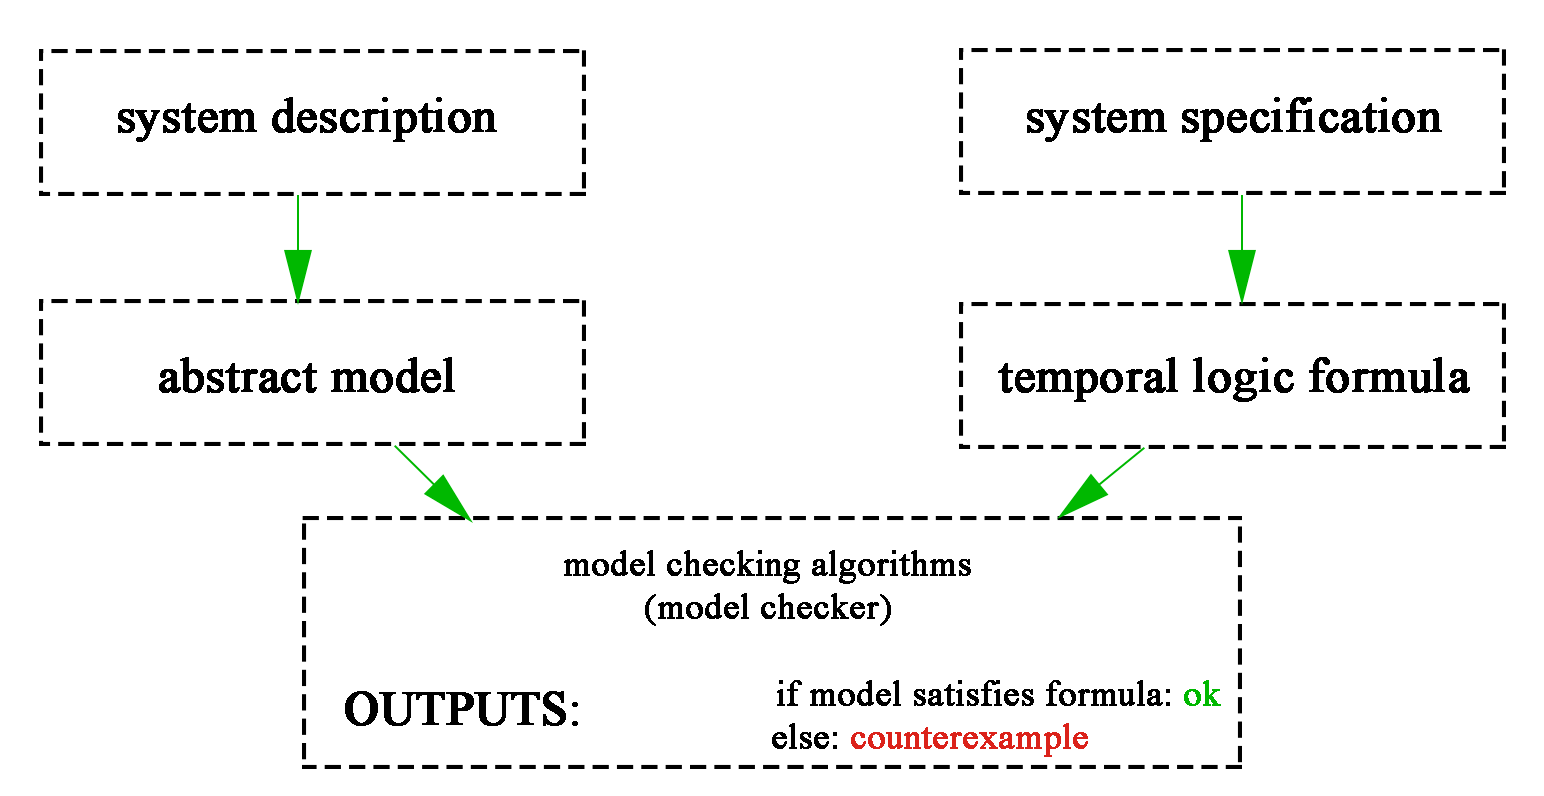
\includegraphics[scale=0.25]{images/mcheckdiag.png}   
    \caption{Diagram of the basic model checking methodology, adapted from Clarke, Henzinger and Veith's diagram in \cite{hbmc1}.}
    \label{fig:mcheckdiag} 
\end{figure}

There are three fundamental steps in model checking, which Clarke, Henzinger and Veith label \textit{modelling}, \textit{specification} and \textit{algorithms} \cite{hbmc1}. \textbf{Fig. \ref{fig:mcheckdiag}} shows an overview of how these stages interact, with modelling (on the left) and specification (on the right) creating inputs to algorithms (i.e. model checking software) at the bottom. 

\textit{Modelling} is accomplished by producing an abstract model (for example, a finite state-transition graph) which provides a high-level representation of the reachable states of a system (as nodes) and the transitions between them (as edges).

The \textit{specification} stage involves translating a set of properties that we wish to check (properties which, if satisfied, would prove the model's \textit{correctness}, \textit{liveness} etc.) into a formula expressed in a \textit{temporal logic} that the model checker can understand.

Finally, \textit{algorithms} refers to model checking algorithms which are usually implemented in a model checker. This software takes the model and temporal logic formula as inputs, and produces an output which indicates which properties are satisfied (or otherwise) by the model.

\subsection{Probabilistic Model Checking}

Probabilistic model checking is a branch of model checking concerned with verifying properties of inherently probabilistic systems. Whereas the classical model checking paradigm aims to prove deterministic properties (such as \textit{liveness}), probabilistic model checking allows us to reason quantitatively about randomized, unpredictable, or non-deterministic behaviours. Systems which exhibit such behaviours can be represented by stochastic models such as Markov chains and their variants \cite{hmbc2, pomc1, dpox1}. As such, Markov chains are well suited for the modelling and subsequent analysis of stochastic, real-world systems across  many domains \cite{hmbc2}, including biology, epidemiology, and even sports. 

This investigation focuses on probabilistic model checking, representing sequences of actions in football as Markov chains and Markov decision processes. The resultant systems are then verified using the PRISM model checker, with properties specified in PRISM's \textit{property specification language} - a modified temporal logic\footnote{A temporal logic is "[a] formal language for specifying and reasoning about how the behaviour of a system changes over time," which can be used to represent properties that we wish to test in a model checker \cite{dpox1}.} for use with PRISM.

%\textbf{Types of Model -> Markov Chains, Markov Decision processes, LTL}

\subsection{Discrete-time Markov Chains}

Markov chains are probabilistic transition systems. Baier and Katoen \cite{pomc1} explain that, given a set of states in a Markov chain, \textit{"the successor state of state \textit{s}... is chosen according to a probability distribution."} Furthermore, this probability distribution does not depend on any transitions that have occurred previously; they are uniquely associated with the current state. This is called \textit{memorylessness}, or the \textit{Markov property} \cite{pton1, dpox1}.

\begin{figure}[h]
    \centering
    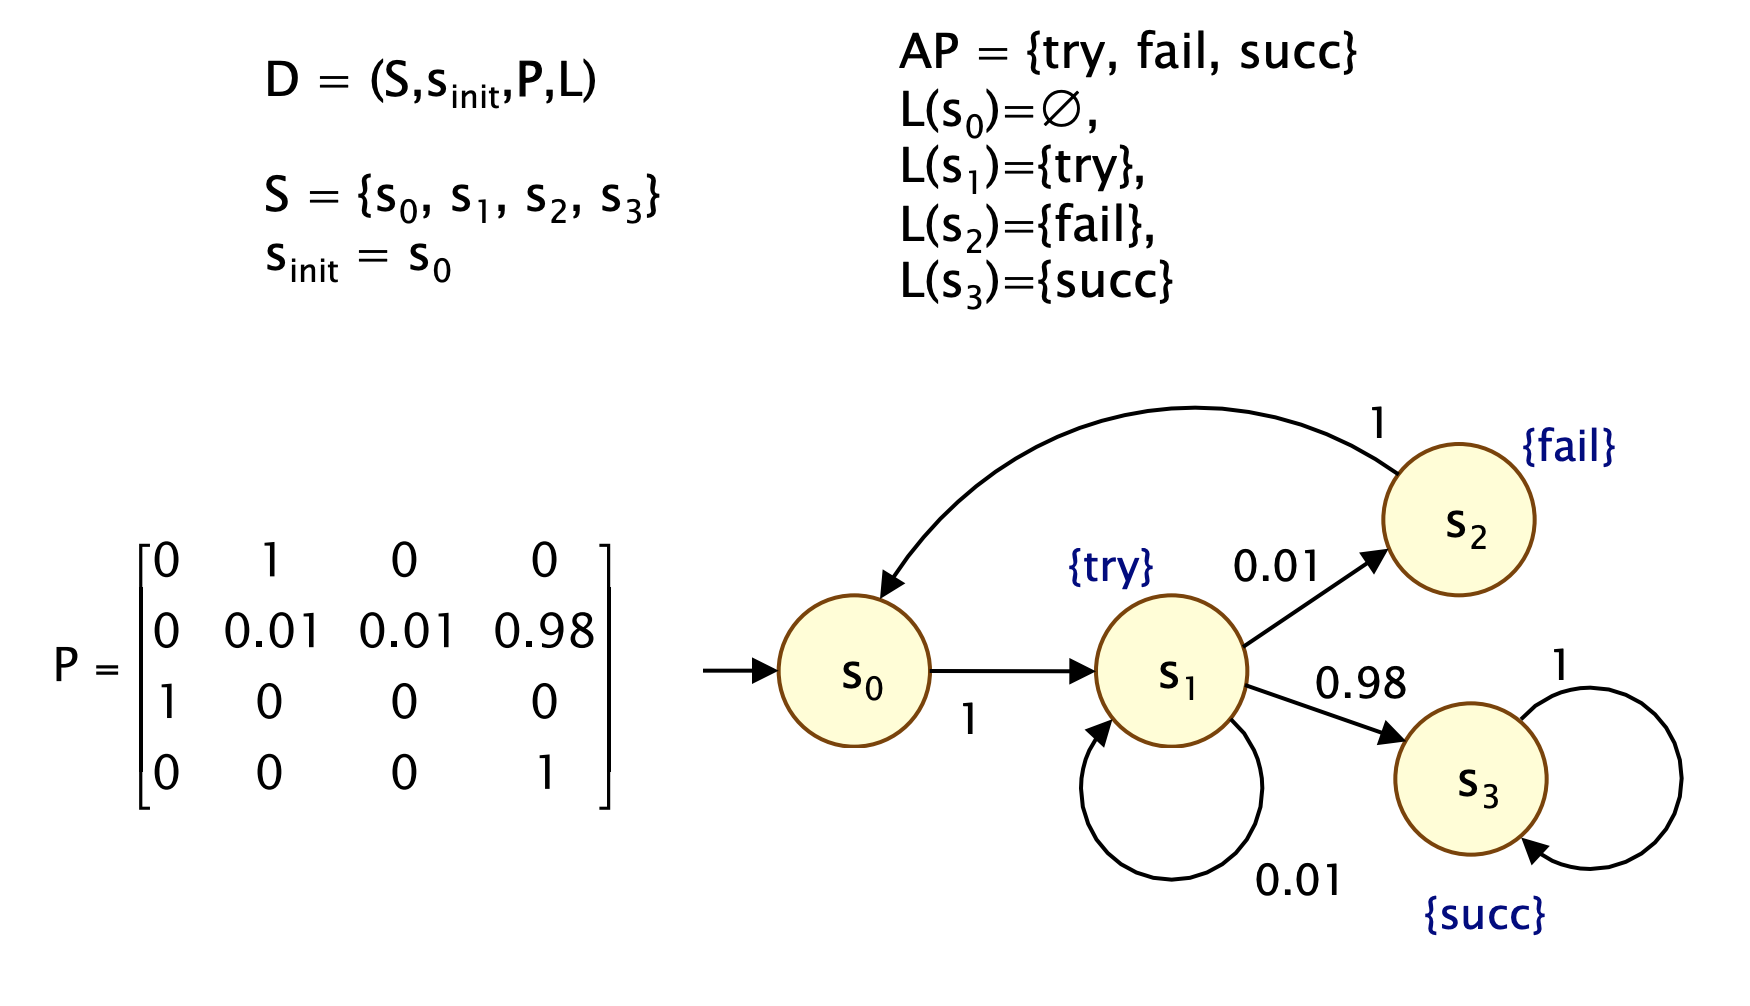
\includegraphics[scale=0.4]{images/dtmcdiag1.png}   
    \caption{An example of a DTMC, modelling a simple communications protocol \cite{dpox1}.}
    \label{fig:dtmcdiag} 
\end{figure}

A discrete-time Markov chain (DTMC), $D$, can be formalised as a tuple, $D = (S, s_{init}, P, L)$, where:

\begin{itemize}
    \item $S$ is the set of all reachable states (the state space);
    \item $s_{init}$ is the initial or starting state ($s_{init} \in S$);
    \item $P: S \times S$ is the \textit{transition probability matrix};
    \item $L : S \to 2^{AP}$ is a state-labelling function, where $AP$ is a set of state labels.
\end{itemize}

The \textit{transition probability matrix}, $P$, catalogues the probabilities of moving to any other state from the current state. $P$ is a \textit{stochastic matrix}, which by definition satisfies the conditions: \[P(s, s') \in [0,1] \textnormal{ \textit{(for all }} s, s' \in S \textnormal{\textit{)}}\] \[\sum_{s' \in S} P(s, s') \leq 1 \textnormal{ \textit{(for all }} s \in S \textnormal{\textit{)}}\]

We must also consider \textit{absorbing states}, which are states for which $P(s,s) = 1$; in other words, once this state has been reached, the system stays in it.

The DTMC shown in \textbf{Fig. \ref{fig:dtmcdiag}} represents a simple communications protocol. Of note are the outgoing edges of $s_{1}$, indicating the probabilities of each transition, and the absorbing state $s_{3}$.

Finally, the qualifier "discrete-time" is indicative of the fact that transitions occur in discrete time-steps (e.g. a CPU clock tick) \cite{dpox1}.

\subsection{Markov Decision Processes}

A Markov decision process (MDP) is an extension of a DTMC which allows for \textit{non-deterministic choice} \cite{pomc1}. As with DTMCs, transitions occur at discrete time-steps. Unlike DTMCs, there is a \textit{decision} taken at each step - a non-deterministic choice from a set of actions, each of which has its own probability distribution over possible successor states \cite{dpox1}.

\begin{figure}[h]
    \centering
    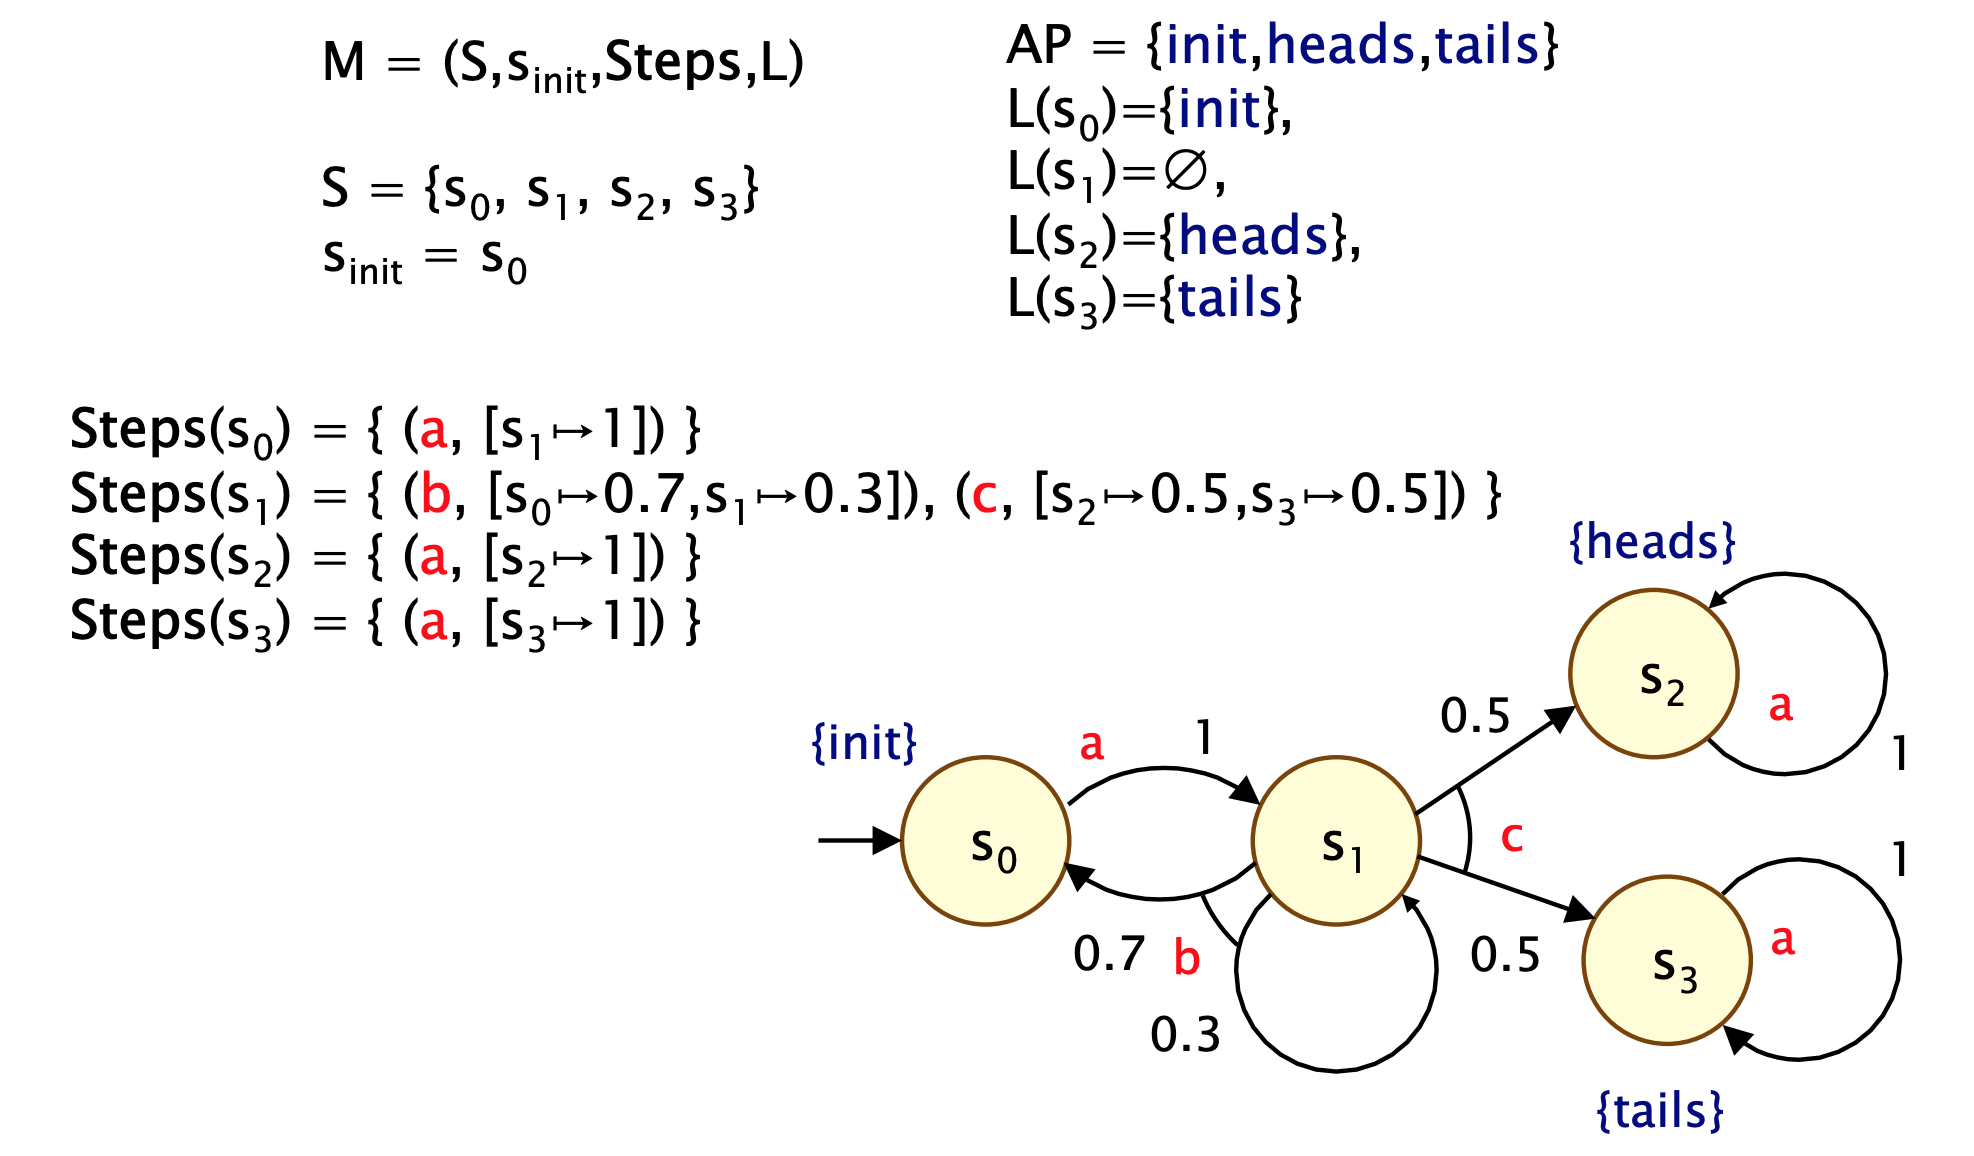
\includegraphics[scale=0.4]{images/mdpdiag1.png}   
    \caption{An example of an MDP, modelling a coin toss \cite{dpox1}.}
    \label{fig:mdpdiag} 
\end{figure}

An MDP, $M$, can be formally specified as a tuple, $M = (S, s_{init}, Steps, L)$, where:

\begin{itemize}
    \item $S$ is the set of all reachable states (the state space);
    \item $s_{init}$ is the initial or starting state ($s_{init} \in S$);
    \item $Steps : S \to 2^{Act \times Dist(S)}$ is the \textit{transition probability function}, where $Act$ is a set of possible actions, and $Dist(S)$ is the set of discrete probability distributions over $S$;
    \item $L : S \to 2^{AP}$ is a state-labelling function, where $AP$ is a set of state labels.
\end{itemize}

The concept of an absorbing state carries over from DTMCs, as does the constraint that probabilities sum to 1, but in the case of MDPs this is applied to the probability distribution associated with a given action. 

The diagram in \textbf{Fig. \ref{fig:mdpdiag}} illustrates the actions available to the system at $s_{1}$. When executing this system, a non-deterministic choice is made at $s_{1}$ between actions $b$ and $c$, each of which has its own set of transition probabilities. This is of particular use as it allows us to model decisions made by some autonomous agent (e.g. a human user) and their outcomes.

\subsection{The PRISM Model Checker}

PRISM \cite{KNP11} is "a \textit{probabilistic model checker}" used to model and analyse \textit{"systems that exhibit random or probabilistic behaviour,"} \cite{pweb1}. The ability to check such stochastic systems distinguishes PRISM from many other model checking tools, such as SPIN \cite{spin}, and allows us to quantify properties like performance or reliability. As with other model checkers, we describe a model in a high-level modelling language, from which a meticulous mathematical model is derived by the software. We then provide formal property specifications in temporal logic, and the model checker analyses our model with respect to the given properties.

We model systems for PRISM using the PRISM language, \textit{"a simple, state-based language"} \cite{prsmlang} based on the work of Alur and Henzinger \cite{AH99}. The PRISM language is primarily composed of \textit{modules} and \textit{variables}. When specifying a model, we define modules which can interact with one another. Each module has an associated set of variables. The set of  realizations of all of the variables for a model is its state space.

Module behaviours are specified by \textit{commands}, the syntax of which is shown in \textbf{Fig. \ref{fig:prsmcmd}}.

\begin{figure}[h]
    \centering
    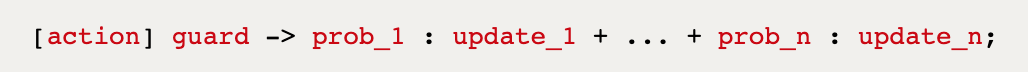
\includegraphics[scale=0.6]{images/commandexample.png}   
    \caption{Syntax of a PRISM command, taken from the PRISM manual \cite{prsmlang}.}
    \label{fig:prsmcmd} 
\end{figure}

Changes in system state are described by the \texttt{update} statements. When the expression in \texttt{guard} evaluates to true, \texttt{update\_n} can occur with probability \texttt{prob\_n}. The optional \texttt{action} string can be used to label transitions, or to enable PRISM's synchronisation features.

The PRISM language can express all of the types of model that PRISM supports \cite{prsmlang}. In the course of this investigation, we use it to describe DTMCs and MDPs. 

Below is a simple example of a DTMC defined in the PRISM language (\textbf{Listing 2.1}). In this example, we have defined a model of the simple communications protocol examined previously (\textbf{Fig. \ref{fig:dtmcdiag}}). The module \texttt{comms} has a variable \texttt{s} which can represent each of our states, $s_0$ to $s_3$. Each of the commands has been labelled (with the exception of the command associated with the initial state), consistent with the earlier diagram.

The simplicity of the PRISM language allows us to easily determine all possible behaviours from the listing. For example, in the initial state $s_0$, we always advance to $s_1$. The command fired when \texttt{s = 1} is labelled \texttt{try}, and the model will either:

\begin{itemize}
    \item remain in $s_1$ (continue trying) with probability $P = 0.01$;
    \item advance to $s_2$ (fail to send a message) with probability $P = 0.01$;
    \item advance to $s_3$ (successfully send a message) with probability $P = 0.98$.
\end{itemize}

\clearpage
\begin{lstlisting}[language=Haskell, numbers=left, caption=A DTMC representation in the PRISM modelling language. This excerpt describes the simple communications protocol depicted in \textbf{Fig. \ref{fig:dtmcdiag}}.] 
dtmc 

module comms

	s : [0..3] init 0;
	[] s = 0 -> (s' = 1);
	[try] s = 1 -> 0.01 : (s' = 1) + 0.01 : (s' = 2) + 0.98 : (s' = 3);
	[fail] s = 2 -> (s' = 0);
    [succ] s = 3 -> (s' = 3);

endmodule
\end{lstlisting}

We can use PRISM's \textit{property specification language} to define properties of the model and formulate queries that we would like to evaluate. This language is based on temporal logic, and incorporates existing probabilistic temporal logics, including Probabilistic Computational Tree Logic (PCTL) and Linear Temporal Logic (LTL). Property queries in PRISM take the form:

\begin{center}
    \texttt{operator bound [ path\_property ]}
\end{center}

The property specification language offers several \texttt{operator}s, including \textbf{P} (probability), \textbf{S} (\textit{long-run} or \textit{steady-state} probability) and \textbf{R} (for specifying reward or cost-based queries). The \texttt{bound} is some numerical value, and the \texttt{path\_property} is some condition we are checking for. As an example, we can define a query:

\begin{center}
    \texttt{\textbf{P} >= 1 [ \textbf{F} s=3 ]}
    
    (where \textbf{F} means \textit{eventually})
\end{center}

This can be read as, \textit{"The probability that s will eventually be equal to 3 is greater than or equal to 1."} In the context of our simple system, we are asking the model checker, \textit{"will a message eventually be sent?"} By supplying PRISM with the model and a property, we can \textit{evaluate} the query. PRISM's output confirms that this property is true for our model.

\begin{center}
    \texttt{Result: true (property satisfied in the initial state)}
\end{center}

If we wanted to check the message failure probability against some threshold, we could specify a property such as:

\begin{center}
    \texttt{\textbf{P} >= 0.5 [ \textbf{F} s=2 ]}
\end{center}

Again, we can verify this property with respect to our model:

\begin{center}
    \texttt{Result: false (property not satisfied in the initial state)}
\end{center}

PRISM tells us that the probability of reaching $s_2$, the \texttt{fail} state, \textbf{is not} greater than or equal to \( \frac{1}{2} \). If we want to calculate what the probability is, we can replace our \texttt{bound} with \texttt{?}:

\begin{center}
    \texttt{\textbf{P} = ? [ \textbf{F} s=2 ]}
\end{center}

Rather than provide a boolean response, PRISM can \textit{quantitatively} evaluate this property, and provide a numerical result:

\begin{center}
    \texttt{Result: 0.010101010101010102 (value in the initial state)}
\end{center}

The probability that a message will fail is approximately 0.01; whereas this is straightforward to read from our simple model, the benefits of this sort of analysis when working with more complex systems should be clear.

\begin{lstlisting}[language=Haskell, numbers=left, caption=An MDP representation in the PRISM modelling language. This excerpt describes the simple coin toss model depicted in \textbf{Fig. \ref{fig:mdpdiag}}.] 
mdp

module coin

	s : [0..3] init 0;
	
	[a] s = 0 -> (s' = 1);
	[b] s = 1 -> 0.3 : (s' = 1) + 0.7 : (s' = 0);
	[c] s = 1 -> 0.5 : (s' = 2) + 0.5 : (s' = 3);
	[a] s = 2 -> (s' = 2);
	[a] s = 3 -> (s' = 3);

endmodule

label "heads" = (s=2);
label "tails" = (s=3);
\end{lstlisting}

\textbf{Listing 2.2} contains an example of an MDP, describing the model from \textbf{Fig. \ref{fig:mdpdiag}} of a coin toss. In this example, there are two commands with the same guard, \texttt{s = 1}. This represents the non-deterministic choice that is available in that state. 

By observing a step-by-step simulation from PRISM's GUI, we can confirm the possibility of either course of action - \texttt{a} or \texttt{b}.

\begin{figure}[h]
    \centering
    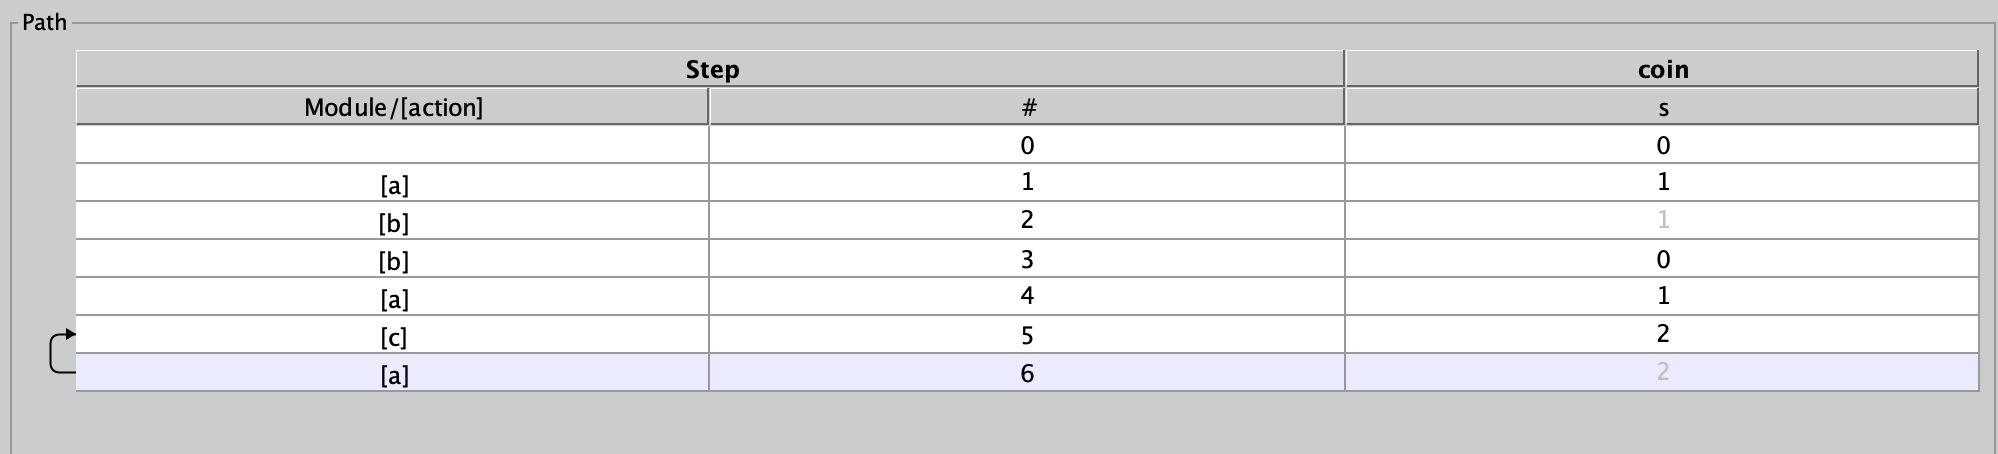
\includegraphics[scale=0.39]{images/simpath.png}   
    \caption{Simulation output of the PRISM model in \textbf{Listing 2.2}. The state $s$ at each step is in the rightmost column, and the action taken at each step is in the leftmost column. This trace shows that different choices have been made while in $s_1$, and that the same action can have different outcomes.}
    \label{fig:simpath} 
\end{figure}

As with the DTMC example, we can specify properties to check against the model. \textbf{Listing 2.2} includes examples of PRISM's \textit{label} feature which allows us to group together a set of states under a shorthand name (although in this instance, we only have one state variable). As such we can specify a property in the following manner:

\begin{center}
    \texttt{\textbf{Pmax} = ? [ \textbf{F} "heads" ]}
\end{center}

When checking a model with non-deterministic behaviour, probabilities are checked over "all possible resolutions of non-determinism," \cite{prsmlang} - in other words, \textit{over all possible paths of execution}. This property can be read as "What is the maximum probability, across all paths, that we will reach $s_2$ (heads)?" Once again, PRISM provides a numerical result:

\begin{center}
    \texttt{Result: 0.5 (value in the initial state)}    
\end{center}

Finally, we examine PRISM's reward structures. Rewards in PRISM can be assigned to states (or sets of states) or actions, in order to ascribe some benefit or cost to system behaviours. This allows us to record the number of times a particular system state has been visited, and also to define properties based upon these reward values.

\begin{lstlisting}[language=Haskell, numbers=left, caption=A simple reward structure which could be appended to our MDP example.] 
rewards "tosses"
	s=1 : 1;
endrewards
\end{lstlisting}

\textbf{Listing 2.3} shows a reward structure appended to the PRISM model in \textbf{Listing 2.2}, which adds a value of 1 to the \texttt{tosses} reward each time $s_1$ is visited. With this defined, we can specify a reward-based property, using the \textbf{R} operator. If we wanted to determine the minimum number of times $s_1$ is visited on the path to an end result, we can check the property:

\begin{center}
    \texttt{\textbf{R}\{"tosses"\}min=? [ ( \textbf{F} "heads" | \textbf{F} "tails" ]}    
\end{center}

Once more, PRISM returns a numerical result:

\begin{center}
    \texttt{Result: 1.0 (value in the initial state)}    
\end{center}

It is evident, looking at the graph in \textbf{Fig. \ref{fig:mdpdiag}}, that we have to pass through $s_1$ at least once to reach an absorbing state. However, as models become more complex, PRISM's features become increasingly useful.

\section{Football - The Beautiful Game}

At its simplest, football is a team sport, played by two opposing teams of eleven players each, in which the objective is to move a ball into the opposing team's goal, situated at the far end of the rectangular, symmetrical field of play \cite{ifab1}.

\begin{figure}[h]
    \centering
    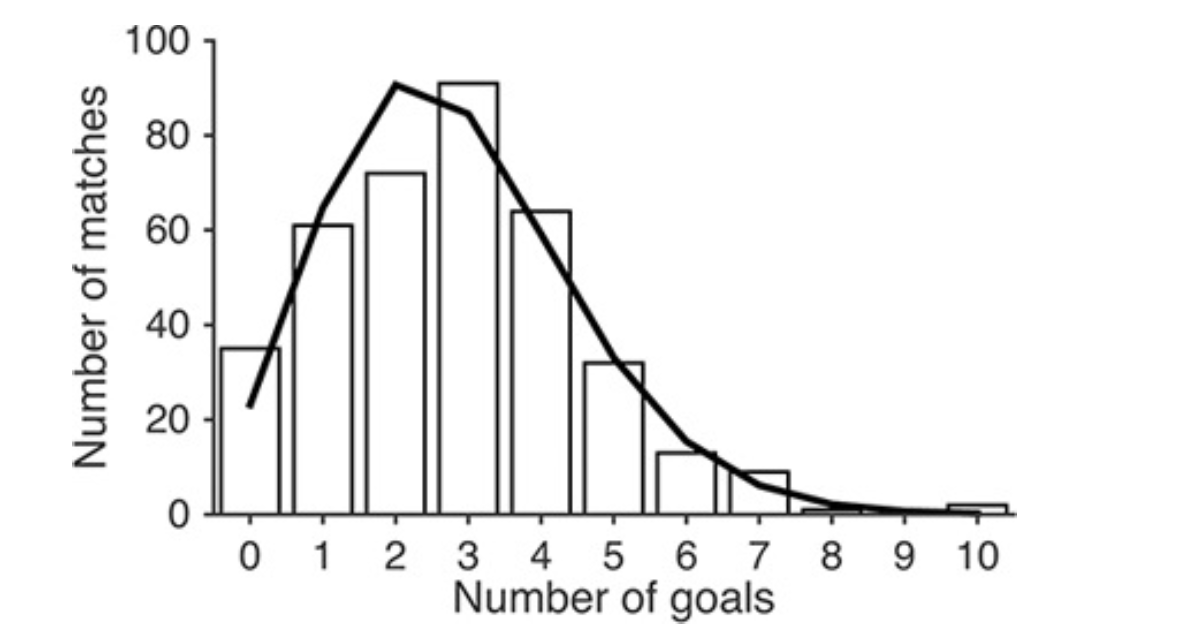
\includegraphics[scale=0.4]{images/pois1.png}   
    \caption{A historgram of the number of goals scored per game in the English Premier League 2012-13. The solid line shows the output of a simulation based only on probabilities; a Poisson distribution. Figure reproduced from Soccermatics, 2016 \cite{sump1}.}
    \label{fig:pois} 
\end{figure}

In his 2016 book \textit{Soccermatics} \cite{sump1}, mathematician David Sumpter observes that many aspects of football are random. As an example, he examines the English Premier League's 2012-13 season. Over the 380 fixtures that were played, there was an average of 2.79 goals scored per game. Sumpter therefore models a game of football in this season as:

\begin{quote}
    \textit{"...90 single-minute slots, in each of which a goal is equally likely... the probability that there is a goal in any one of these slots is $2.79/90 = 0.031$"} \cite{sump1}. 
\end{quote} 

Simulating this model many times and recording the number of goals scored per game results in a Poisson distribution\footnote{A concise explanation of Poisson distributions and processes can be found in Will Koehrsen's article on \textit{towardsdatascience.com} \cite{koe1}}. Sumpter shows this (in \textbf{Fig. \ref{fig:pois}}) as a solid line plotted over a histogram of the actual number of goals scored per game in that season. The results from the simulation very closely capture the shape of the distribution of goals scored. This randomness is indicative of the unpredictability of football. The implication is that football can be modelled as a system whose behaviour is \textit{probabilistic}.

The prevalence of data-driven strategy in other sports is in stark contrast to its slow uptake in football. Whereas major football clubs only started to make serious use of analytics during the past 5-10 years \cite{fcb2, guar1}, the practice has been transformative in other games since the early 2000s. The most famous example of a data-driven sporting success is that of the Oakland Athletics, an American baseball team, in 2002. Manager Billy Beane eschewed conventional baseball wisdom and instead leveraged the data, defying the odds and leading his team of underdogs on an unprecedented 20-game winning run (chronicled in the 2003 book \textit{Moneyball} \cite{mbal1}). Basketball, similarly, can trace its reliance on quantitative analysis to the late 1990s, with coach and statistician Dean Oliver publishing his blueprint for the approach, \textit{Basketball on Paper}, in 2003 \cite{bbop1}. 

Bornn \textit{et al.} put forward their own reasons for football's slow adoption of data science:

\begin{quote}
    \textit{"While the delay in the soccer community's acceptance of quantitative metrics might be attributed to its traditional and well‐entrenched culture... the data are also to blame. The problem for soccer is this: data across all major team sports have focused on what is happening to the ball throughout the game. In baseball, for instance, tracking ball events alone captures nearly every impactful moment in the game"} \cite{bornn1}.
\end{quote}

Basketball may be closer to football in terms of objective and possession mechanics, but with teams of only five `outfield' players and an area less than 10\% the size of a football pitch, passages of play are much easier to model. The relative challenge of modelling and analysing football is one of \textit{complexity}. 

\section{Related Work - The Rise of Data in Football}

One of the earliest examples of \textit{"football analytics"} is the work of Charles Reep, who worked as a tactical advisor at clubs including Wolverhampton Wanderers and Sheffield Wednesday in the 1950s. His influential 1968 article \textit{Skill and Chance in Association Football} \cite{reep1} provided the foundations for the \textit{long-ball} approach, which dominated English football in late 20th century \cite{wils1}.

Despite this, the football establishment dismissed the notion that maths and science could improve footballing tactics, and until recently there was very little activity of note. \textit{Moneyball}'s adaptation into an Oscar-nominated film in 2008 brought sports analytics and data science to the mainstream, and in the years since there have been significant works published that have had real consequences for football. We suggest that this is due to a number of factors - the increasing ubiquity of the internet, availability of data and tools for analysis, and interest in funding for serious research, from private analytics companies and football clubs alike. Myriad approaches have been advanced and are in use, and a number of frameworks for analysis have a basis in Markov models.

\subsection{Rudd's Markov Chains (2011)}

In 2011, analytics start-up StatDNA published match data that they had collected over the previous season of the English Premier League and invited the public to submit their own analyses, with the best contributors being invited to present their findings at the New England Symposium on Statistics in Sports at Harvard \cite{sump1}. The winner was Sarah Rudd, a software engineer, who gave the presentation \textit{A Framework for Tactical Analysis and Individual Offensive Production Assessment in Soccer Using Markov Chains} in September that year \cite{rudd1}. Although Rudd cited Keith Goldner's similar work \cite{gold1} on American football as an inspiration, this was broadly regarded as new territory for association football. 

Rudd's work divided a period of possession during a football match into 39 states based on the ball's location on the pitch, the players' positions and "dead-ball" or "set piece" situations\footnote{Scenarios where the ball is not in "open play", e.g. free kicks, throw-ins, corners.}. This included two absorbing states for a goal scored or possession lost. The motivation was to observe how the probability of a goal being scored changed as the possession moved from state to state, and assign credit to the players who enacted the state transitions accordingly.

\begin{figure}[htb] 
    \centering
    \begin{subfigure}[a]{0.75\textwidth}
        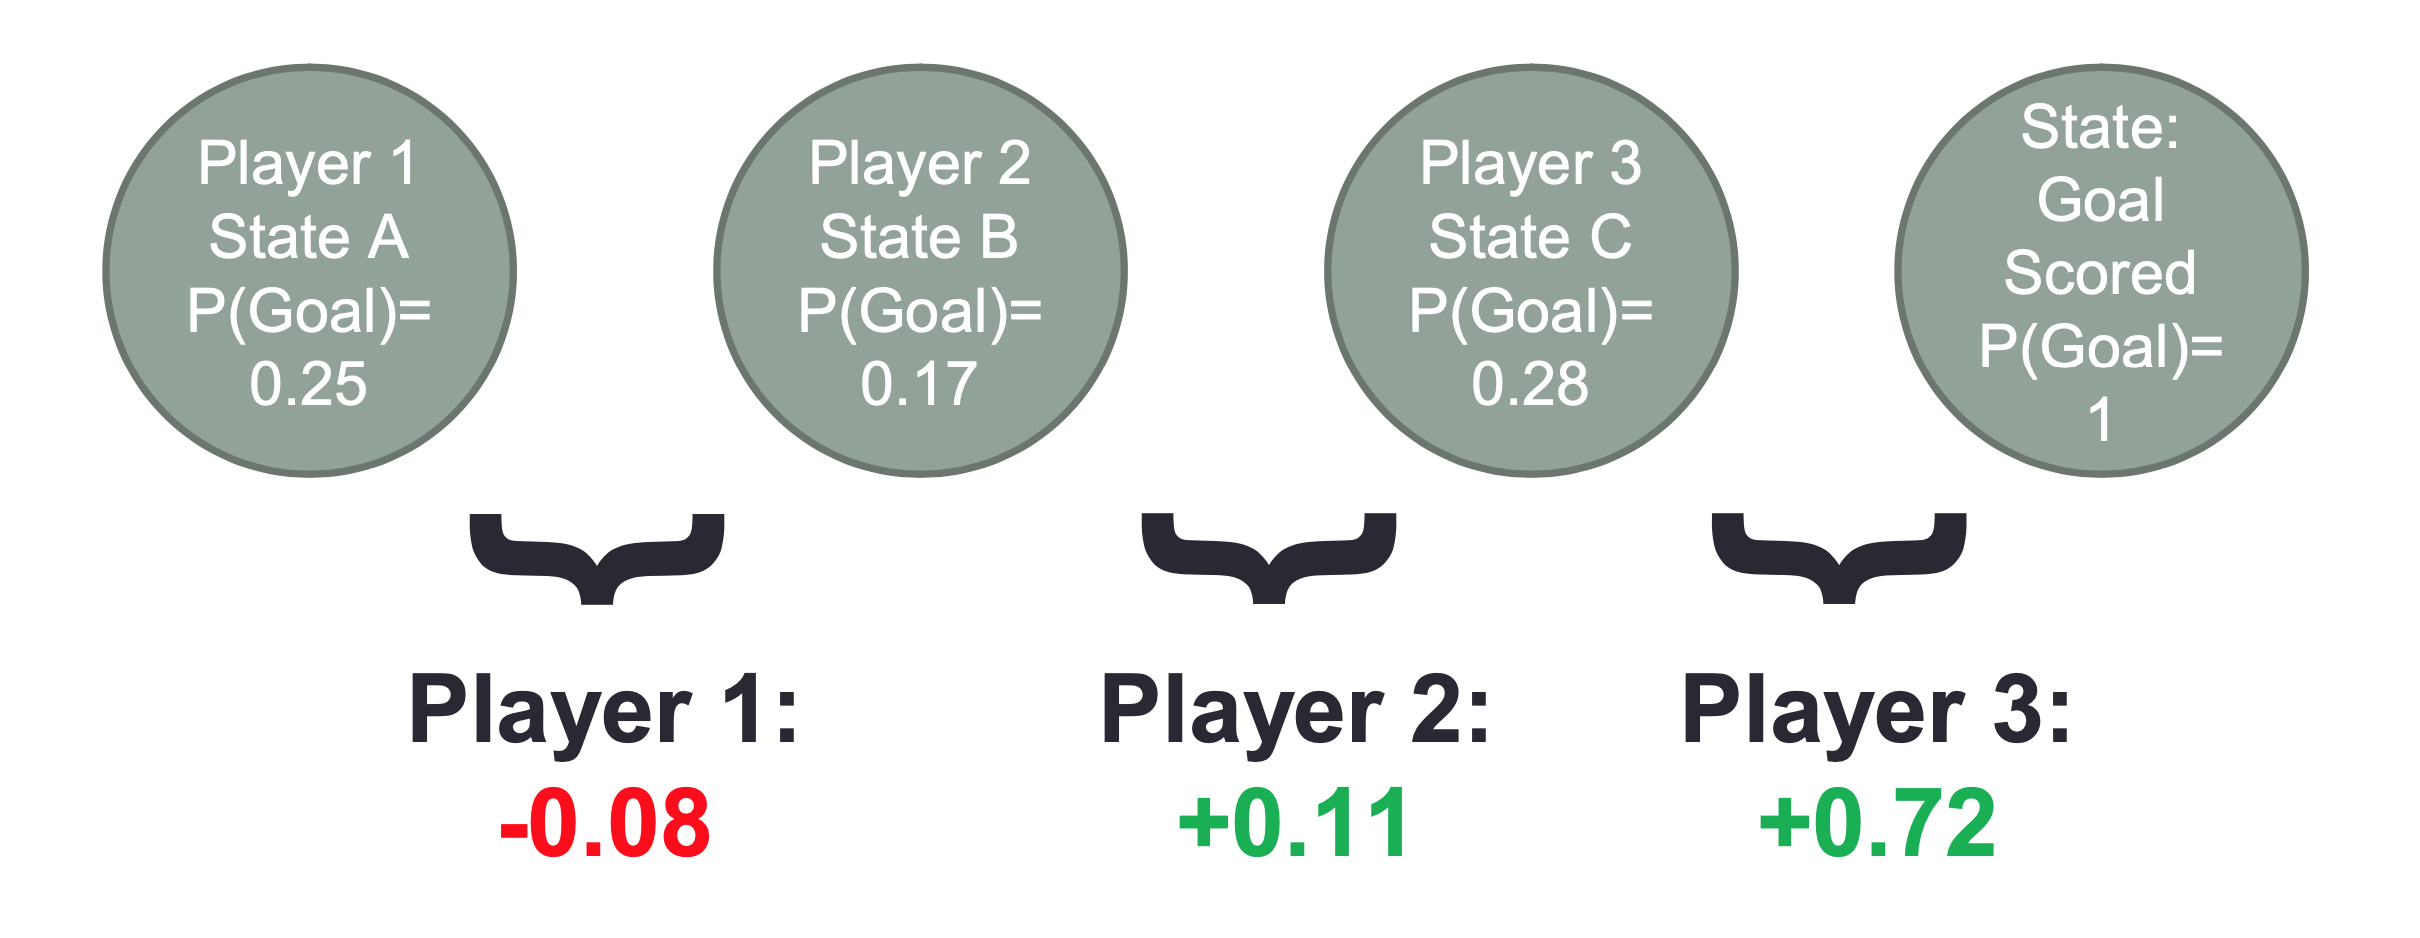
\includegraphics[scale=0.25]{images/ruddchain1.png}
        \caption{Possession chain leading to a goal.}
        \label{fig:syn1}
    \end{subfigure}
    
    \begin{subfigure}[b]{0.75\textwidth}
        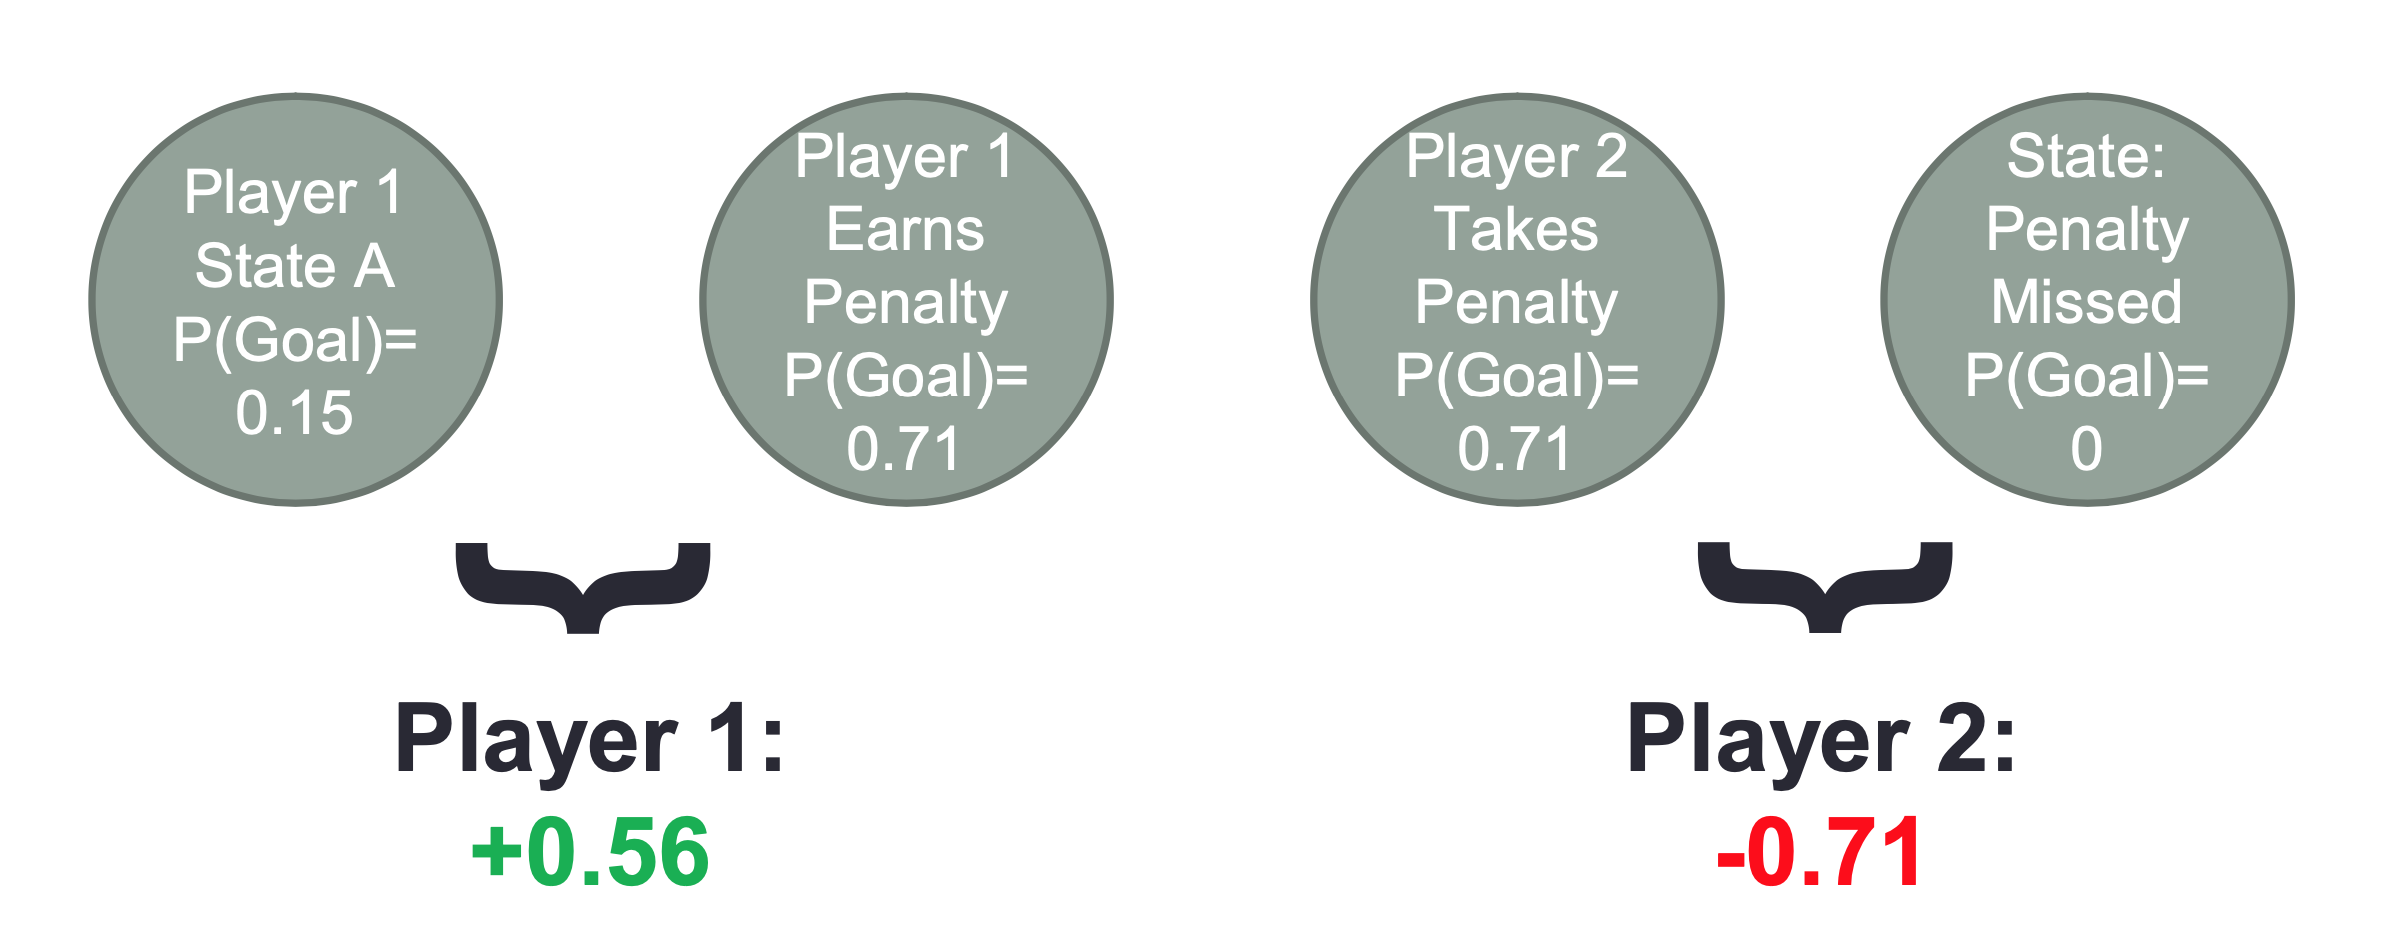
\includegraphics[scale=0.25]{images/ruddchain2.png}
        \caption{Possession chain leading to a loss of possession.}
        \label{fig:syn2}
    \end{subfigure}
    
    \caption{Simple examples of possessions as Markov chains by Rudd \cite{rudd1}. In a) the first transition decreases the probability of scoring and the player is penalised. The next transition increases the probability of scoring, and the player responsible is rewarded. The third transition is into a 'goal' state, indicating that player 3 scored. Player three is heavily credited. In b), a player wins a penalty - a set piece with a very high probability of a goal being scored. Player 2 takes the penalty and misses, and is heavily penalised.}
    \label{fig:synthetic}
\end{figure}

Rudd's framework allowed analysts to assign credit more fairly for a goal, or even a goal-scoring opportunity, and distinguish simple, ineffective passes from the important ones. It also gave rise to the notion of "non-shot" metrics in football. Rudd was promptly hired by StatDNA, which was bought by Arsenal F.C. in 2014 \cite{guar1}. 

\subsection{StatsBomb's \textit{Ball Progression Model} (2019)}

In 2019, football analytics company StatsBomb released an article on their website announcing a new "possession based Markov model" which they called their \textit{Ball Progression Model}, an extension of Rudd's 2011 framework \cite{sbomb2}. Using improved (since 2011) techniques and their far richer data set, StatsBomb extended Rudd's model to include a total of 84 transient states and two absorbing states (goal and loss of possession). 

Running the model on data captured from Europe's top five leagues confirmed that the states most likely to produce goals were front-and-center of the opposition's goal. Perhaps less intuitively, it revealed that teams are most likely to lose possession in the corners either side of their own goal area.

With the probabilities of a goal being scored mapped to each of the states, the model can then be used to assess player performance, based on their contribution - the relative increase (or decrease) in the probability of a goal being scored as a result of the transition they caused (by passing, dribbling etc.), as illustrated in \textbf{Fig. \ref{fig:sbbpm}}.

\begin{figure}[h]
    \centering
    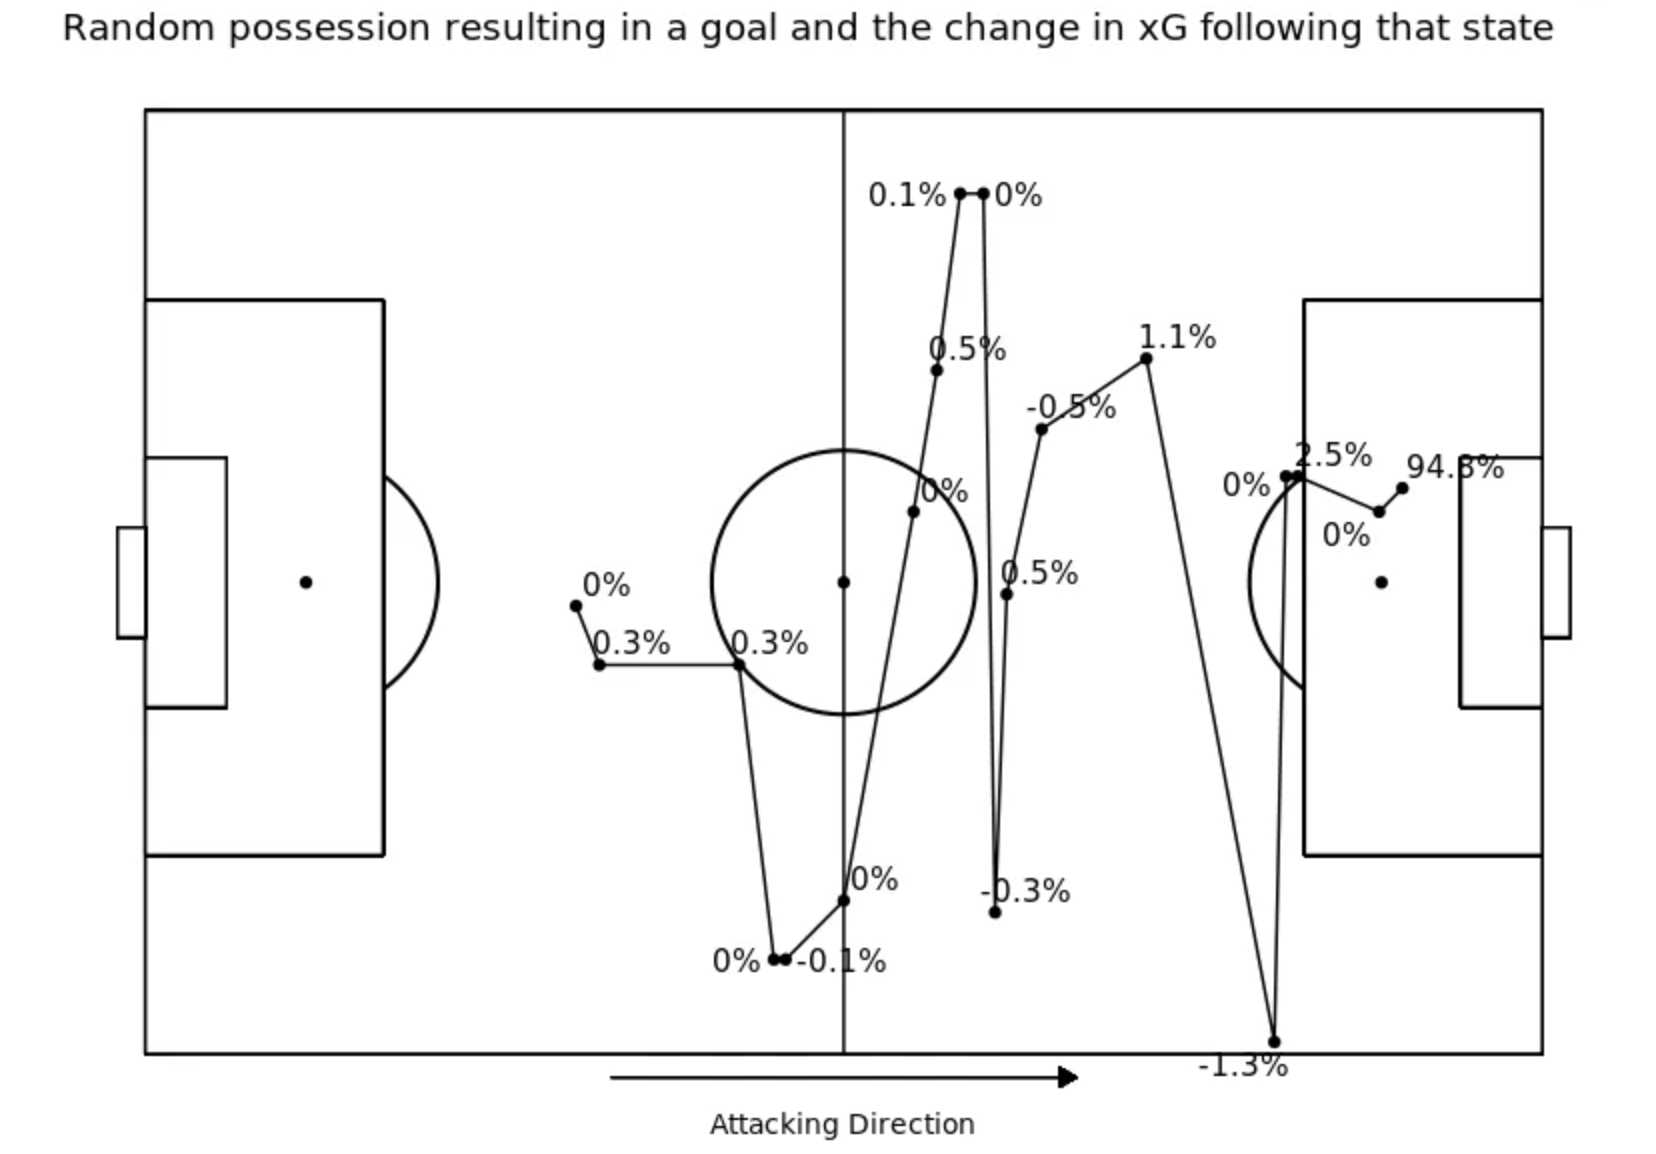
\includegraphics[scale=0.4]{images/bpm.png}   
    \caption{Randomised possession chain showing the relative increase and decrease in the probability of a goal being scored in each state, generated by StatsBomb using their Ball Progression Model \cite{sbomb2}. The final touch increases the probability by 94.8\% to 1 - indicating that a goal is scored.}
    \label{fig:sbbpm} 
\end{figure}

Of particular interest is StatsBomb's discussion of the suitability of Markov models for reasoning about chains of possession in football. While recognising that they provide a useful abstraction, and produce reasonable results, the following limitations are highlighted:

\begin{itemize}
    \item \textit{"...Markov models assume the “memoryless” property when in reality a soccer possession is not memoryless. The probability of scoring when you are in a current state can depend on previous passes and carries leading up to the current state."}
    \item \textit{"...this simple Markov model does not consider the action required to transition between states. For instance,  the probability of a possession resulting in a goal may be different given that you passed into a zone vs. dribbled into a zone."}
    \item \textit{"...perhaps the most obvious limitation of this Markov model is the categorized structure of transient and absorption states. This causes the loss of information and limits applications especially in the free-flowing game of football."} \cite{sbomb2}
\end{itemize}

To address these limitations, StatsBomb suggest future work on an improved model, involving Markov decision processes and higher-order Markov models (in which a model of $n$-th order has states with transition probabilities that depend on the previous $n$ states). The results of this work are proprietary and therefore cannot be summarised here.

\subsection{Strategy Synthesis for Autonomous Agents using PRISM (2018)}

In this published research by Giaquinta \textit{et al.} \cite{fac2}, the authors first provide a concise summary of Markov decision processes and the PRISM model checker. The paper then details a number of models, of increasing complexity, representing a series of scenarios, \textit{"inspired by realistic situations for a range of autonomous vehicle applications, e.g. border patrol using autonomous vehicles, exploration of unexplored terrain, and search and rescue operations."} The paper investigates the viability of automatically generated controllers for these autonomous systems.

The PRISM model checker is used to verify the models and generate \textit{optimal strategies}, minimising mission times and scheduling recharge stops for autonomous agents with a variety of battery capacities. The paper clearly demonstrates PRISM's ability to synthesise the optimal strategy across all non-deterministic choices, which can be reconstructed as a DTMC in PRISM for further analysis. 

The authors highlight the need for abstraction techniques which minimise the state space of modelled systems, as well as some \textit{quality-of-life} improvements that would make strategy synthesis in PRISM less laborious. 

The paper sets out an approach to strategy generation that strongly influences the work carried out in this project.

\subsection{Other Related Work}

\textbf{Twelve Football (Sumpter, 2017)}: In a blog post in 2017, David Sumpter announced that he had been developing an automated tool for evaluating player performance based on every on-the-ball event recorded during a match \cite{sump2}. The tool was made available online as part of the football analytics package \textit{Twelve}  \cite{twel1}. The implementation uses machine learning, but the basis for evaluation is a Markov model derived from captured match data. 

\begin{figure}[h]
    \centering
    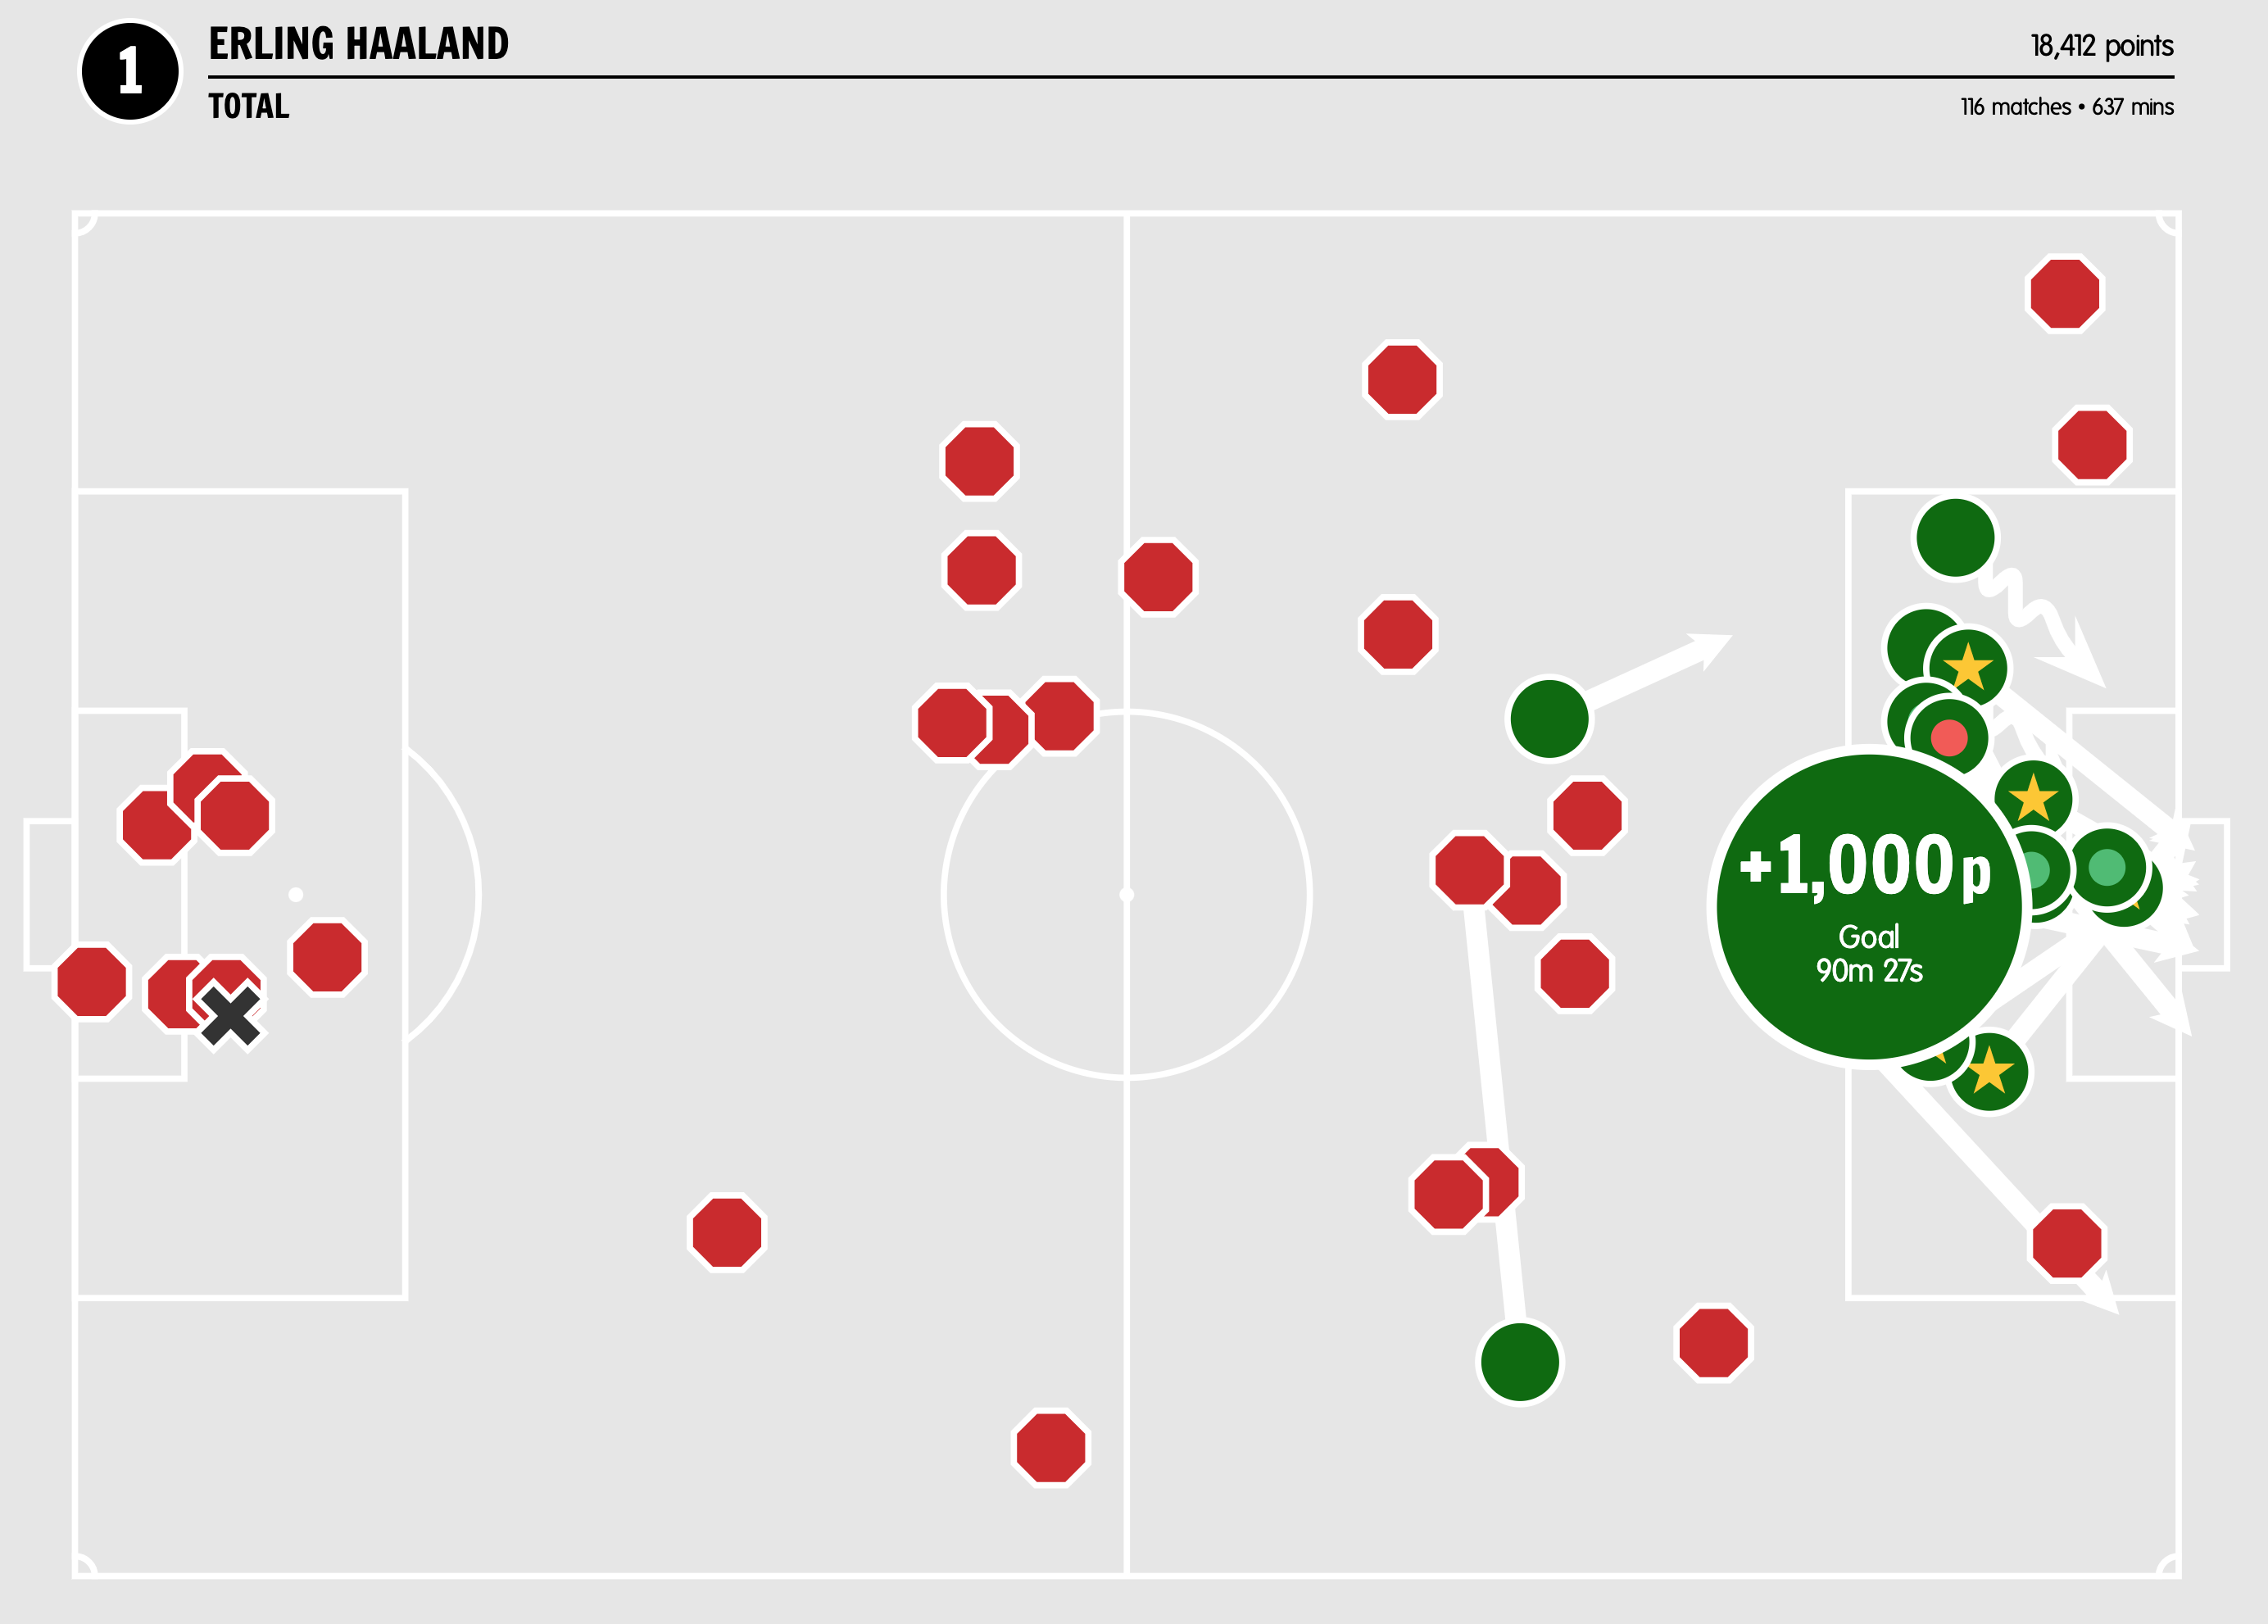
\includegraphics[scale=0.2]{images/twelve2.png}   
    \caption{Twelve Football's auto-generated pitch view of Erling Haaland's most important touches during the 2020-21 UEFA Champions' League campaign \cite{twel1}. The tool is interactive, allowing users to highlight each event to discover its type and value.}
    \label{fig:twel} 
\end{figure}

\textbf{xT: Expected Threat (Singh, 2019)}: In a self-published blog post \cite{ksing1}, Karun Singh detailed the motivatiions and theory behind a new non-shot metric called \textit{expected threat}, or xT. The objective, once again, was to better apportion credit to players in a move that leads to goal. The core idea is similar to Rudd's approach of rewarding players for actions which increase the probability of a goal being scored, but with more detailed spatial data (Singh defines 192 zones across the entire pitch). The article also contains a number of interactive tools and visualisations, evaluating the cumulative xT created over the 2017-18 English Premier League season on a  per-team and per-player basis.

\textbf{Model checking for detection of sport highlights (Bertini \textit{et al.}, 2003)}: The most relevant (to this study) application of model checking identified was a 2003 paper on the use of \textit{"finite state machine models and model checking as a general and effective approach to model sports highlights and detect their occurrence automatically, from the analysis of the video visual cues"} \cite{bert1}. Video analysis techniques are shown to be capable of identifying game states and sequences of events. Constraints are evaluated as the footage progresses, and if satisfied, the state advances towards being a confirmed `highlight' that would be suitable for a televised summary package. Similar techniques could be of value in gathering football data for possession models. However, the model checking contribution is largely inconsequential to this study.

% What did other people do, and how is it relevant to what you want to do?

%==================================================================================================================================
\chapter{Modelling Football}\label{limits}

The majority of previous work identified is primarily concerned with evaluating the contributions of individual players. Our aim, broadly, is to identify patterns of play that can increase the likelihood of goals being scored, using model checking. To achieve this, we must first construct appropriate models from the data available to us.

In order to evaluate the potential of probabilistic model checking for strategy generation, we propose the use of simplified models, both in order to facilitate quicker evaluation and iteration, and as a necessity of the limited data available. The possession models constructed for this study are subject to the following limitations:

\begin{itemize}
    \item only attacking contributions, which we define as actions in the opposition's half, are considered;
    \item only transitions arising from actions which are classified as passes or shots are included;
    \item we have removed data about set pieces, which have been shown to have very different probabilities from open play \cite{rudd1};
    \item there is no off-the-ball data to indicate defensive positions of opposition players; therefore, states defined are solely based upon pitch location (and xG).
\end{itemize}

\section{The Data}\label{data}

The data used to build our models was collected by Wyscout \cite{wysc1} and published alongside a paper by Pappalardo \textit{et al.} \cite{data1} examining the data set and its general usefulness for research in data science. The authors describe the data as \textit{"the largest open collection of soccer-logs ever released."}

The various data are divided between JSON (JavaScript Object Notation) files. Each collection of files provides information about teams, referees, competitions, etc.; our model is constructed from the 'events' data sets. These comprise every on-the-ball event from every match played in the 2017-18 seasons of La Liga (Spain), Serie A (Italy), 1. Bundesliga (Germany), Ligue 1 (France) and the Premier League (England). Additionally, the same data is included for the UEFA European Football Championship 2016 and the FIFA World Cup 2018, both of which are international tournaments. As the format of these competitions differs from that of the domestic leagues, we have chosen to exclude them from our data for the sake of consistency.

The following summary (reproduced from the paper by Pappalardo \textit{et al.}) lists the fields present in an event object:

\begin{itemize}
    \item \texttt{eventId}: the identifier of the event’s type. Each \texttt{eventId} is associated with an event name (see next point);

    \item \texttt{eventName}: the name of the event’s type. There are seven types of events: pass, foul, shot, duel, free kick, offside and touch;

    \item \texttt{subEventId}: the identifier of the subevent’s type. Each \texttt{subEventId} is associated with a subevent name (see next point);

    \item \texttt{subEventName}: the name of the subevent’s type. Each event type is associated with a different set of subevent types;

    \item \texttt{tags}: a list of event tags, each describing additional information about the event (e.g., accurate). Each event type is associated with a different set of tags.

    \item \texttt{eventSec}: the time when the event occurs (in seconds since the beginning of the current half of the match);

    \item \texttt{id}: a unique identifier of the event;

    \item \texttt{matchId}: the identifier of the match the event refers to. 

    \item \texttt{matchPeriod}: the period of the match. It can be “1H” (first half of the match), “2H” (second half of the match), “E1” (first extra time), “E2” (second extra time) or “P” (penalties time);

    \item \texttt{playerId}: the identifier of the player who generated the event.

    \item \texttt{positions}: the origin and destination positions associated with the event. Each position is a pair of coordinates (x, y). The x and y coordinates are always in the range [0, 100] and indicate the percentage of the field from the perspective of the attacking team. In particular, the value of the x coordinate indicates the event’s nearness (in percentage) to the opponent’s goal, while the value of the y coordinates indicates the event’s nearness (in percentage) to the right side of the field;

    \item \texttt{teamId}: the identifier of the player’s team. 

\end{itemize}

\begin{figure}[h]
    \centering
    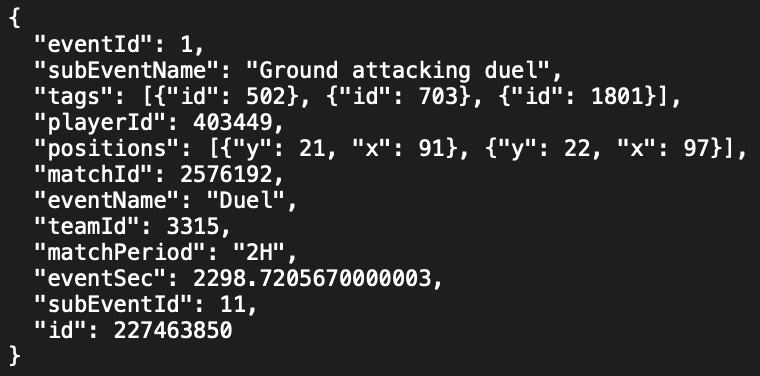
\includegraphics[scale=0.6]{images/json2.png}   
    \caption{A typical event entry.}
    \label{fig:json} 
\end{figure}

%The analysis chapter explains the process by which you arrive at a concrete design. In software 
%engineering projects, this will include a statement of the requirement capture process and the
%derived requirements.

%In research projects, it will involve developing a design drawing on
%the work established in the background, and stating how the space of possible projects was
%sensibly narrowed down to what you have done.

\section{Building an xG model}

\subsection{What is xG?}

Expected goals, commonly written as \textbf{xG}, is a measurement of \textit{shot quality}, based on the probability that a shot will result in a goal. An \textit{xG model} could be derived from something as simple as the ratio of goals scored to shots taken from a given area of the pitch.  

While the term appears in research published as early as 1993 \cite{xg901}, it is described in more familiar terms (though not by name) in a 2004 article by Ensum \textit{et al.}, where\textit{ "...distance and angle from goal, the degree of space from an opposition player, the number of players in front of goal and whether the shot originated from a cross"} were identified as key factors in evaluating shot quality \cite{ens04}. 

Modern, market-leading xG models are based on incredibly detailed data collected from many years of football. StatsBomb's model, for example, includes information such as the positions of defenders and goalkeepers, and which body part was used to take a shot. Since its most recent update, the model even accounts for the height of the ball when struck by an attacking player \cite{sbomb3}. 

For the purposes of this investigation, we define a simple xG model based on the Wyscout data, which relies solely on the spatial information found in the \texttt{positions} field of event records.

\subsection{Modelling xG with Python}\label{xgsection}

Using techniques outlined in the \textit{Mathematical Modelling of Football} course \cite{upps1} developed by Sumpter \textit{et al.} and made available by Uppsala University, we can develop our own xG model. In doing so, we make use of various python libraries which provide useful functionality for managing and modelling data, including \textit{pandas} \cite{pand1}, \textit{NumPy} \cite{nump1}, \textit{Matplotlib} \cite{matp1} and \textit{statsmodels} \cite{stat1}. The source code for this model and its visualisations can be found at \texttt{/code/python/buildxG.py} in the repository that accompanies this paper.

\begin{figure}[htb] 
    \centering
    \begin{subfigure}[b]{0.45\textwidth}
        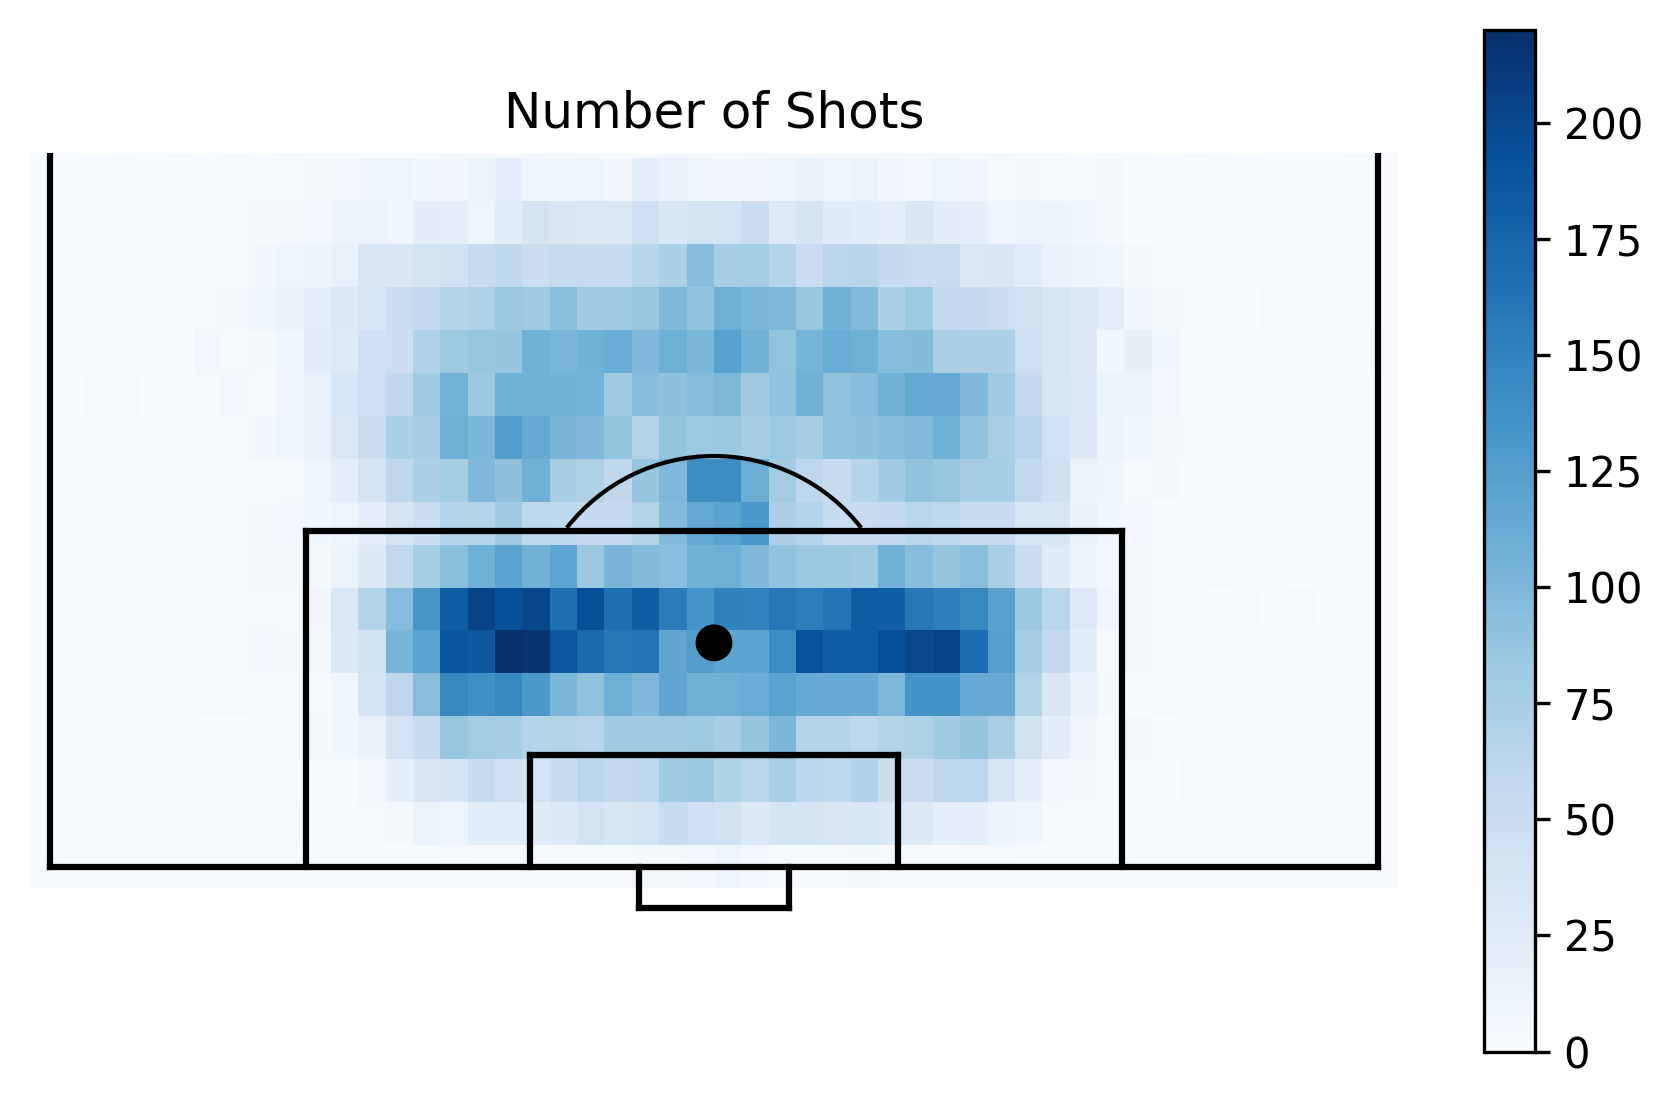
\includegraphics[width=\textwidth]{images/shotplot.png}
        \caption{2-dimensional histogram of locations from which shots were taken.}
        \label{fig:splot}
    \end{subfigure}
    ~
    \begin{subfigure}[b]{0.45\textwidth}
        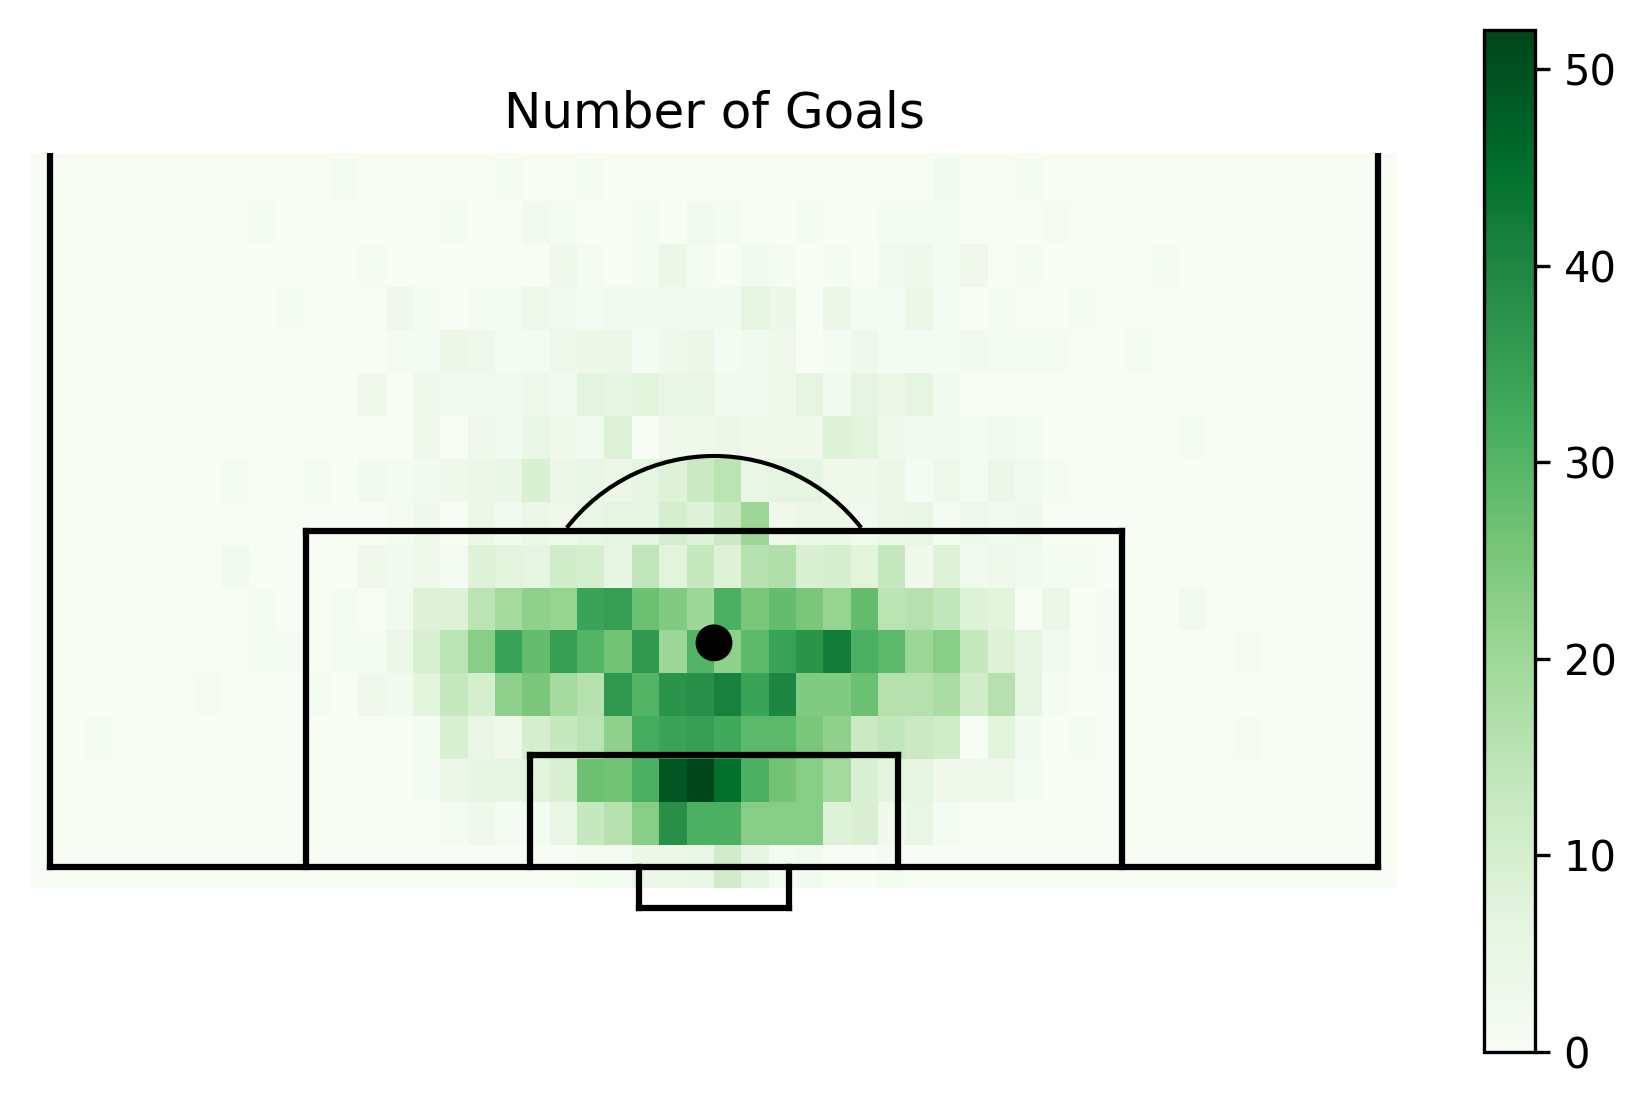
\includegraphics[width=\textwidth]{images/goalplot.png}
        \caption{2-dimensional histogram of locations from which goals were scored.}
        \label{fig:gplot}
    \end{subfigure}
    ~   
    \caption{2-dimensional histograms built from shot and goal data. \subref{fig:splot} shows locations from where shots were taken (i.e. the ball was deliberately kicked towards goal), with darker blue indicating a greater concentration of shots. \subref{fig:gplot} shows those shots which resulted in goals, with a darker green indicating a greater concentration of successful shots. These figures show that more goals are scored from advanced, central positions - in other words, within the opposition's box.
    }\label{fig:histo1}
\end{figure}

\begin{figure}[h]
    \centering
    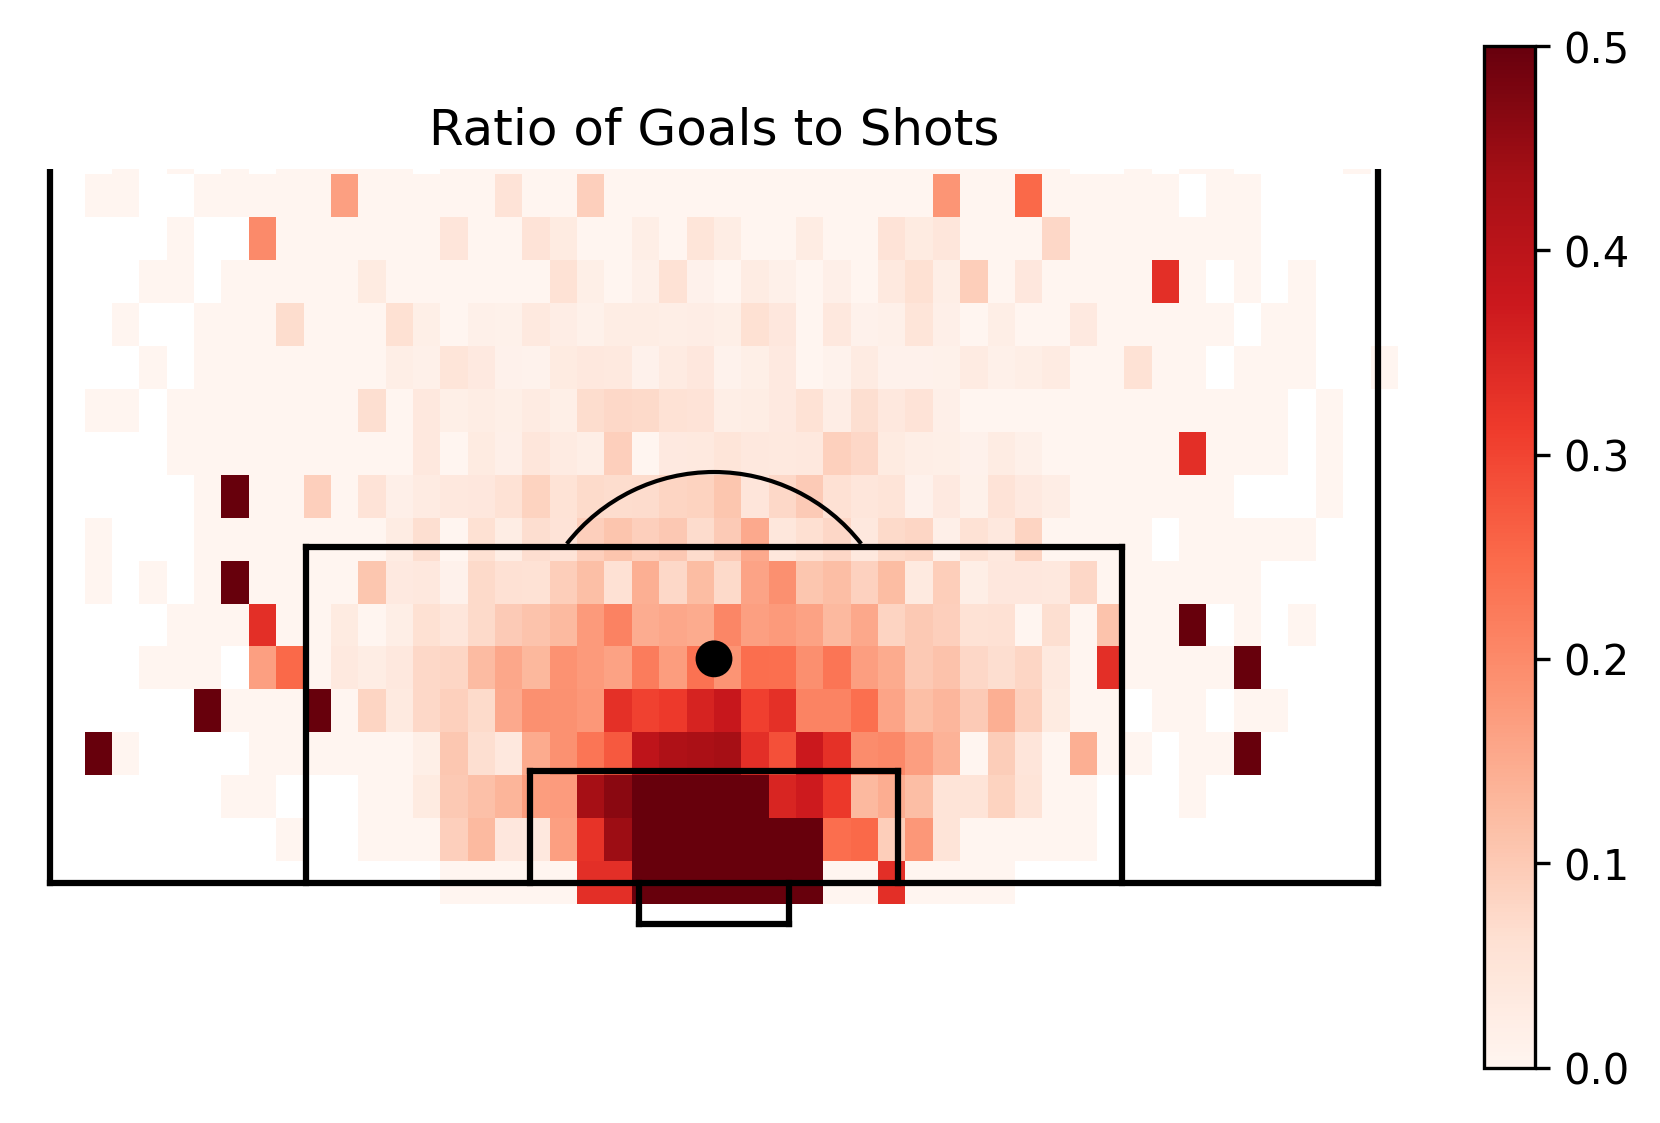
\includegraphics[scale=0.6]{images/xgplot1.png}   
    \caption{2-dimensional histogram of pitch locations with a high goals-to-shots ratio. Outlying areas with a high ratio are a result of a handful of long-range goals scored from areas where very few shots are taken.}
    \label{fig:xg1} 
\end{figure}

We begin by extracting those events which have been classed as shots from the data set. Using the coordinates recorded for each shot, we can plot a 2-dimensional histogram, with pitch markings overlaid for context. We can generate a similar histogram for shots which resulted in goals. Both are shown in \textbf{Fig. \ref{fig:histo1}}. Anyone familiar with football will not be surprised to see a concentration of shots in and around the box, with a greater degree of success closer to goal.

As stated previously, a simple xG model can be constructed simply by taking the ratio of goals to shots. We can generate a third histogram from simple arithmetic - a point-to-point division of the number of goals by the number of shots - which begins to give us an idea of the areas of the pitch with a high probability of goals being scored. 

\textbf{Fig. \ref{fig:xg1}} confirms that proximity to goal is an important factor in xG. Within the smaller internal box, known as the six-yard box, the histogram indicates a probability of 0.5 that a shot will result in a goal - somewhat generous when compared to more sophisticated models \cite{sump1} Additionally, we can see a clustering of high xG values closer to the middle. This demonstrates the value of what Ensum \textit{et al.} referred to as the "angle from goal," the angle formed at the shot location with respect to both goal posts (\textbf{Fig. \ref{fig:angles}}).

\begin{figure}[htb] 
    \centering
    \begin{subfigure}[b]{0.45\textwidth}
        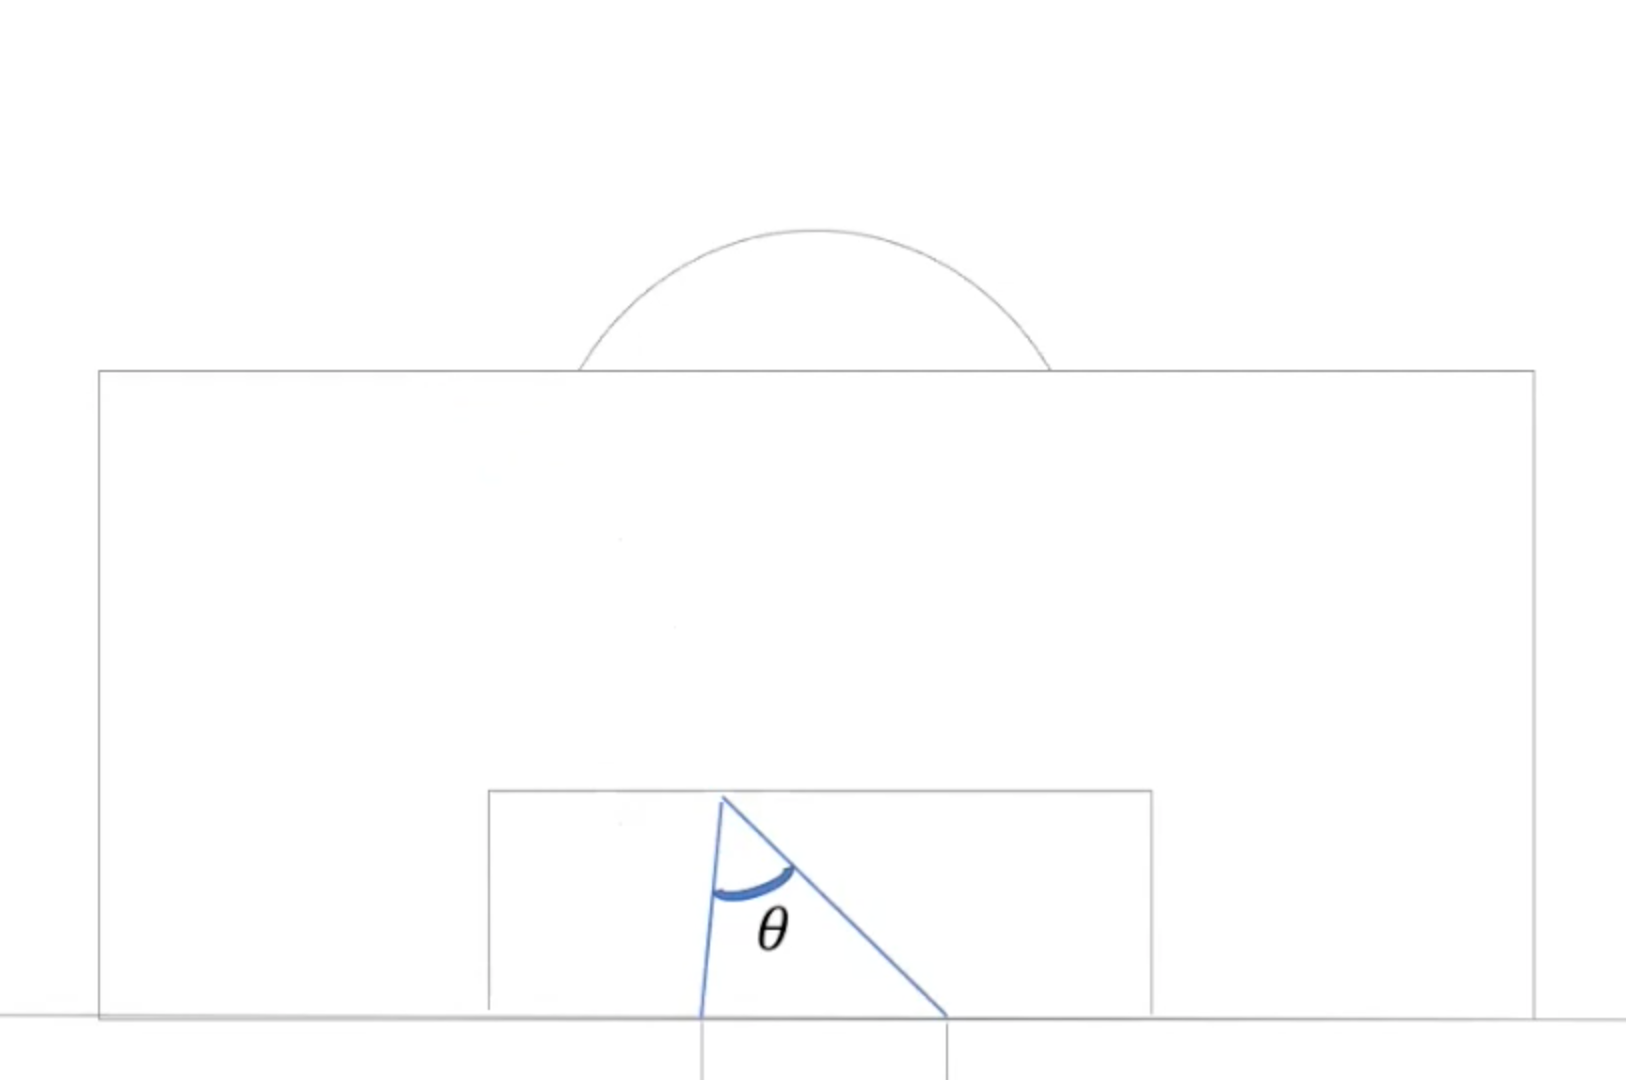
\includegraphics[width=\textwidth]{images/wideangle.png}
        \caption{Example of a large "angle from goal."}
        \label{fig:bigang}
    \end{subfigure}
    ~
    \begin{subfigure}[b]{0.45\textwidth}
        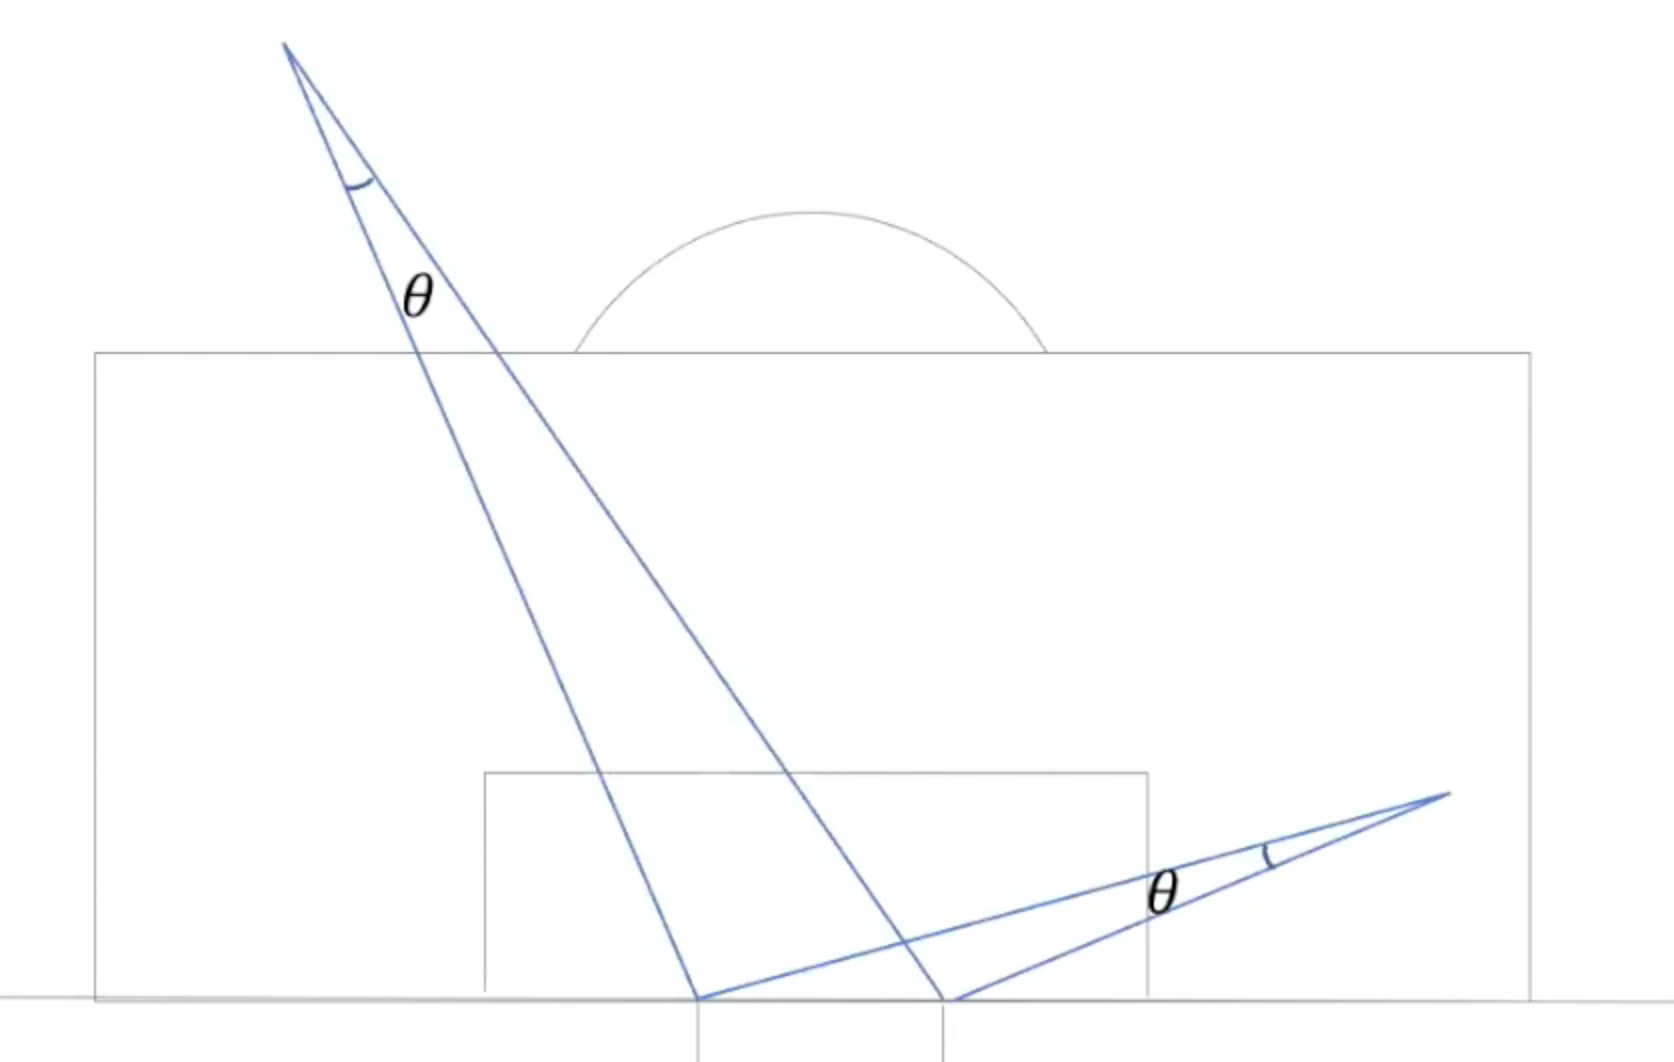
\includegraphics[width=\textwidth]{images/tightangle.png}
        \caption{Examples of a small "angle from goal."}
        \label{fig:smallang}
    \end{subfigure}
    ~   
    \caption{Diagrams showing the angle concerned when evaluating shot quality. \subref{fig:smallang} demonstrates the influence of distance on the size of this angle.}
    \label{fig:angles}
\end{figure}

There are, however, some outlying areas in our histogram with a high probability of scoring, which to a football fan would appear anomalous. These arise because goals \textit{are} scored from these areas, but very infrequently. Our model indicates that these areas have a high xG, but this is because we have a very small sample of shots taken from these areas. Our model needs further refinement.

\begin{figure}[h]
    \centering
    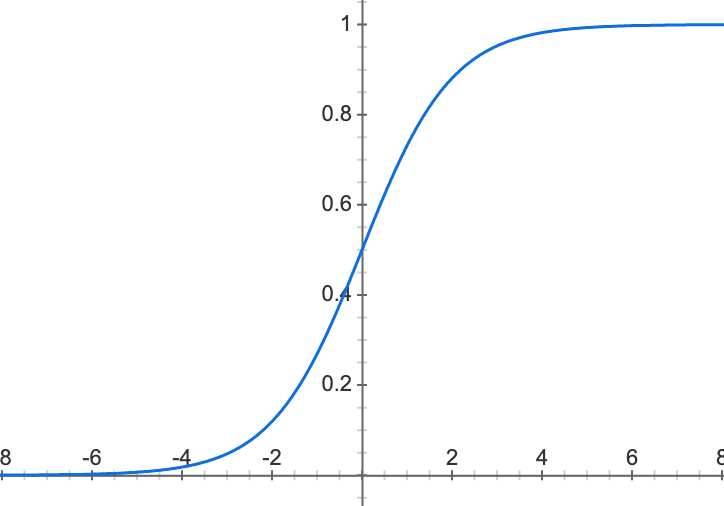
\includegraphics[scale=0.6]{images/logistic.png}   
    \caption{Graph of a standard logistic function. The asymptotes towards $y=0$ and $y=1$ make the function useful for modelling probabilities.}
    \label{fig:logcurv} 
\end{figure}

Our next model makes use of a statistical method called \textit{logistic regression}. A standard logistic function takes the form:

\[ f(x) = \frac{1}{1 + e^{-x}} \]

When graphed, this function produces a \textit{sigmoid curve} in which all values of $y$ lie within the interval $(0,1)$ (\textbf{Fig. \ref{fig:logcurv}}). This property means that the logistic curve is very useful when modelling probabilities, which will always be between 0 and 1. 

We begin with a single-variable model which examines the likelihood of scoring based on the angle from goal. The points plotted in \ref{fig:fitt1} show the probabilities of scoring, calculated previously, as a function of the angle from which a shot is taken. The process of logistic regression aims to 'fit' a logistic curve to the data points such that the log-likelihood is minimised, giving us a smooth, continuous function by which we can map "angle from goal" to xG values.

\begin{figure}[htb] 
    \centering
    \begin{subfigure}[b]{0.45\textwidth}
        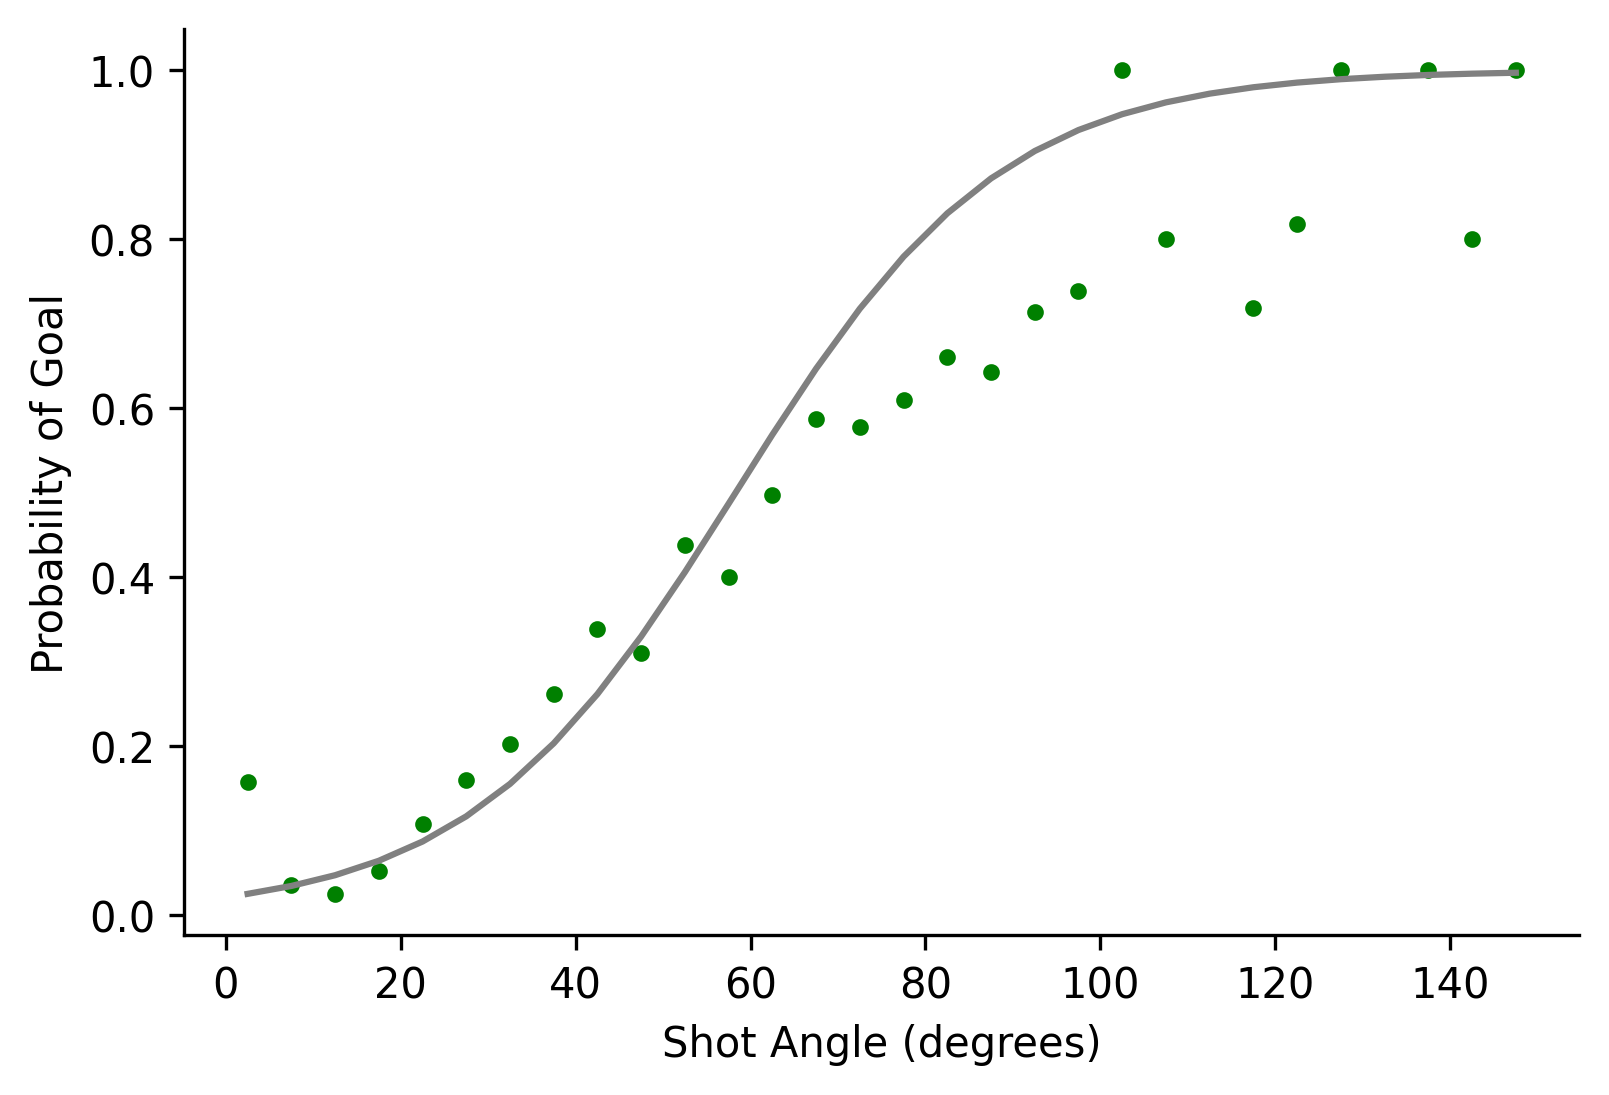
\includegraphics[width=\textwidth]{images/anglefit.png}
        \caption{A logistic curve fitted to a graph of xG as a function of shot angle.}
        \label{fig:angfit}
    \end{subfigure}
    ~
    \begin{subfigure}[b]{0.45\textwidth}
        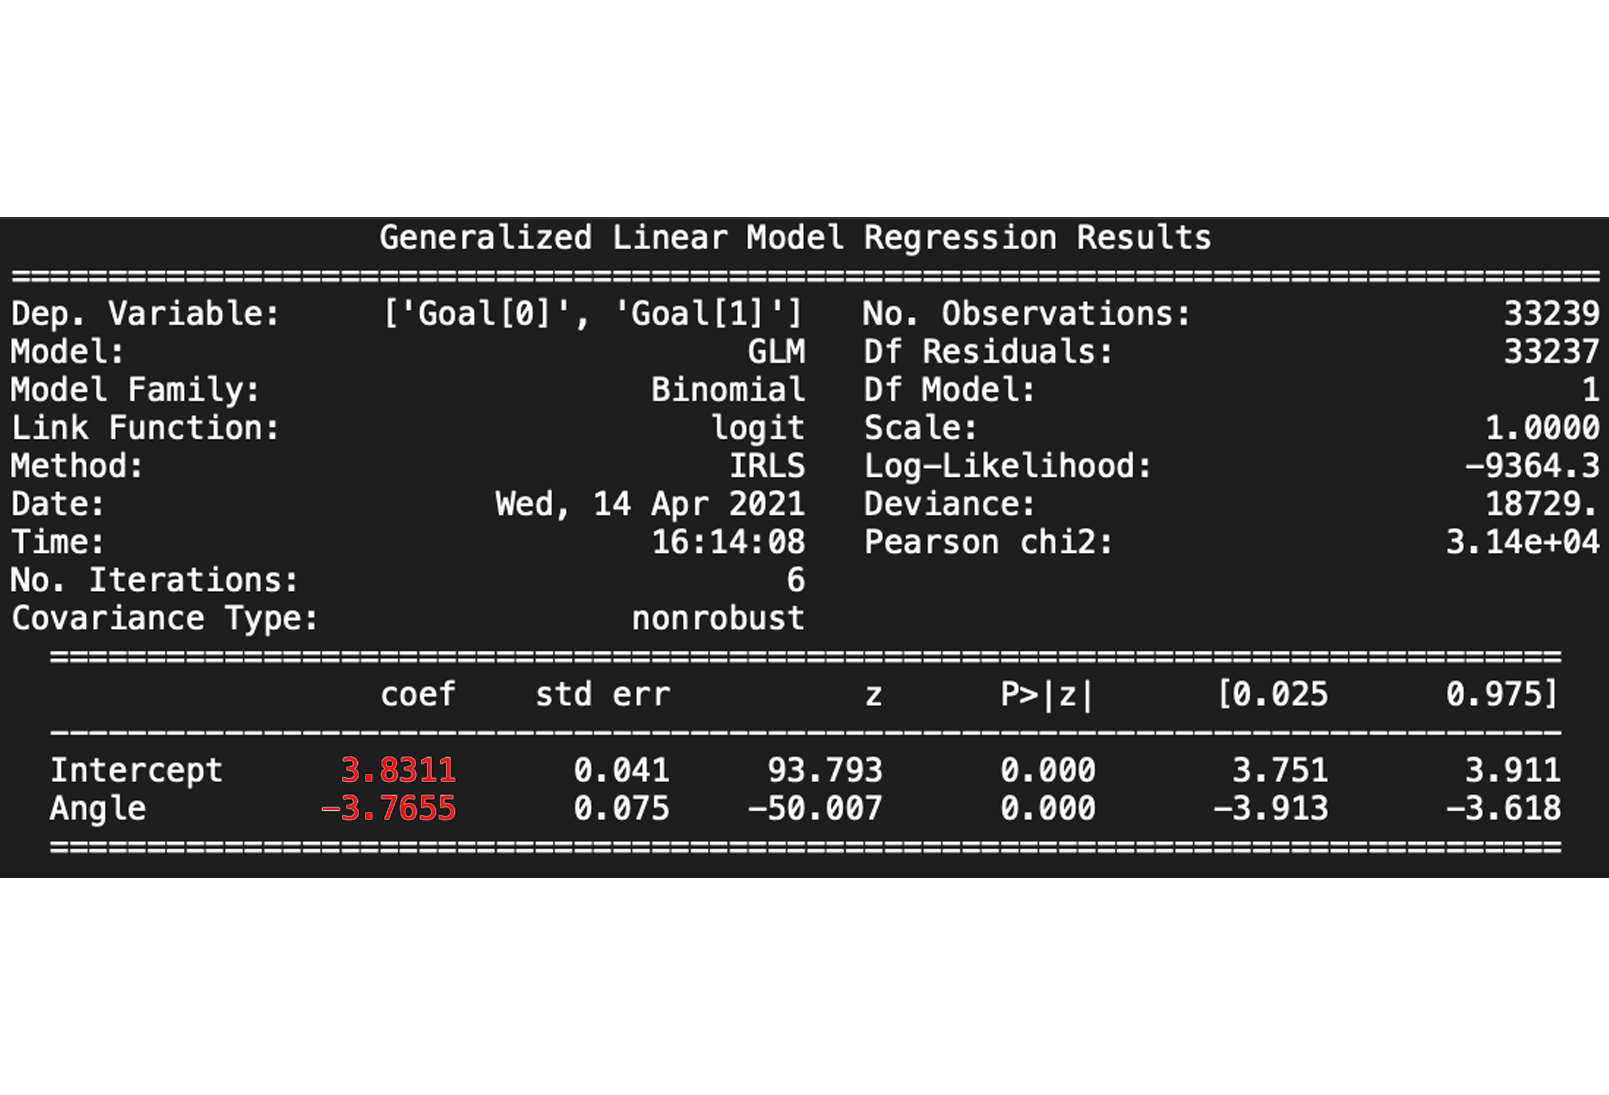
\includegraphics[width=\textwidth]{images/statsmodeloutput.png}
        \caption{Console output from the Python library statsmodel.}
        \label{fig:smout1}
    \end{subfigure}
    ~   
    \caption{\subref{fig:angfit} shows our xG graphed as a function of shot angle (green points). The Python library statsmodel fits a curve to the data using logistic regression. \subref{fig:smout1} shows the report generated by statsmodel. The fit is achieved by finding coefficients for intercept and angle (highlighted in red) which minimise log-likelihood.}
    \label{fig:fitt1}
\end{figure}

Similarly, we can plot xG as a function of distance from goal, and use \textit{statsmodel} to fit a curve to the data. Once again, we are left with a smooth, continuous function that lets us map distances to xG.

\begin{figure}[htb] 
    \centering
    \begin{subfigure}[b]{0.45\textwidth}
        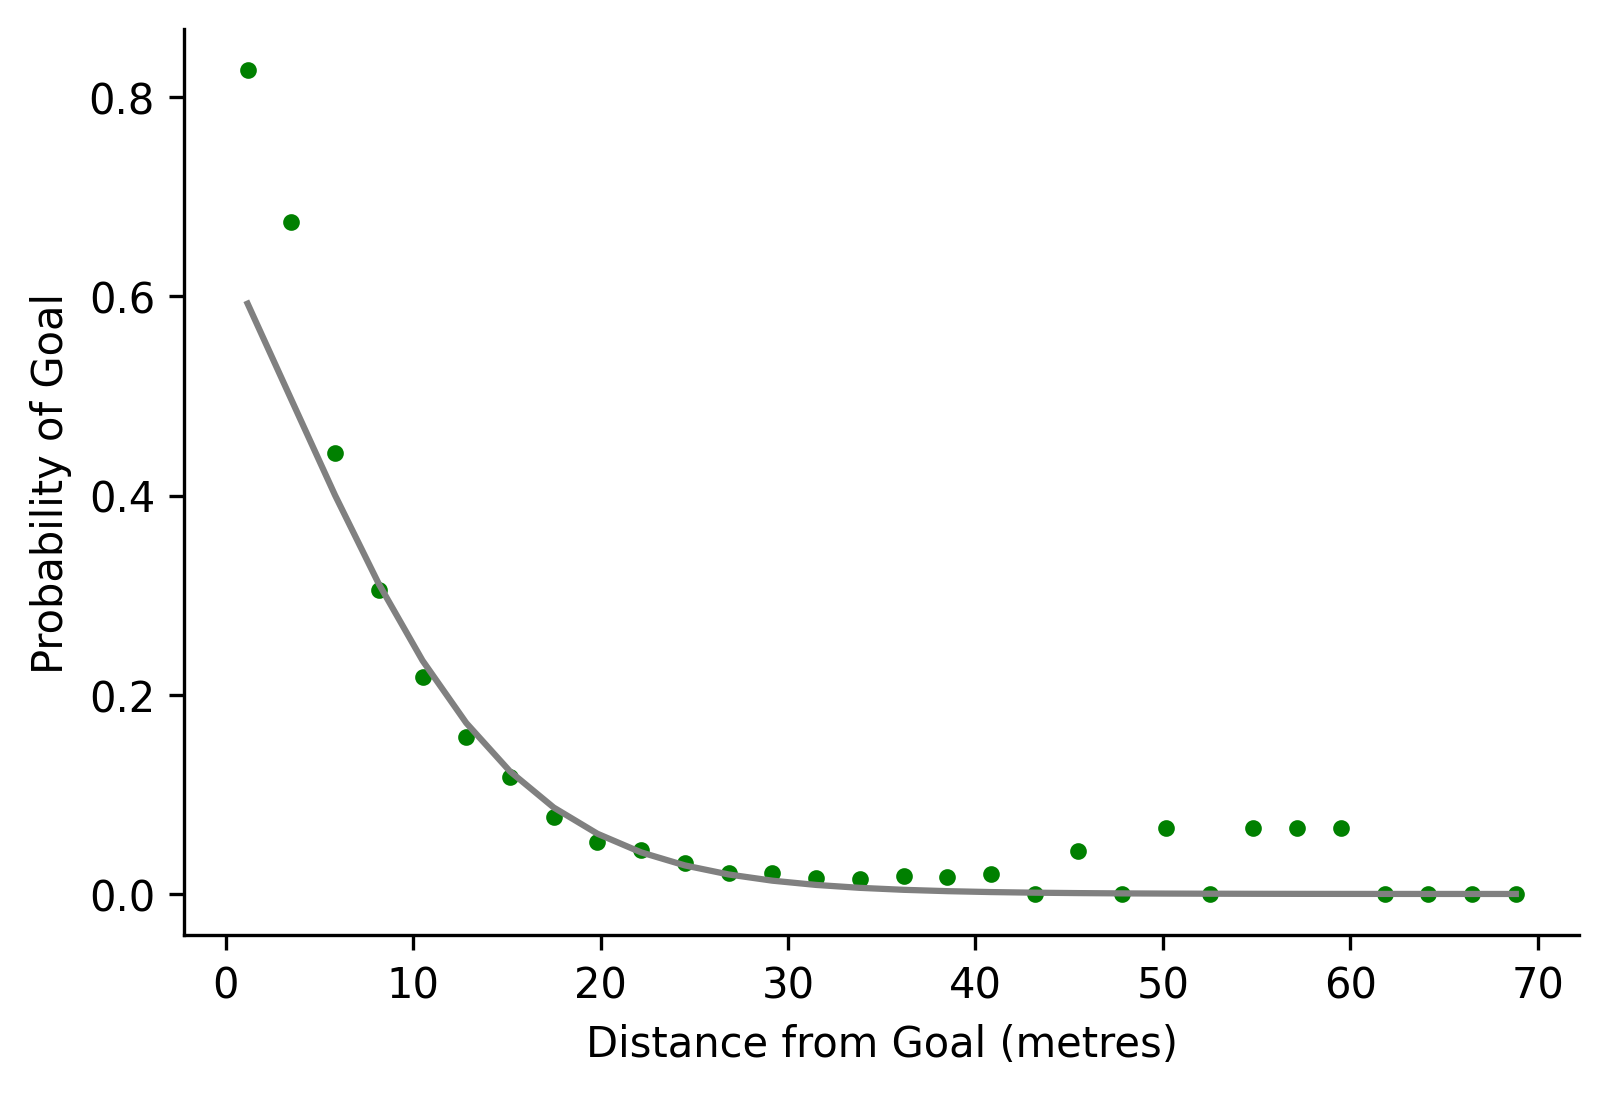
\includegraphics[width=\textwidth]{images/distfit.png}
        \caption{A logistic curve fitted to a graph of xG as a function of shot distance.}
        \label{fig:disfit}
    \end{subfigure}
    ~
    \begin{subfigure}[b]{0.45\textwidth}
        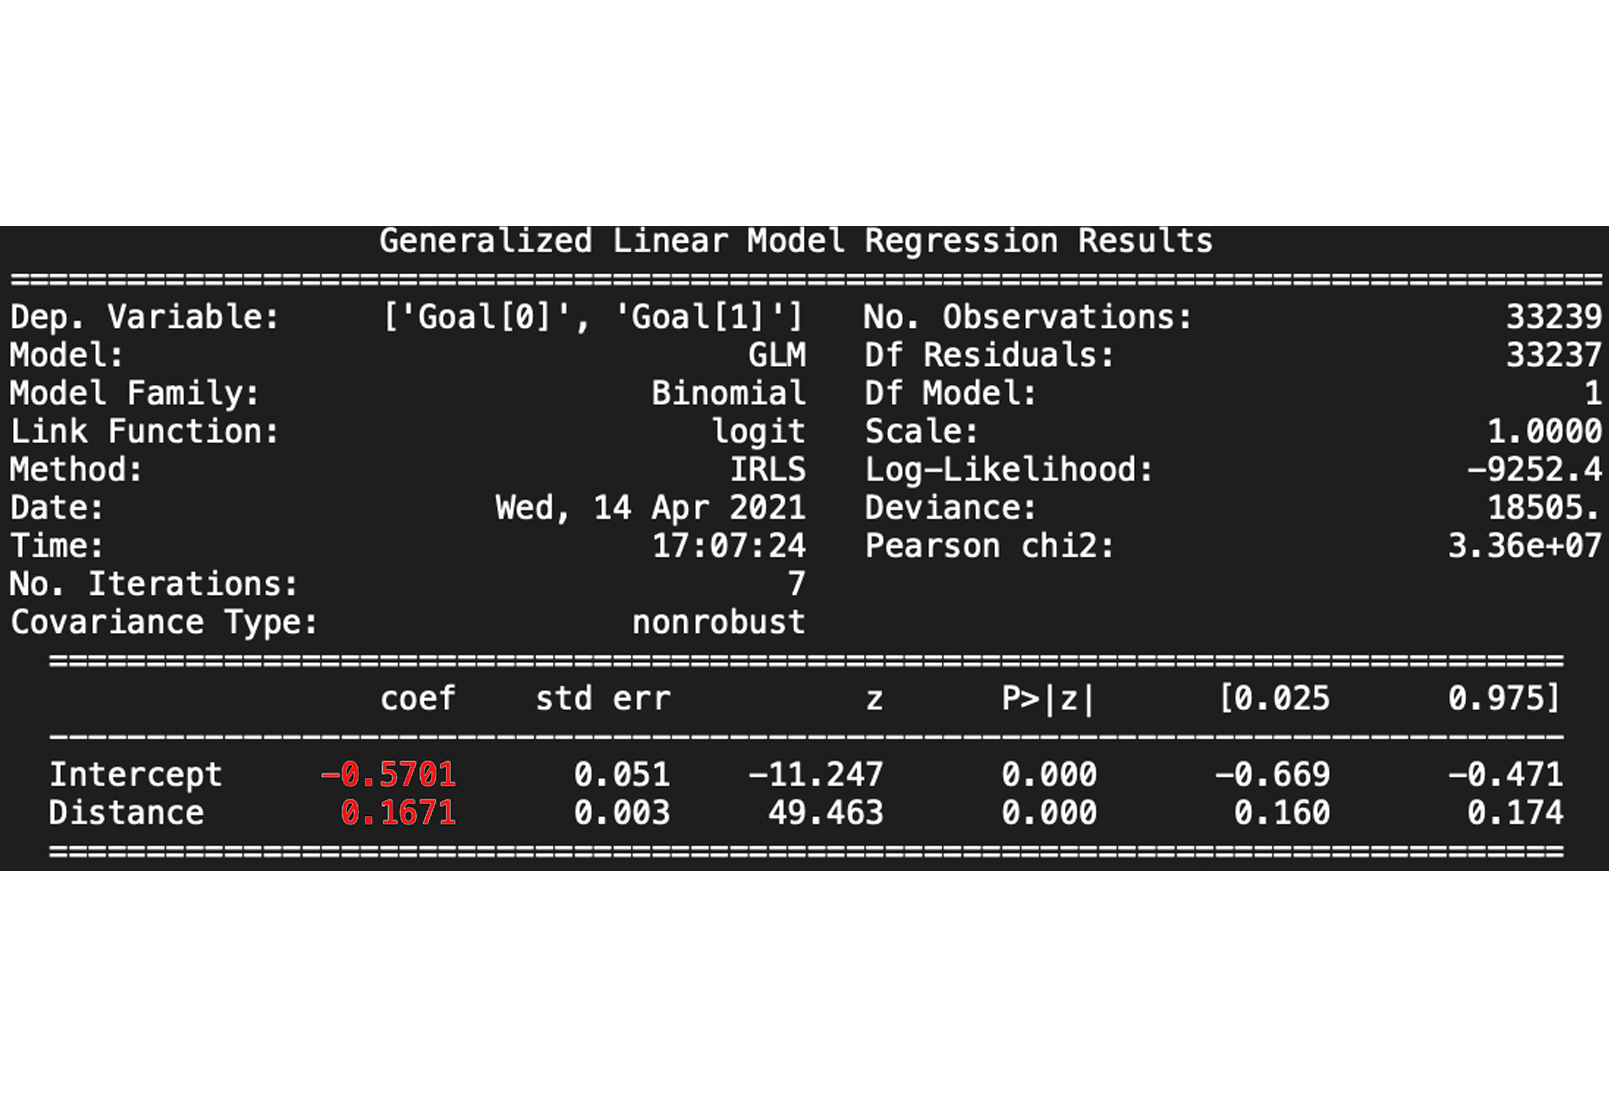
\includegraphics[width=\textwidth]{images/statsmodeloutput2.png}
        \caption{Console output from the Python library statsmodel.}
        \label{fig:smout2}
    \end{subfigure}
    ~   
    \caption{\subref{fig:angfit} shows our xG graphed as a function of shot distance (green points). \subref{fig:smout1} shows the report generated by statsmodel. The process is the same as in \textbf{Fig. \ref{fig:fitt1}}}.
    \label{fig:fitt2}
\end{figure}

Finally, we can use \textit{statsmodel} to create a multivariate model, calculating xG as a function of both angle and distance. For completeness, we pass each $(x, y)$ coordinate through the model to calculate the probability of a shot being scored from that position. When viewed as a histogram (\textbf{Fig. \ref{fig:xgz}}), this model is very intuitive - and closer to broadly accepted models (\textbf{Fig. \ref{fig:xgsum}}).

\begin{figure}[h]
    \centering
    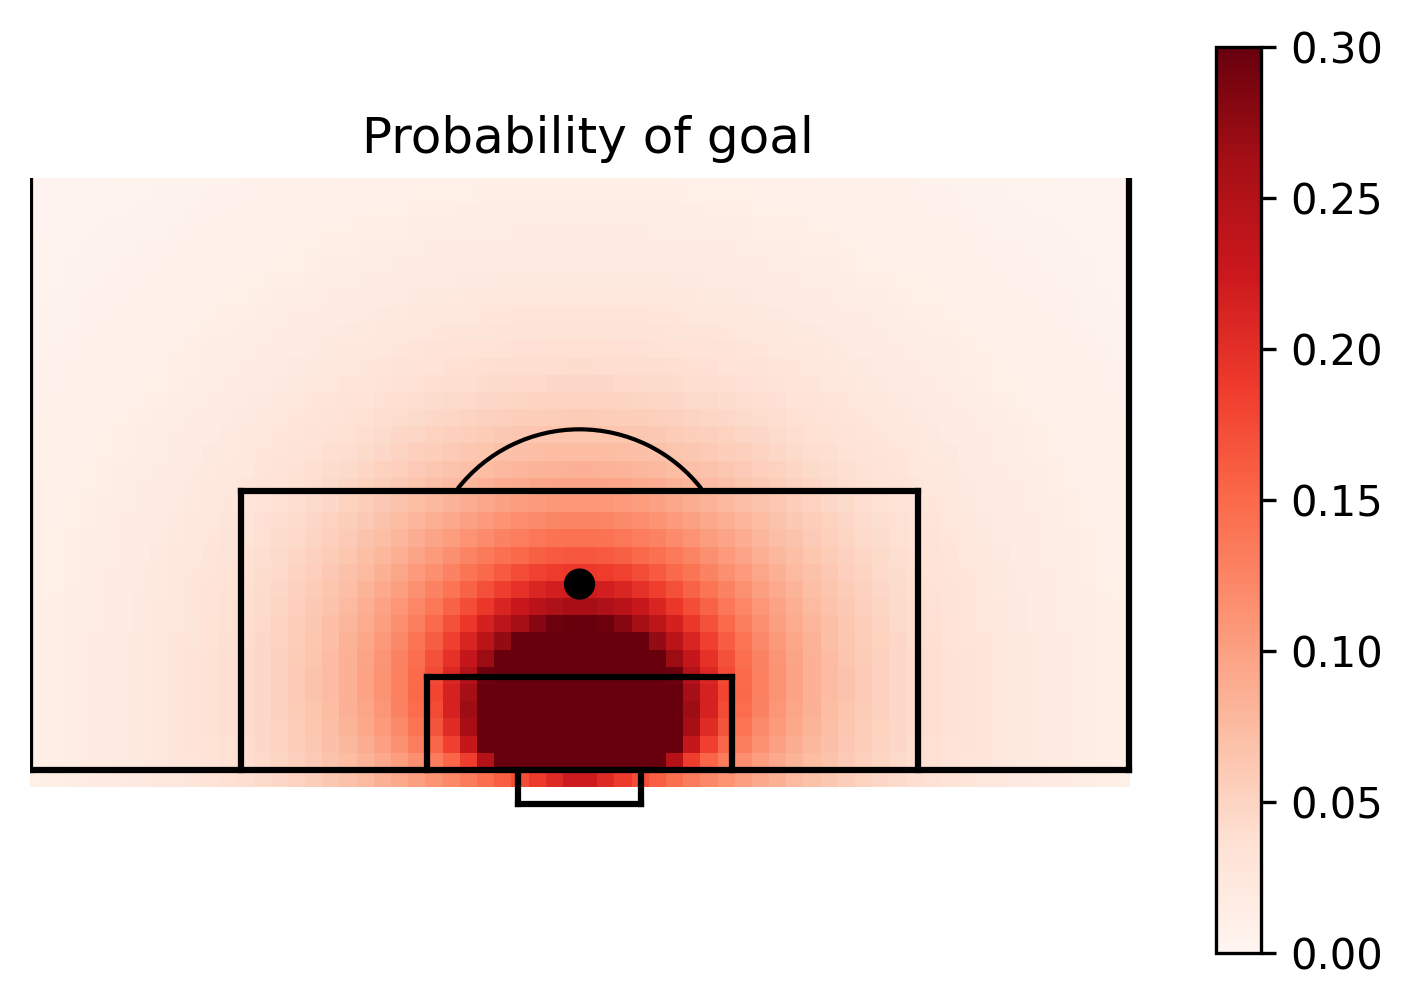
\includegraphics[scale=0.6]{images/xgplot2.png}   
    \caption{Histogram of xG values around the opposition's box.}
    \label{fig:xgz} 
\end{figure}

\begin{figure}[h]
    \centering
    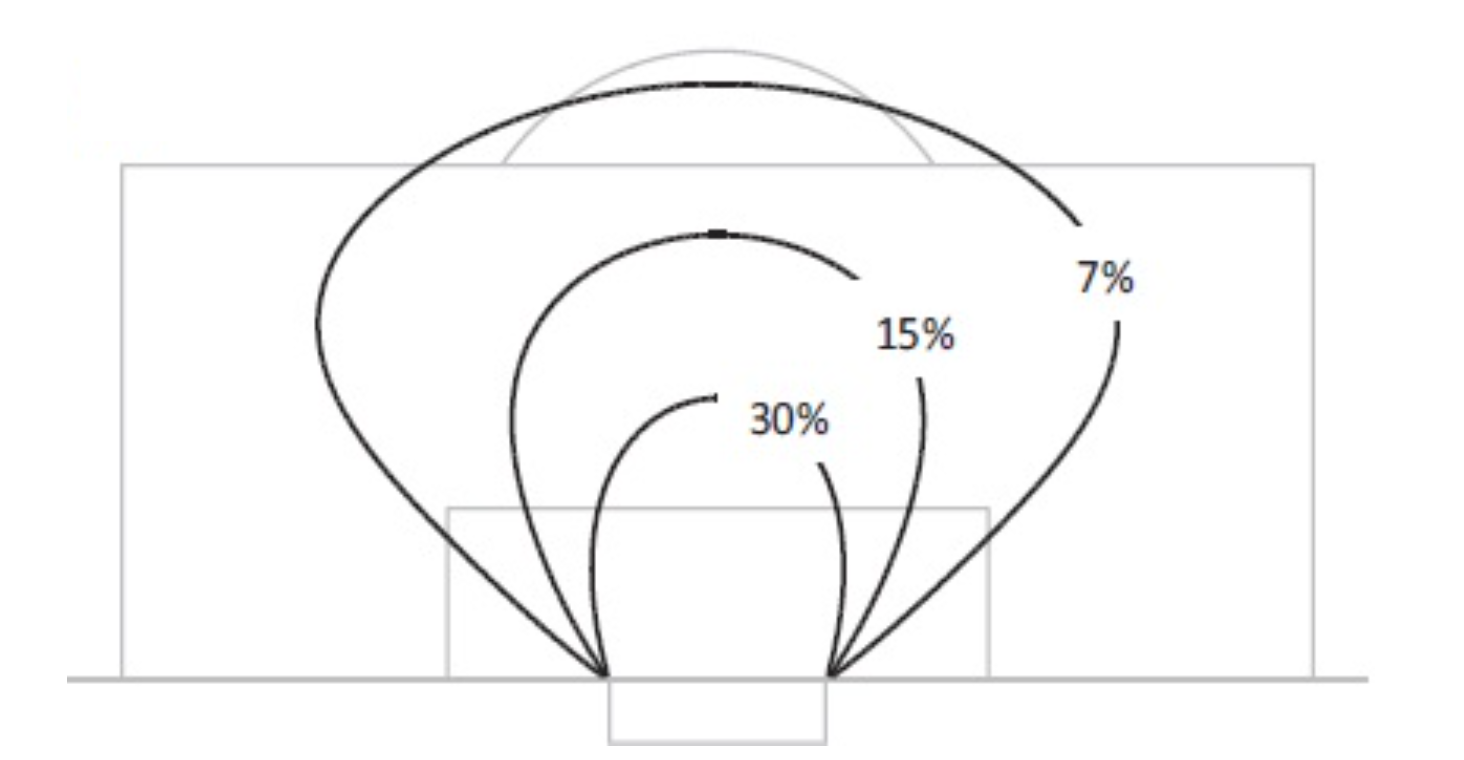
\includegraphics[scale=0.4]{images/sumpterxG.png}   
    \caption{Diagram showing xG 'rings', often used to give a rough, illustrative notion of xG. Used at clubs such as Hammarby Fotboll (reproduced from Sumpter's Soccermatics \cite{sump1}).}
    \label{fig:xgsum} 
\end{figure}

While many further refinements are possible, this model is more than satisfactory for our purposes of defining an \textit{average xG} for each state in our Markov models.

\section{Building a Possession Model in PRISM}

Before defining models in PRISM, we must first define our states. We begin with a simple set of location-based, ball-in-play states, based on Rudd's framework \cite{rudd1}. The opposition's half is divided into 7 zones each representing a state (\textbf{Fig. \ref{fig:zooones}}). The position of the ball in possession (i.e. which zone it is in) determines what state the system is in. Transitions occur when a player's action moves the ball from one zone to another (or into the same zone). In our initial model, we also define two absorbing states - \textit{loss of possession}\footnote{This occurs when a player action results in the opposition gaining control of the ball, or the ball going out of play.} and \textit{goal scored}, giving us a total of 9 states.

In our PRISM descriptions (included as appendices) we define a variable $s$ to represent our states. Therefore, we will refer to our 7 in-play states as ($s_0 ... s_6$). Our two absorbing states, $s_7$ and $s_8$, are explicitly labelled \texttt{possession\_lost} and \texttt{goal}.

\begin{figure}[h]
    \centering
    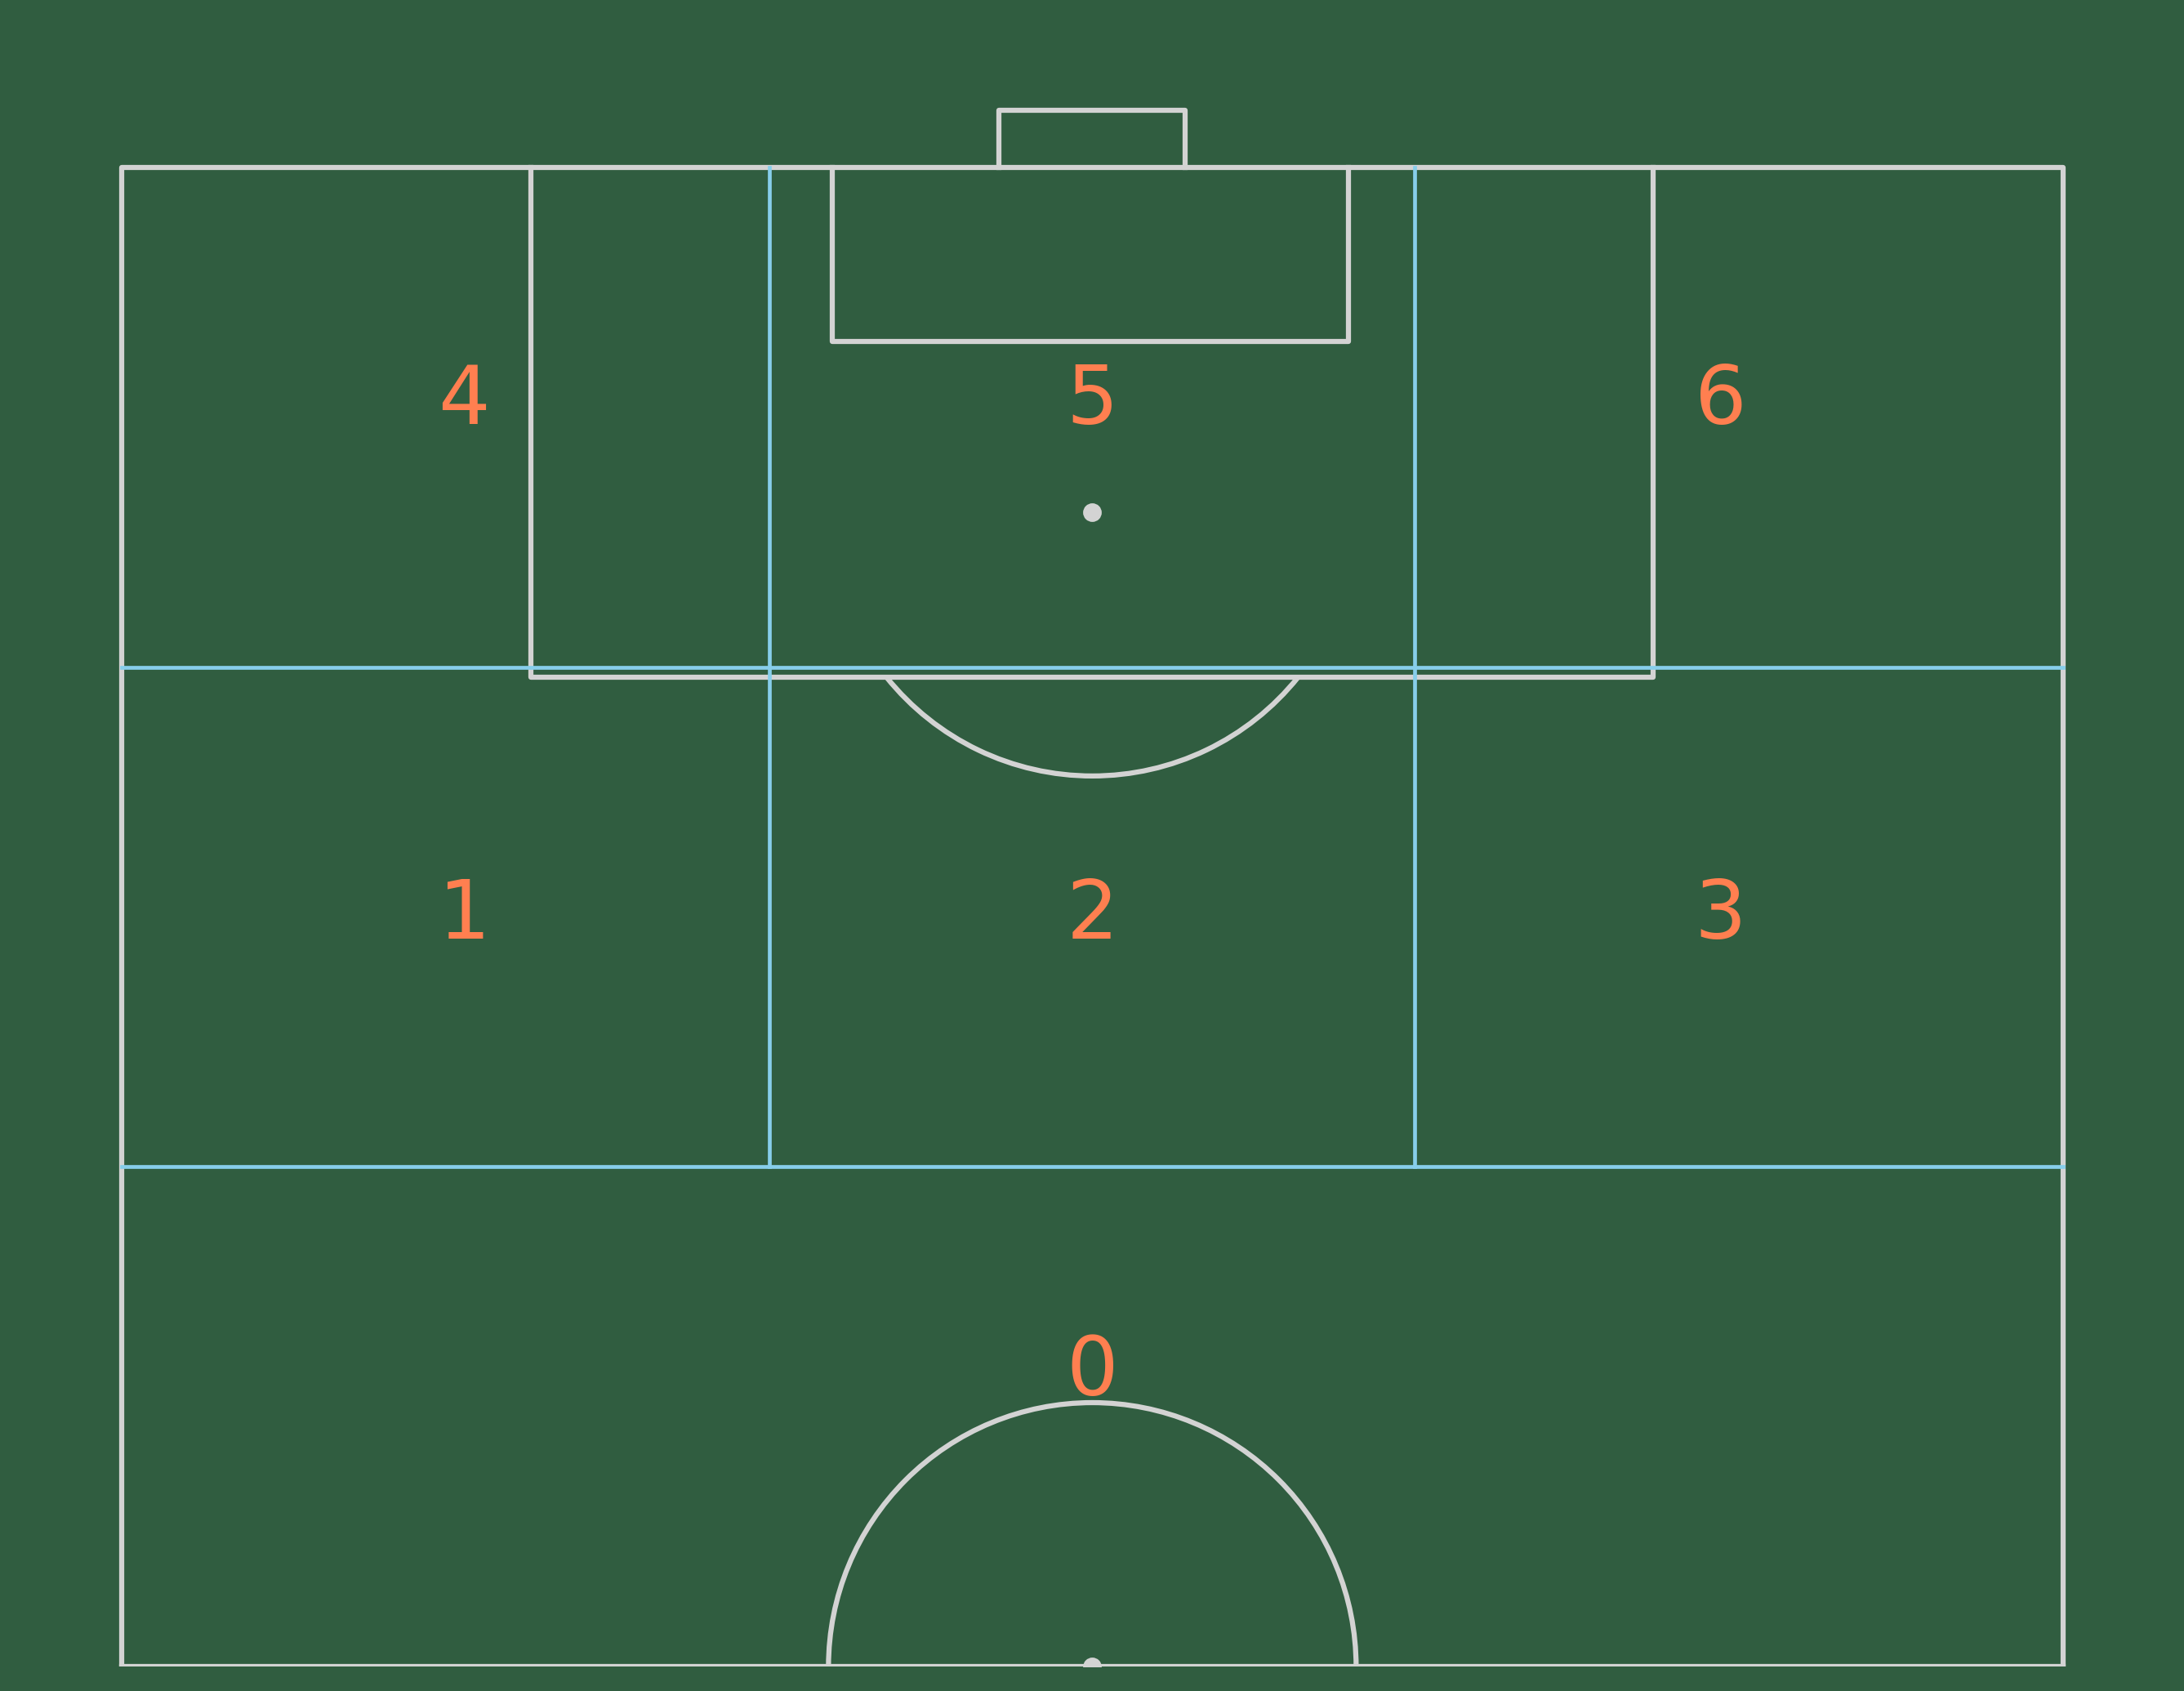
\includegraphics[scale=0.4]{images/states1.png}   
    \caption{Zones defined for the location-based states used in our early model. Zones of the pitch are drawn along similar lines to those of Rudd's framework \cite{rudd1}. Zones 1-6 make up what is commonly referred to as the `attacking third' in football. Note that the view of the pitch has been rotated $180^{\circ}$ with respect to previous visualisations.}
    \label{fig:zooones} 
\end{figure}

\subsection{Possession as a Discrete-time Markov Chain}

We know (from \cite{fac2}) that Markov decision processes will allow us to model non-deterministic (a player's chosen action) and probabilistic (the outcome of that action) behaviours and synthesise strategies using PRISM. However, we first construct a discrete-time Markov chain - a simpler representation - to see what insights, if any, we can gain about the data or football strategy.

We begin by calculating our probability distributions, by examining the start and end points of each player action. We use Python to iterate over a \textit{pandas} data frame of all qualifying\footnote{See the limitations listed at the beginning of this chapter for details.} events and populate a 9-by-9 matrix with a count of each transition. These counts are converted to probabilities to create a \textit{transition probability matrix} for use with our model.

\begin{figure}[h]
    \centering
    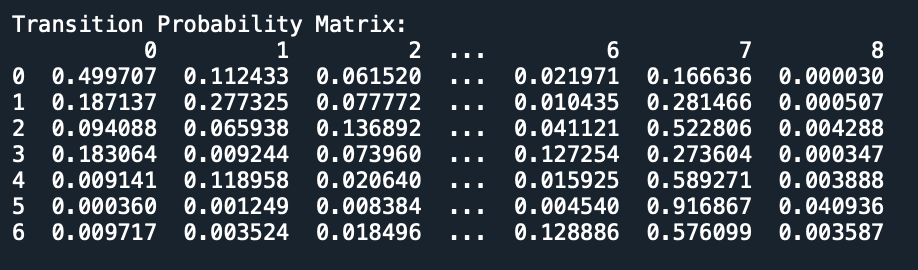
\includegraphics[scale=0.6]{images/probmat.png}   
    \caption{Console output showing the (truncated) transition probability matrix generated by the Python script. Outbound transitions from absorbing states (rows 7 and 8) have been omitted.}
    \label{fig:probmat} 
\end{figure}

We use simple string concatenation to populate a template DTMC specification in the PRISM modelling language with these transition probabilities, and write it to a \textit{.pm}\footnote{The PRISM model file extension.} file for use with the PRISM model checker. The source code to calculate probabilities and write the PRISM model file can be found in \texttt{/code/python/extract\_wyscout\_data.py}. The PRISM model file is written to \texttt{/code/prism/markovchain.pm}. The complete listing is available in the appendices (\textbf{Appendix \ref{lst:appendix2}}).

We can verify this model in PRISM and evaluate queries, such as "what is the probability that, eventually, a goal will be scored?" In PRISM's property specification language, this is:

\begin{center}
    \texttt{\textbf{P}=? [ \textbf{F} "goal" ]}
\end{center}

In terms of strategy generation, our DTMC does not offer a great deal of value. We would expect, based on our xG model, that the state with the highest probability of a goal would be $s_5$. PRISM confirms this by running a series of simulation taking states 0-6 as the initial state (\textbf{Fig. \ref{fig:sim1}}).

\begin{figure}[h]
    \centering
    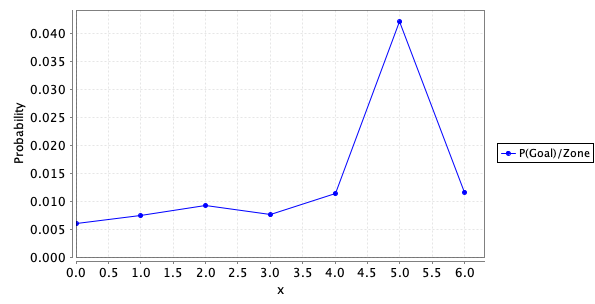
\includegraphics[scale=0.6]{images/probabilityofscoring.png}   
    \caption{PRISM-generated graph showing the probability of a goal being scored (eventually) in each state (x). The probability of a goal is at its greatest (approximately 4\%) in state 5.}
    \label{fig:sim1} 
\end{figure}

The rules of football allow the ball in play to be played anywhere within the pitch (with the exception of offside\footnote{A player is said to be offside when he or she receives a pass with fewer than two opposition players between said player and the goal line. Offside is not modelled here, but is touched upon in later sections.}. situations). In our current model, the most fruitful path will always be to pass the ball to $s_5$ and shoot. The best football strategy we can infer here is to kick the ball into the box, which is not revelatory to anyone familiar with the game.

\subsection{Possession as a Markov Decision Process}

In addition to the states defined for our DTMC, our MDP requires a set of \textit{actions} - that is, for a given state, multiple, labelled commands which may be executed. This allows the model's module to make non-deterministic choices - as a football player might in an attacking situation.

For each of our in-play states ($s_0 ... s_6$), we define six passing actions, labelled \texttt{pass\_a\_b}. These can be read as "pass from  $s_a$ to $s_b$". Each state also has a seventh action, \texttt{shoot\_a}, representing a shot on goal from $s_a$.

Once again, we make use of Python to extract the relevant probabilities from the data set. The process is similar to the generation of the DTMC, but there is an additional challenge in modelling the non-deterministic choice involved in each transition.

Specifically, in order to establish a reasonable probability distribution across each action, we must determine the action that was chosen by a player. The data can tell us whether or not a pass is successful, but in cases where it is not, we have no way of knowing what the intended destination was.

Our approach is to make the assumption that unsuccessful passes at least reached their intended zone, given that the zones defined are large, and a likely reason for failure is an interception by a marker - an opposition player who is trying to prevent a pass reaching its intended recipient. On this basis, we consider a failed pass from \texttt{a} that lands in a particular zone \texttt{b} as a \texttt{pass\_a\_b} action which resulted in loss of possession. 

We iterate over the events, extracting shots and passes in the opposition's half. A 2-dimensional array called \texttt{trans\_mat} is populated with a count of:

\begin{itemize}
    
    \item failed shots;
    \item failed passes;
    \item successful shots;
    \item successful passes.

\end{itemize}

A second, \texttt{decision\_mat}, is populated with a count of \textit{attempted} shots and passes. Through simple division, we can obtain the probabilities that each \textit{decision} is successful (a pass is completed or a goal is scored) or otherwise (possession is lost). Equipped with these probability distributions across actions, we can now insert them into a string - an MDP template - and write to a \textit{.pm} file.

The python script that extracts the probabilities and generates our MDP in the PRISM language can be found in the source code at \texttt{/code/python/extract\_wyscout\_data\_2.py}. The generated PRISM file can be found at \texttt{/code/prism/markovdecisionprocess.pm}. The full model listing is available in the appendices (\textbf{Appendix \ref{appendix3}}).

Before performing any further refinements, we perform a simple PRISM experiment, similar to the earlier one on the DTMC, for some very basic insights. We evaluate the query, \textit{"what is the \textit{maximum} probability (over all possible paths) that a goal will, eventually, be scored?"} In PRISM's property specification language: 

\begin{center}
    \texttt{\textbf{Pmax}=? [ \textbf{F} "goal" ]}
\end{center}

Our experiment checks this probability across all possible initial states. We see a graph (\textbf{Fig. \ref{fig:sim2}}) similar to the previous one, albeit with higher probabilities. This is because PRISM has determined the \textit{best} path, exploring all possible outcomes of non-determinism.

\begin{figure}[h]
    \centering
    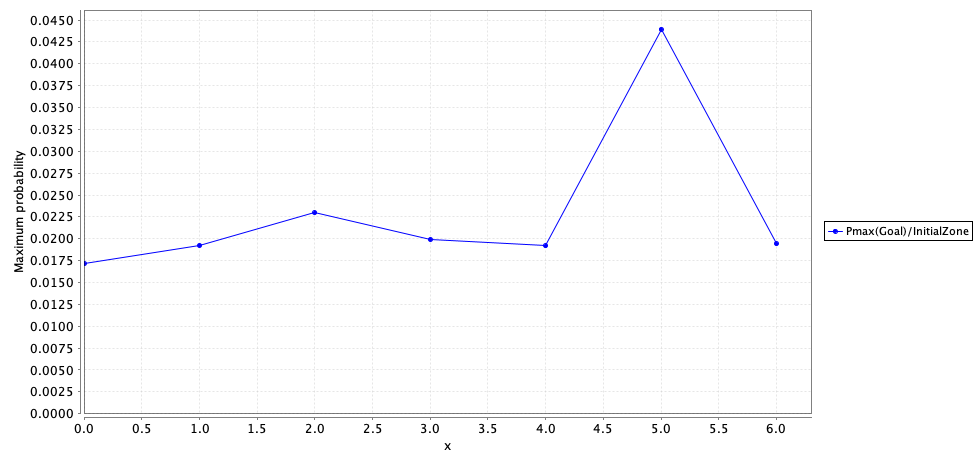
\includegraphics[scale=0.4]{images/prob_score2.png}   
    \caption{PRISM-generated graph showing the maximum probability of a goal being scored (eventually) in each state (x).}
    \label{fig:sim2} 
\end{figure}

\subsection{Further Refinements}

Given the fidelity of our data, more granularity could provide a more accurate and interesting model. For this reason, we revisit our location-based states. To provide deeper insight about where the ball is moving to and from, we divide the opposition's half up into smaller zones (\textbf{Fig. \ref{fig:zones2}}). We split the midfield zone, 0, into left and right midfield zones, now 0 and 1. Each of the existing zones 1-6 in the attacking third are quartered, giving us a total of 27 location-based states. 

\begin{figure}[h]
    \centering
    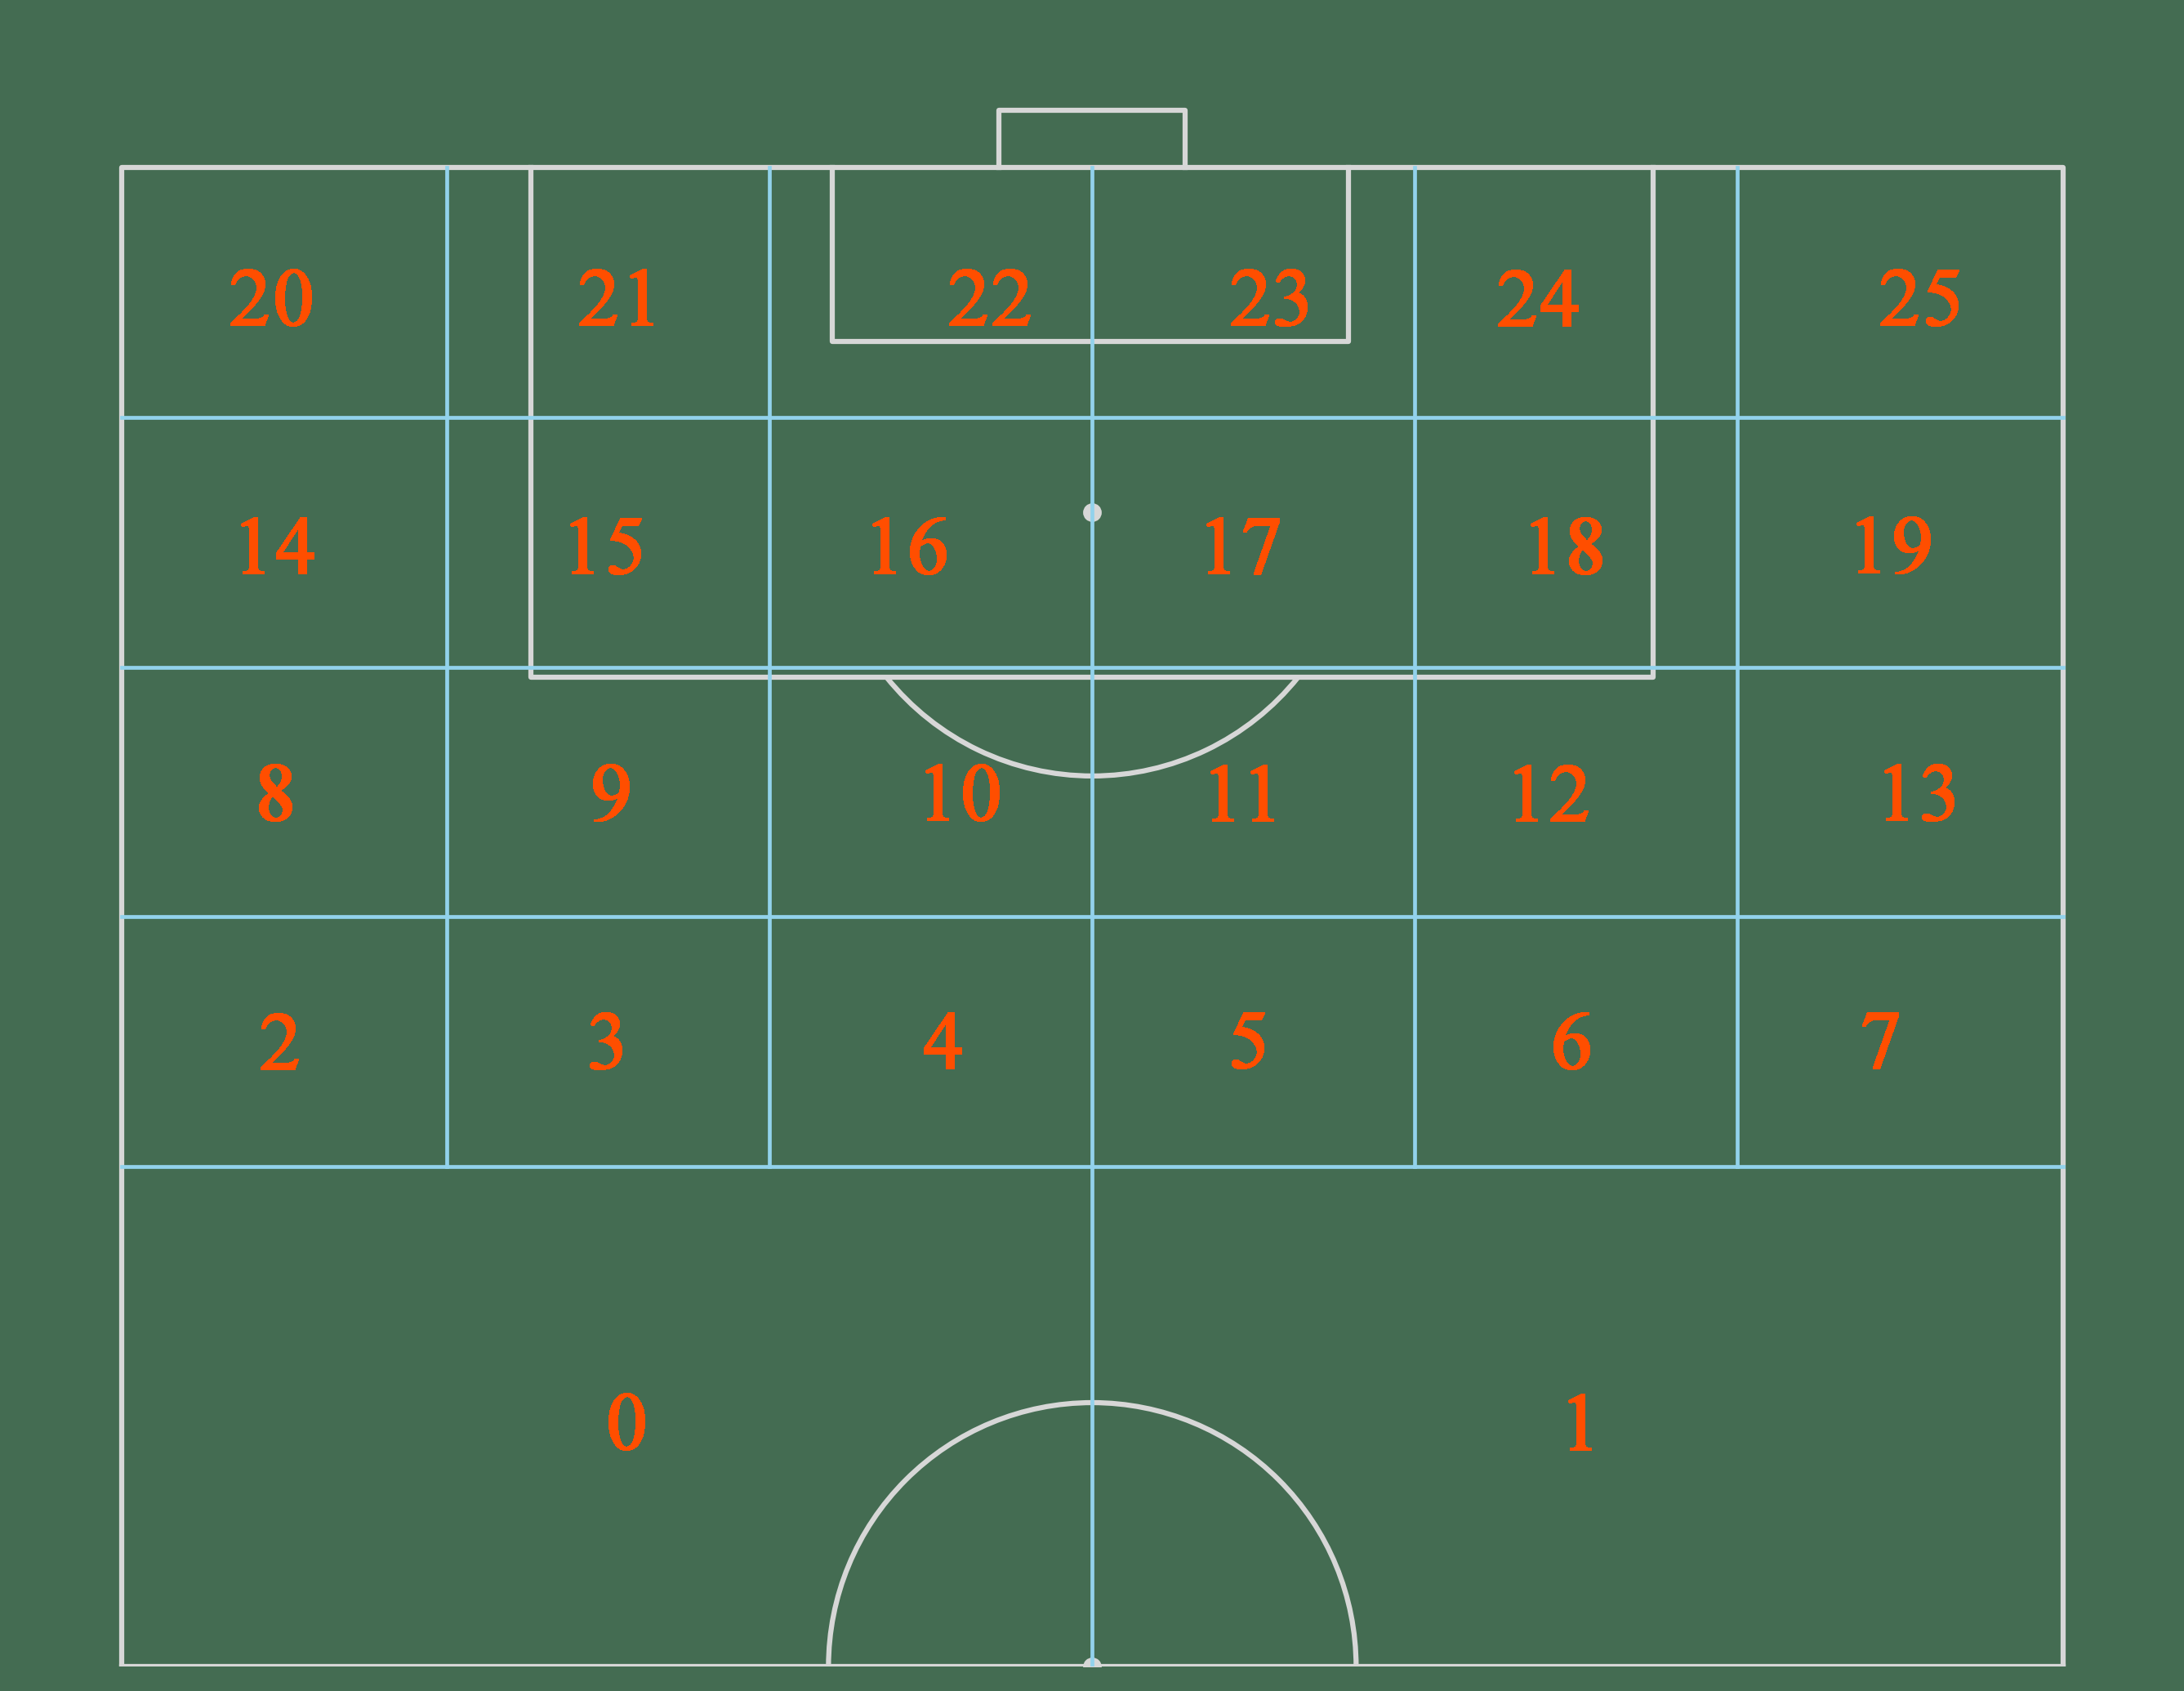
\includegraphics[scale=0.4]{images/zones2.png}   
    \caption{Our second iteration of the MDP divides the pitch into 26 zones, offering a more fine-grained representation of the ball moving around the pitch.}
    \label{fig:zones2} 
\end{figure}

We refactor our Python script to populate a new PRISM file based on the expanded state space. The model specification generated is valid and can be built in PRISM, but there are further refinements to be made.

There are a number of actions which represent decisions that are never taken in our data. These actions are:

\begin{itemize}
    \item \texttt{pass\_22\_2}
    \item \texttt{pass\_22\_6}
    \item \texttt{pass\_22\_11}
    \item \texttt{pass\_22\_12}
    \item \texttt{pass\_23\_0}
    \item \texttt{pass\_23\_5}
\end{itemize}

As we have no sample outcomes, we have no way to determine a probability distribution for these actions. Rather than leave these actions in the model with deterministic outcome of \texttt{possession\_lost} (which may be an equally valid approach), we choose to remove them.

Additionally, we augment the probabilities that shot actions in the attacking third will transition to the goal state, using our modelled xG. We calculate an average xG across all of the values generated from our model in section \textbf{\ref{xgsection}} which fall within our pitch zones. These are shown (to four decimal places) in \textbf{Fig. \ref{fig:zonesxgd}}.

The Python script to generate this final PRISM model can be found in the source code via the path \texttt{/code/python/extract\_wyscount\_data\_3.py}. The generated PRISM model is written to \texttt{/code/prism/markovdecisionprocess2.pm}. The full listing of the MDP at this stage is included in the appendices (\textbf{Appendix \ref{appendix4}}).

\begin{figure}[h]
    \centering
    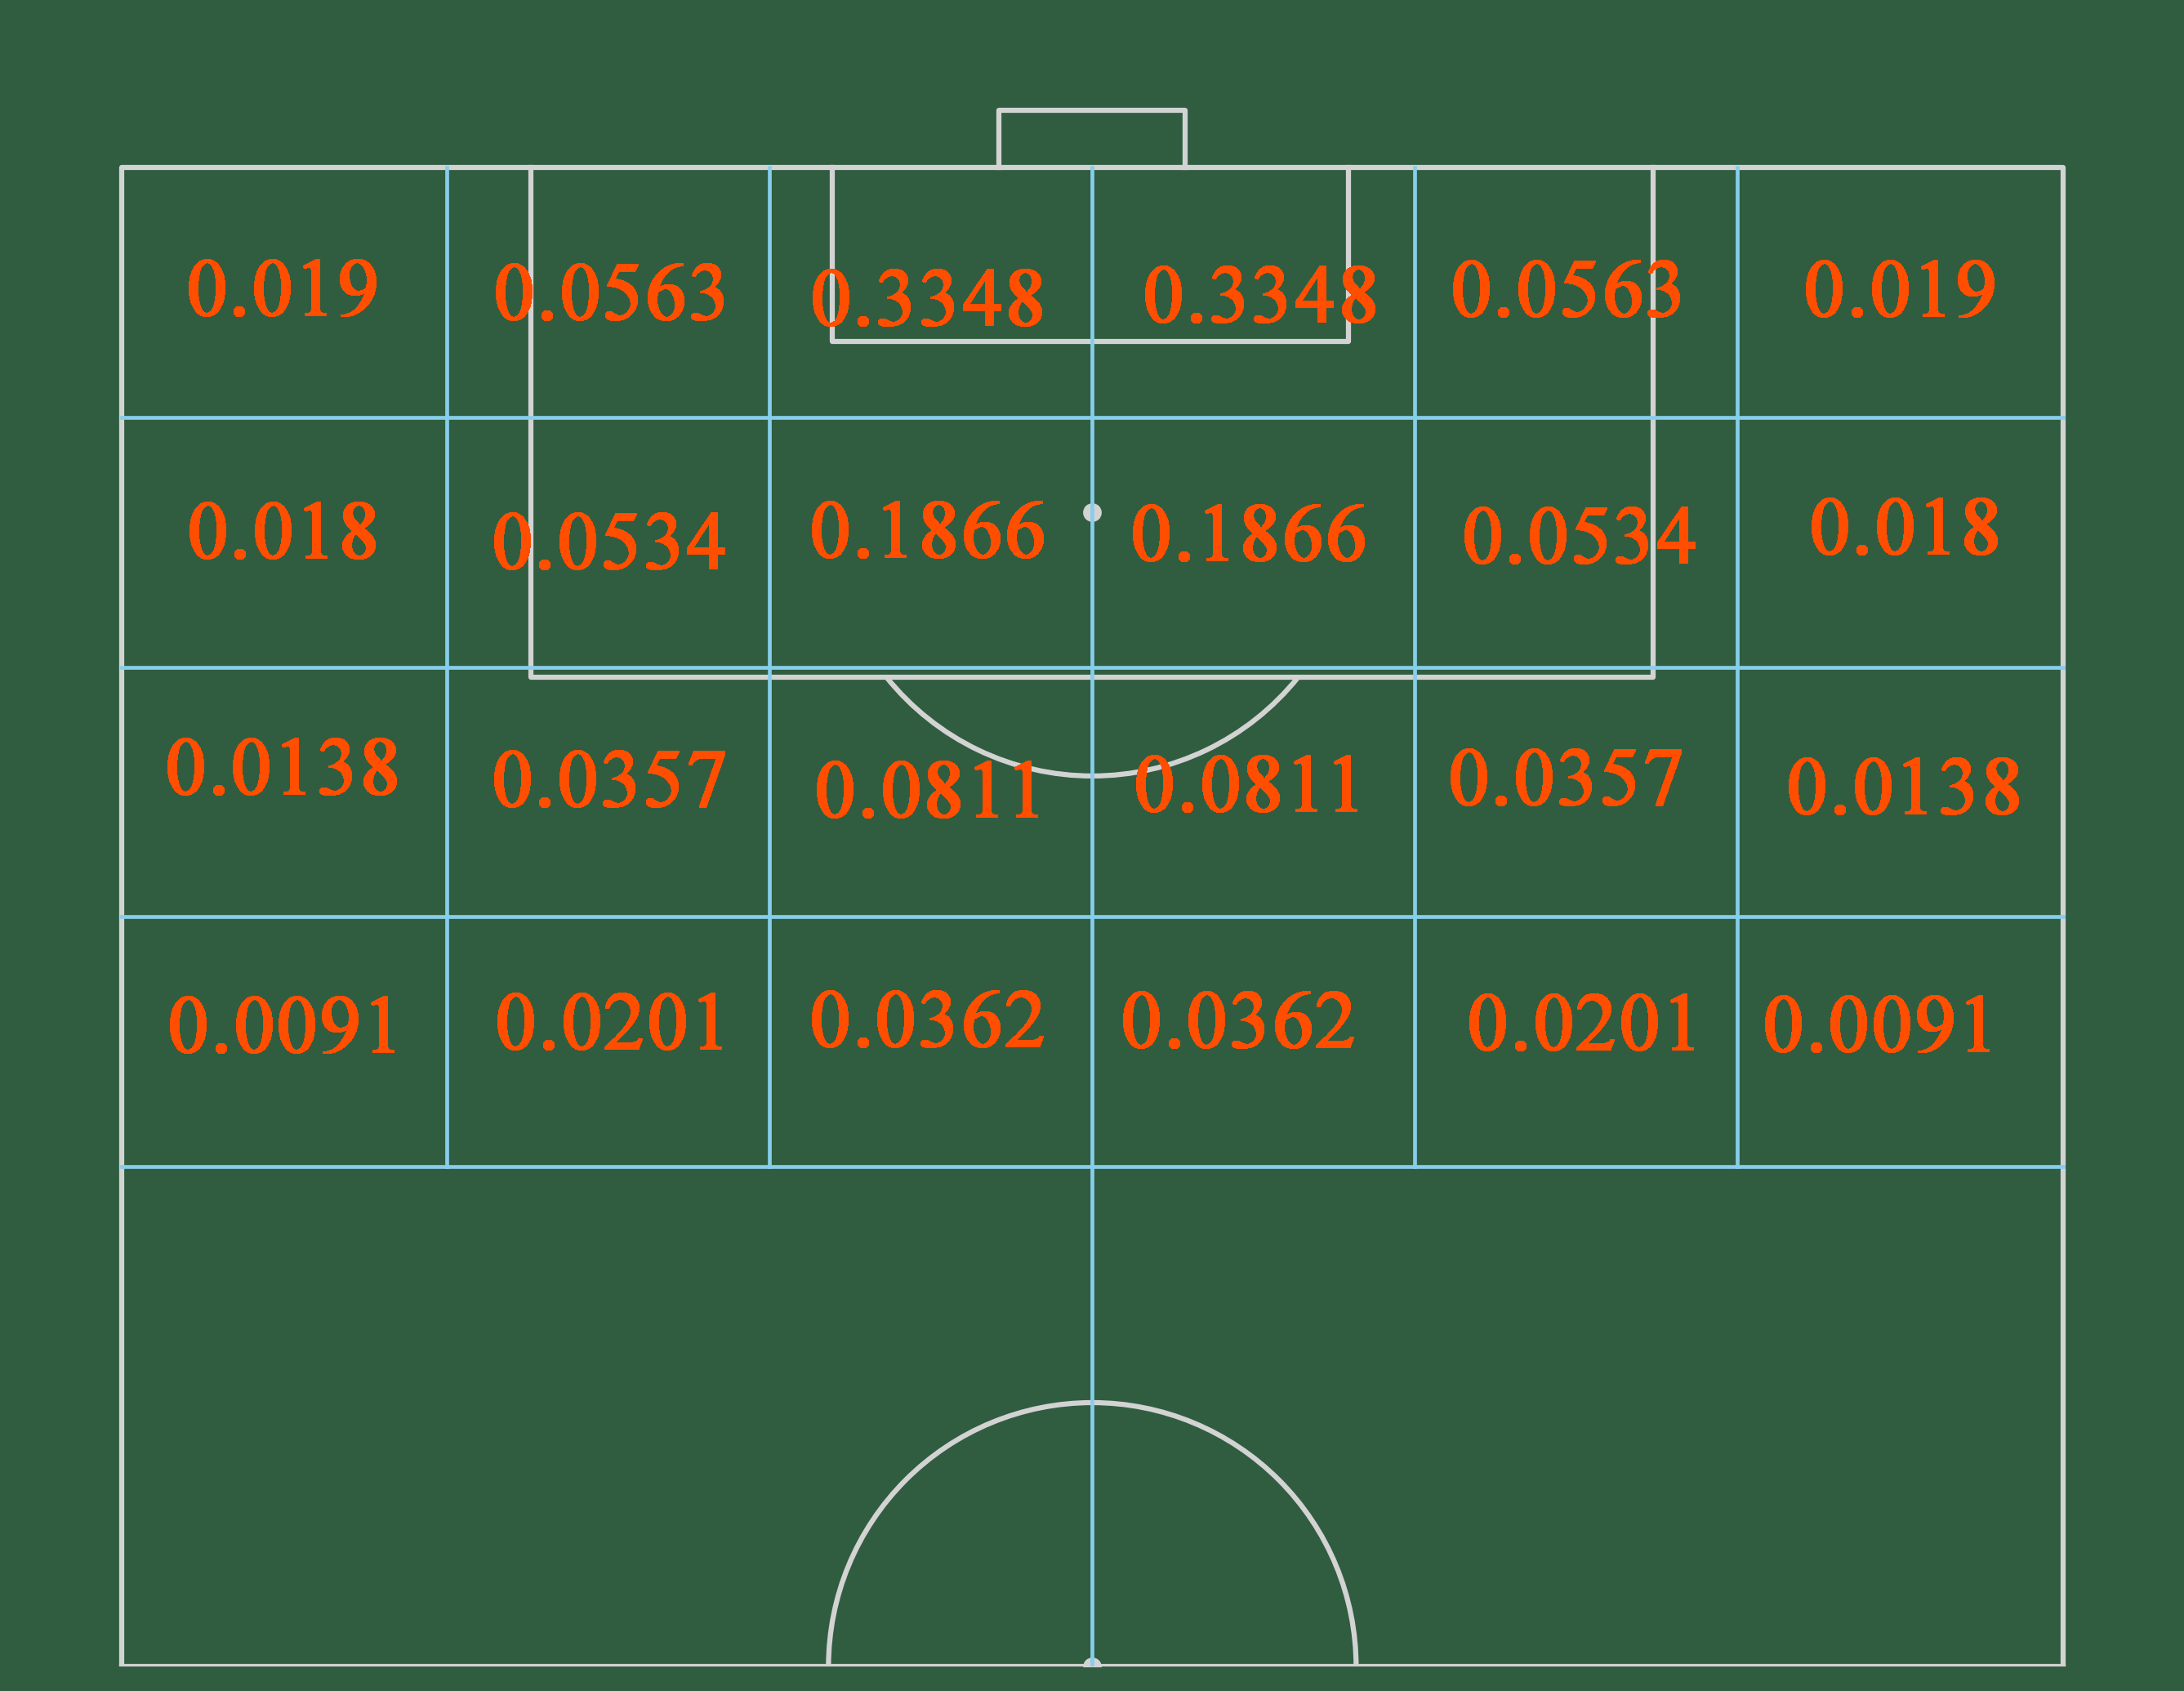
\includegraphics[scale=0.1]{images/xoneswxg.png}   
    \caption{Approximate (to four decimal places) average xG values as per our earlier model, overlaid on their respective zones.}
    \label{fig:zonesxgd} 
\end{figure}

%==================================================================================================================================
\chapter{Strategy Synthesis}

One of PRISM's most powerful features is its capacity to determine an optimal path through a stochastic, non-deterministic system (represented as an MDP) that satisfies a particular property or properties. This is achieved by the generation of an \textit{optimal adversary}.

\section{PRISM Adversaries}

Adversaries in PRISM \cite{prsmlang} produce an optimal set of action choices for each state in the MDP. Since only one choice is presented per state, the non-determinism of the model is obviated and the adversarial choices are returned as a DTMC. 

Our goal is to generate strategies with "maximal scoring potential" and we therefore want to generate an adversary based upon the property:

\begin{center}
    \texttt{\textbf{Pmax}=? [ \textbf{F} "goal" ]}
\end{center}

We can generate such an adversary by passing the model and the property to prism in the command line, with the \texttt{-exportadv} flag. To better understand adversaries, we first generate a simple strategy for our initial MDP (\textbf{Appendix \ref{appendix3}}). The resultant adversarial choices are tabulated in \textbf{Table \ref{tab:adv-mdp1}}. 

\begin{table}[h]
\centering
\caption{PRISM generated adversary for simple MDP (\textbf{Appendix \ref{appendix3}}). In this model, $s_7$ is \texttt{possession\_lost} and $s_8$ is \texttt{goal}.}
\rowcolors{2}{}{gray!10}
\begin{tabular}{llll}
\textbf{State} & \textbf{State'} & \textbf{P}         & \textbf{Action}     \\
0     & 2      & 0.746688  & \texttt{pass\_0\_2} \\
0     & 7      & 0.253312  & \texttt{pass\_0\_2} \\
1     & 5      & 0.437603  & \texttt{pass\_1\_5} \\
1     & 7      & 0.562397  & \texttt{pass\_1\_5} \\
2     & 5      & 0.522698  & \texttt{pass\_2\_5} \\
2     & 7      & 0.477302  & \texttt{pass\_2\_5} \\
3     & 5      & 0.453146  & \texttt{pass\_3\_5} \\
3     & 7      & 0.546854  & \texttt{pass\_3\_5} \\
4     & 5      & 0.436356  & \texttt{pass\_4\_5} \\
4     & 7      & 0.563644  & \texttt{pass\_4\_5} \\
5     & 7      & 0.956052  & \texttt{shoot\_5}   \\
5     & 8      & 0.0439475 & \texttt{shoot\_5}   \\
6     & 5      & 0.441909  & \texttt{pass\_6\_5} \\
6     & 7      & 0.558091  & \texttt{pass\_6\_5}
\end{tabular}
\label{tab:adv-mdp1}
\end{table}

Although straightforward, we are able to extract a strategy from these choices which, based on our model, yields the best chance of scoring:

\clearpage
\begin{lstlisting}[language=Haskell, numbers=left, caption=Strategy with optimal probability of goal generated by PRISM from our initial MDP.] 
if s == 5 :
    shoot;
if s == 0 :
    pass to 2;
else:
    pass to 5;
\end{lstlisting}

We will discuss what this means in footballing terms in section \ref{sec:results}.

We repeat this process for the more complex MDP (\textbf{Appendix \ref{appendix4}}). The adversarial choices are presented in \textbf{Table \ref{tab:adv-mdp2}}. 

\begin{table}[h]
\centering
\caption{PRISM generated adversary for complex MDP (\textbf{Appendix \ref{appendix4}}). In this model, $s_{27}$ is \texttt{goal}. Due to space limitations, we have omitted the transitions into $s_{26}$ or  \texttt{possession\_lost}. The complete table has an accompanying row for each one presented below, with a probability of $(1-P)$ that the action will result in loss of possession.}
\label{tab:adv-mdp2}
\rowcolors{2}{}{gray!10}
\begin{tabular}{llll}
\textbf{State} & \textbf{State'} & \textbf{P}         & \textbf{Action}     \\
0  & 5  & 0.790914 & \texttt{pass\_0\_5}   \\
%0  & 26 & 0.209086 & \texttt{pass\_0\_5}  \\
1  & 5  & 0.774676 & \texttt{pass\_1\_5}   \\
%1  & 26 & 0.225324 & \texttt{pass\_1\_5}   \\
2  & 4  & 0.859556 & \texttt{pass\_2\_4}   \\
%2  & 26 & 0.140444 & \texttt{pass\_2\_4}   \\
3  & 5  & 0.887842 & \texttt{pass\_3\_5}   \\
%3  & 26 & 0.112158 & \texttt{pass\_3\_5}  \\
4  & 22 & 0.519481 & \texttt{pass\_4\_22}  \\
%4  & 26 & 0.480519 & \texttt{pass\_4\_22}  \\
5  & 22 & 0.527778 & \texttt{pass\_5\_22}  \\
%5  & 26 & 0.472222 & \texttt{pass\_5\_22}  \\
6  & 4  & 0.871442 & \texttt{pass\_6\_4}   \\
%6  & 26 & 0.128558 & \texttt{pass\_6\_4}   \\
7  & 5  & 0.862836 & \texttt{pass\_7\_5}   \\
%7  & 26 & 0.137164 & \texttt{pass\_7\_5}   \\
8  & 4  & 0.879717 & \texttt{pass\_8\_4}   \\
%8  & 26 & 0.120283 & \texttt{pass\_8\_4}   \\
9  & 4  & 0.88456  & \texttt{pass\_9\_4}   \\
%9  & 26 & 0.11544  & \texttt{pass\_9\_4}   \\
10 & 22 & 0.493976 & \texttt{pass\_10\_22} \\
%10 & 26 & 0.506024 & \texttt{pass\_10\_22} \\
11 & 23 & 0.5      & \texttt{pass\_11\_23} \\
%11 & 26 & 0.5      & \texttt{pass\_11\_23} \\
12 & 5  & 0.882353 & \texttt{pass\_12\_5}  \\
%12 & 26 & 0.117647 & \texttt{pass\_12\_5}  \\
13 & 22 & 0.478659 & \texttt{pass\_13\_22} \\
%13 & 26 & 0.521341 & \texttt{pass\_13\_22} \\
14 & 23 & 0.453005 & \texttt{pass\_14\_23} \\
%14 & 26 & 0.546995 & \texttt{pass\_14\_23} \\
15 & 23 & 0.527778 & \texttt{pass\_15\_23} \\
%15 & 26 & 0.472222 & \texttt{pass\_15\_23} \\
16 & 23 & 0.603774 & \texttt{pass\_16\_23} \\
%16 & 26 & 0.396226 & \texttt{pass\_16\_23} \\
17 & 22 & 0.596774 & \texttt{pass\_17\_22} \\
%17 & 26 & 0.403226 & \texttt{pass\_17\_22} \\
18 & 22 & 0.5      & \texttt{pass\_18\_22} \\
%18 & 26 & 0.5      & \texttt{pass\_18\_22} \\
19 & 22 & 0.447214 & \texttt{pass\_19\_22} \\
%19 & 26 & 0.552786 & \texttt{pass\_19\_22} \\
20 & 23 & 0.479058 & \texttt{pass\_20\_23} \\
%20 & 26 & 0.520942 & \texttt{pass\_20\_23} \\
21 & 23 & 0.476684 & \texttt{pass\_21\_23} \\
%21 & 26 & 0.523316 & \texttt{pass\_21\_23} \\
22 & 26 & 0.665231 & \texttt{shoot\_22}    \\
%22 & 27 & 0.334769 & \texttt{shoot\_22}    \\
23 & 26 & 0.665231 & \texttt{shoot\_23}    \\
%23 & 27 & 0.334769 & \texttt{shoot\_23}    \\
24 & 22 & 0.466055 & \texttt{pass\_24\_22} \\
%24 & 26 & 0.533945 & \texttt{pass\_24\_22} \\
25 & 22 & 0.497642 & \texttt{pass\_25\_22} \\
%25 & 26 & 0.502358 & \texttt{pass\_25\_22}
\end{tabular}
\end{table}

We can extract a more interesting strategy from these results, described in \textbf{Listing \ref{lst:code12}}. The footballing implications of this strategy will again be discussed in the next section.

\clearpage
\begin{lstlisting}[language=Haskell, numbers=left, caption=Strategy with optimal probability of goal generated by PRISM from our refined MDP.] 
if s == (22 | 23) :
    shoot;
if s == (4 | 5 | 10 | 13 | 17 | 18 | 19 | 24 | 25) :
    pass to 22;
if s == (11 | 14 | 15 | 16 | 20 | 21) :
    pass to 23;
if s == (0 | 1 | 3 | 7 | 12 ) :
    pass to 5;
else:
    pass to 4
\end{lstlisting}\label{lst:code12}

\section{Results}\label{sec:results}

We now present a series of simple visualisations based on the adversaries generated by PRISM, which hopefully explain the strategic insights that we have gained from model checking. 

\subsection{Simple MDP - Play Through the Middle}

We first examine a strategy based on the adversary generated for the simple MDP in \textbf{Appendix \ref{appendix3}}. 

\begin{figure}[h]
    \centering
    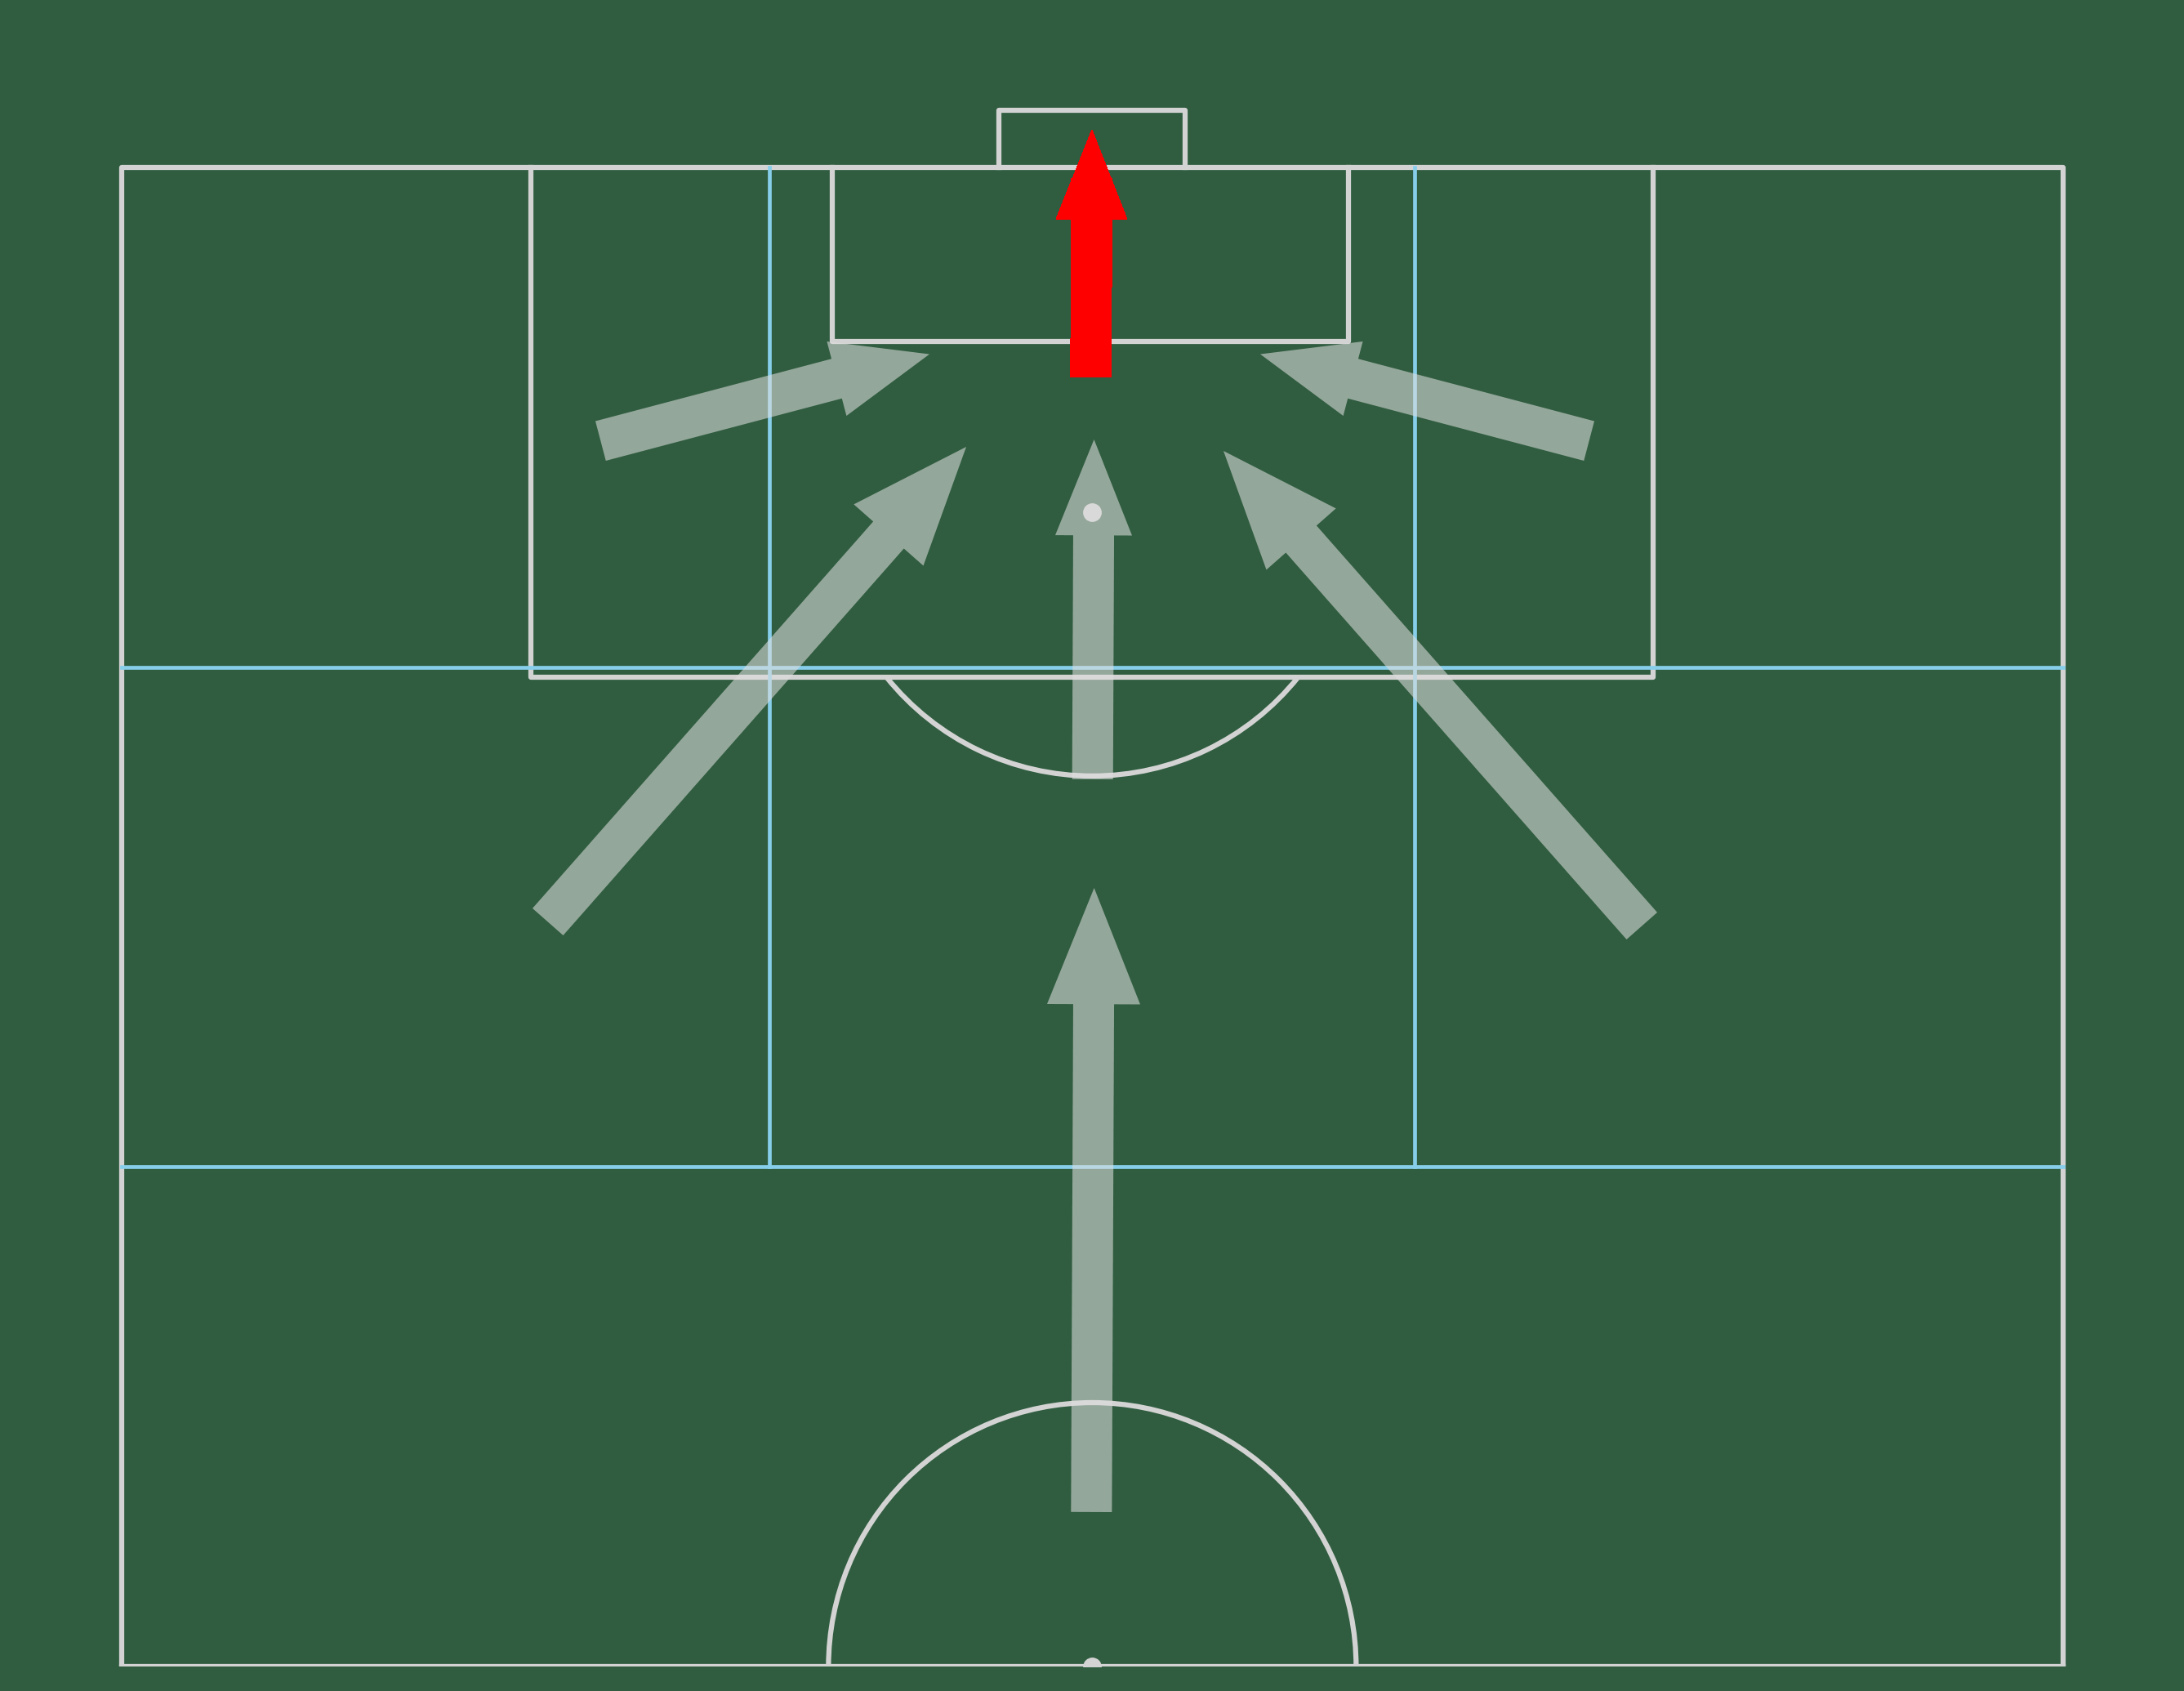
\includegraphics[scale=0.1]{images/bigzonestrat.png}   
    \caption{Diagram of optimal passes from each zone, as calculated by PRISM for our first MDP.}
    \label{fig:bigzonesstrat} 
\end{figure}

The graphic in \textbf{Fig. \ref{fig:bigzonesstrat}} represents the adversary's actions with arrows - the grey arrows are passes, and the red arrow is a shot. At first glance, it appears that the strategy is simply to move the ball into the middle of the box (\textit{Zone 5}) and shoot. However, based on the model provided, PRISM also advocates that the ball is played through the middle of the pitch from midfield, as opposed to the wings\footnote{The 'wings' are the outside channels of the pitch, closer to the touchlines.}.

Despite being a very simple model, our MDP is able to provide a valid strategy for build-up play when entering the attacking third.

\subsection{Refined MDP - Build-up Play}

Next, we examine strategies generated based on the second MDP (\textbf{Appendix \ref{appendix4}}). We have broken the visualisations for the more complex strategy into several panels based on phases of play. The first depicts optimal actions taken in the midfield and early in the attacking third.

\begin{figure}[h]
    \centering
    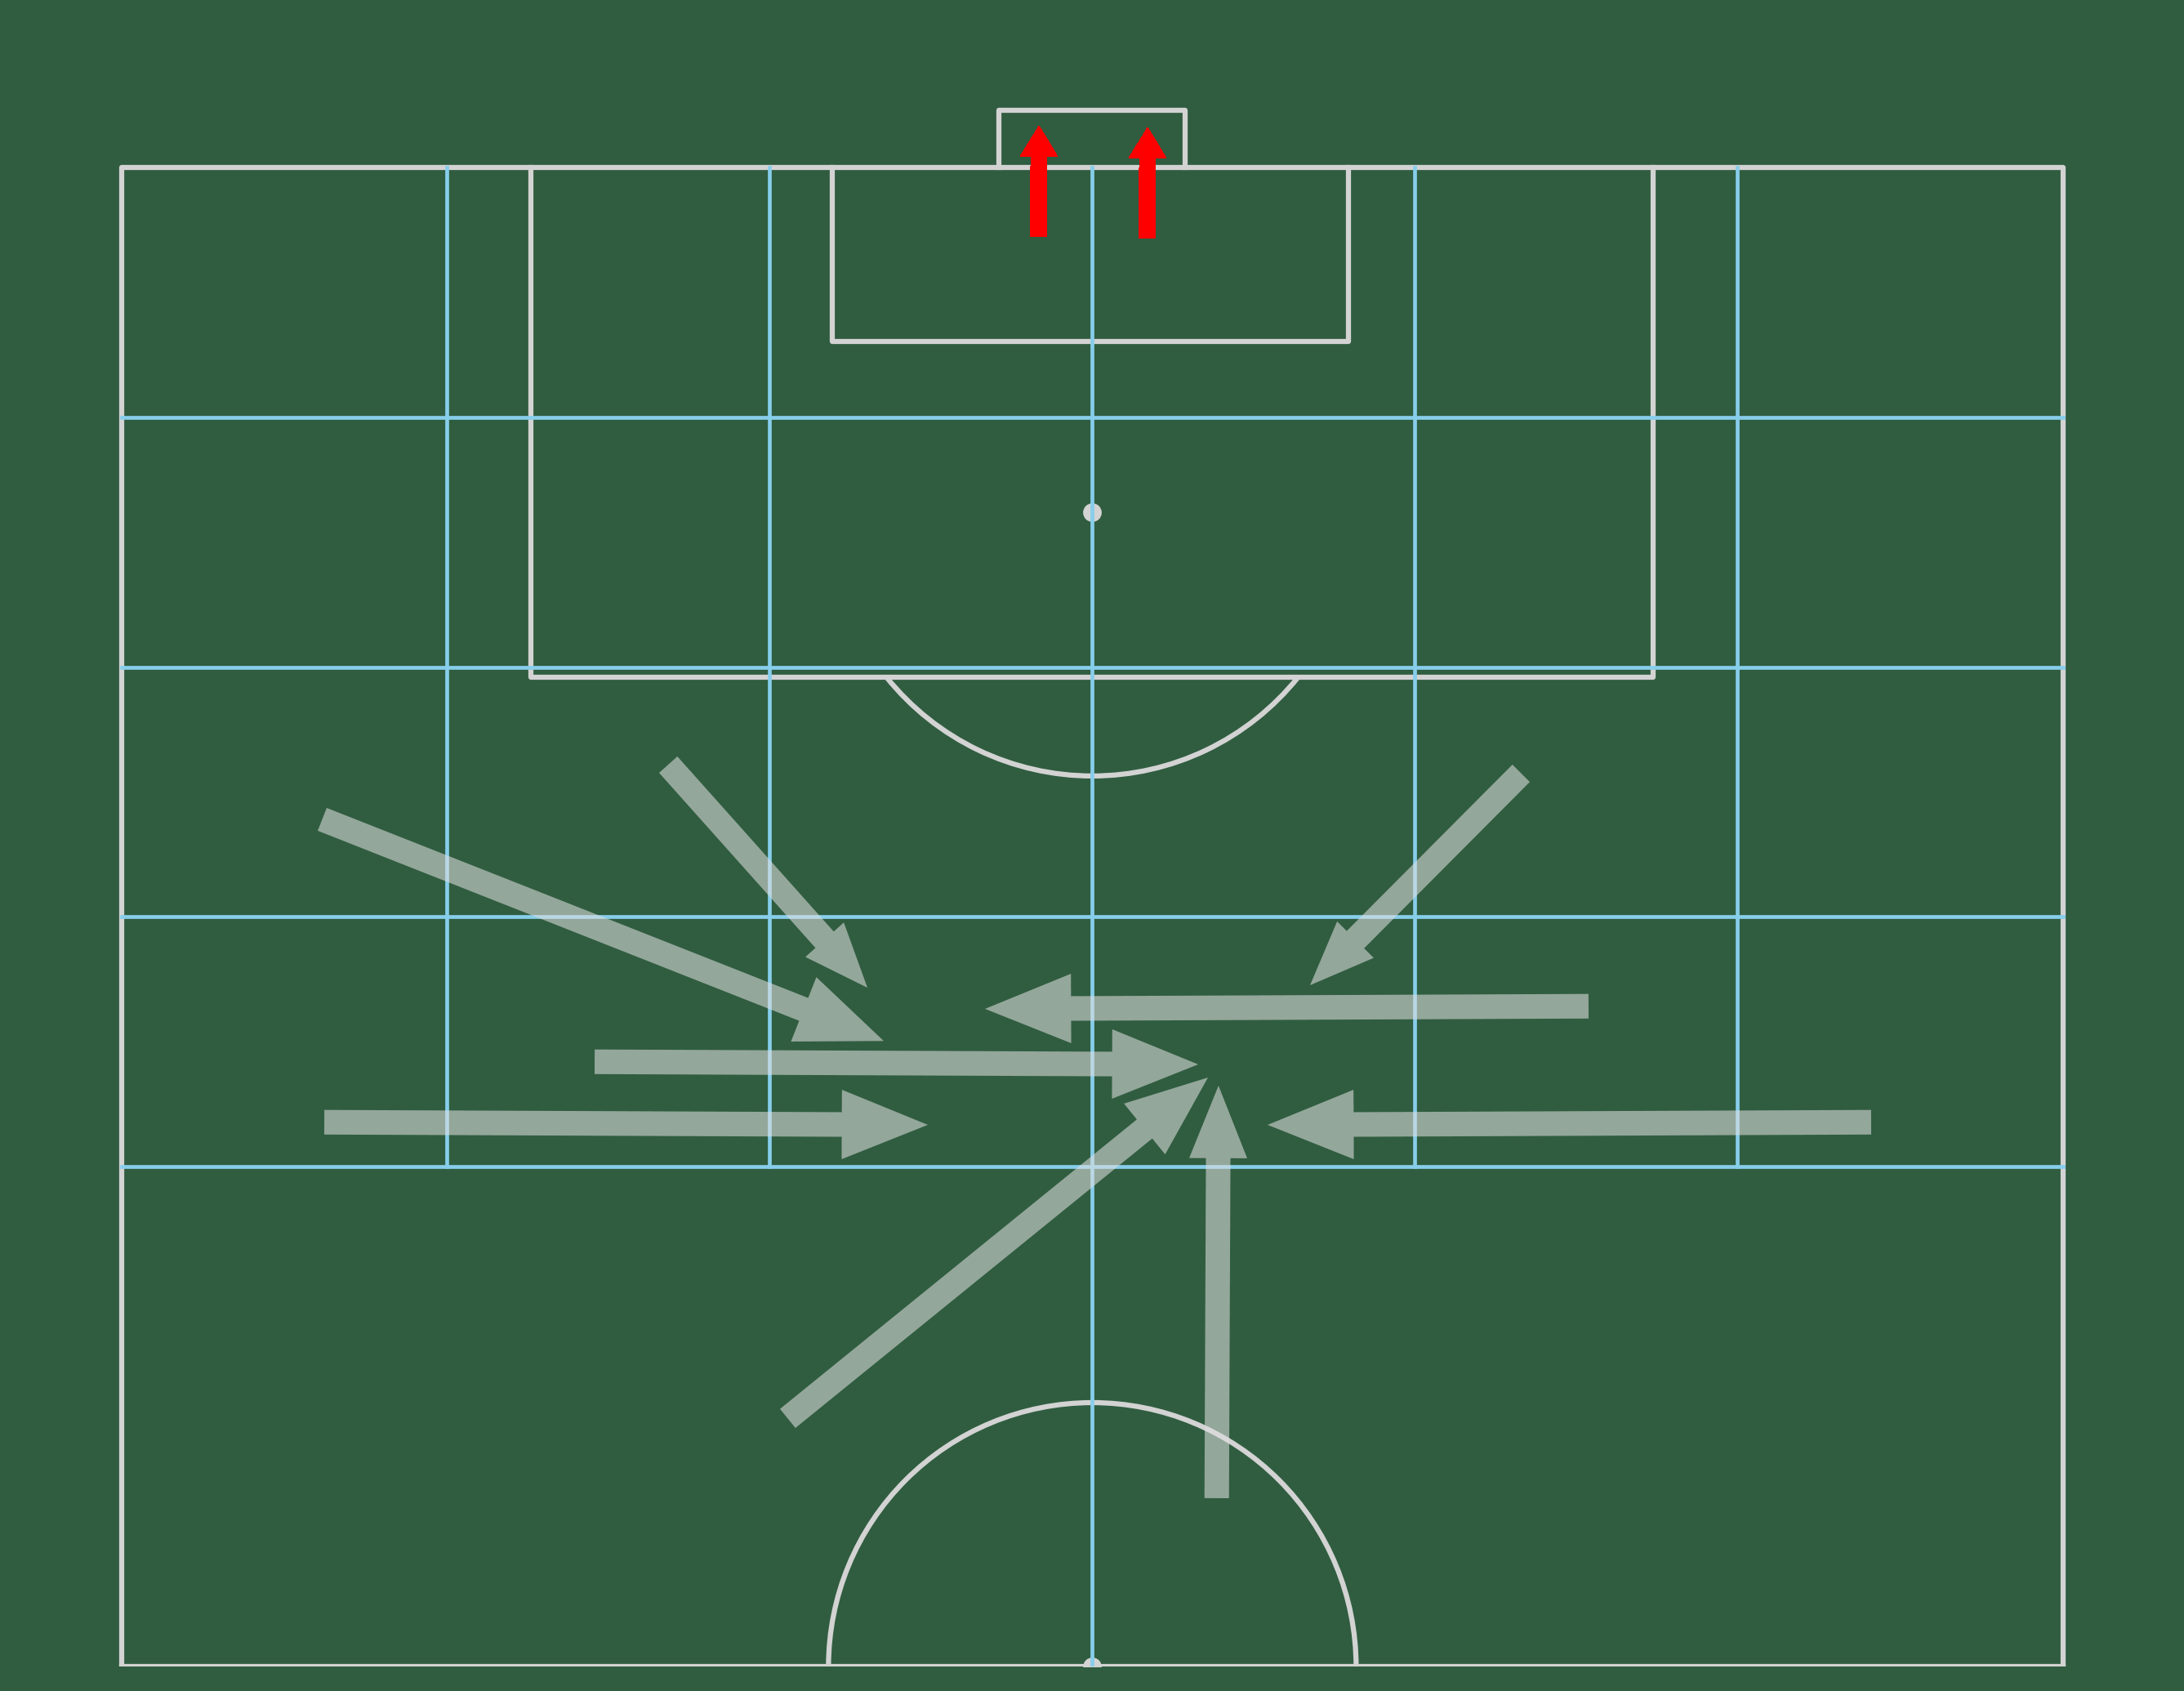
\includegraphics[scale=0.1]{images/buildupplay.png}   
    \caption{Diagram of optimal passes in build up play, from midfield and some less-advanced zones in the attacking third.}
    \label{fig:weezonebup} 
\end{figure}

The diagram (\textbf{Fig. \ref{fig:weezonebup}}) clearly shows a preference for moving the ball into central areas. The strategy dictates that the ball is moved from midfield into the right-of-centre zone, perhaps indicating a prevalence of right-footed midfielders in our data set. 

Perhaps most interestingly, the optimal strategy (based on the model) at the corners of the box (either side of the 'D') is to play the ball back towards midfield, rather than mount a direct attack on goal.

\subsection{Refined MDP - Early Crosses and Through Balls}

\textbf{Fig. \ref{fig:weezoneearl}} shows an optimal strategy for advancing the ball into the box early in an attacking move.

\begin{figure}[h]
    \centering
    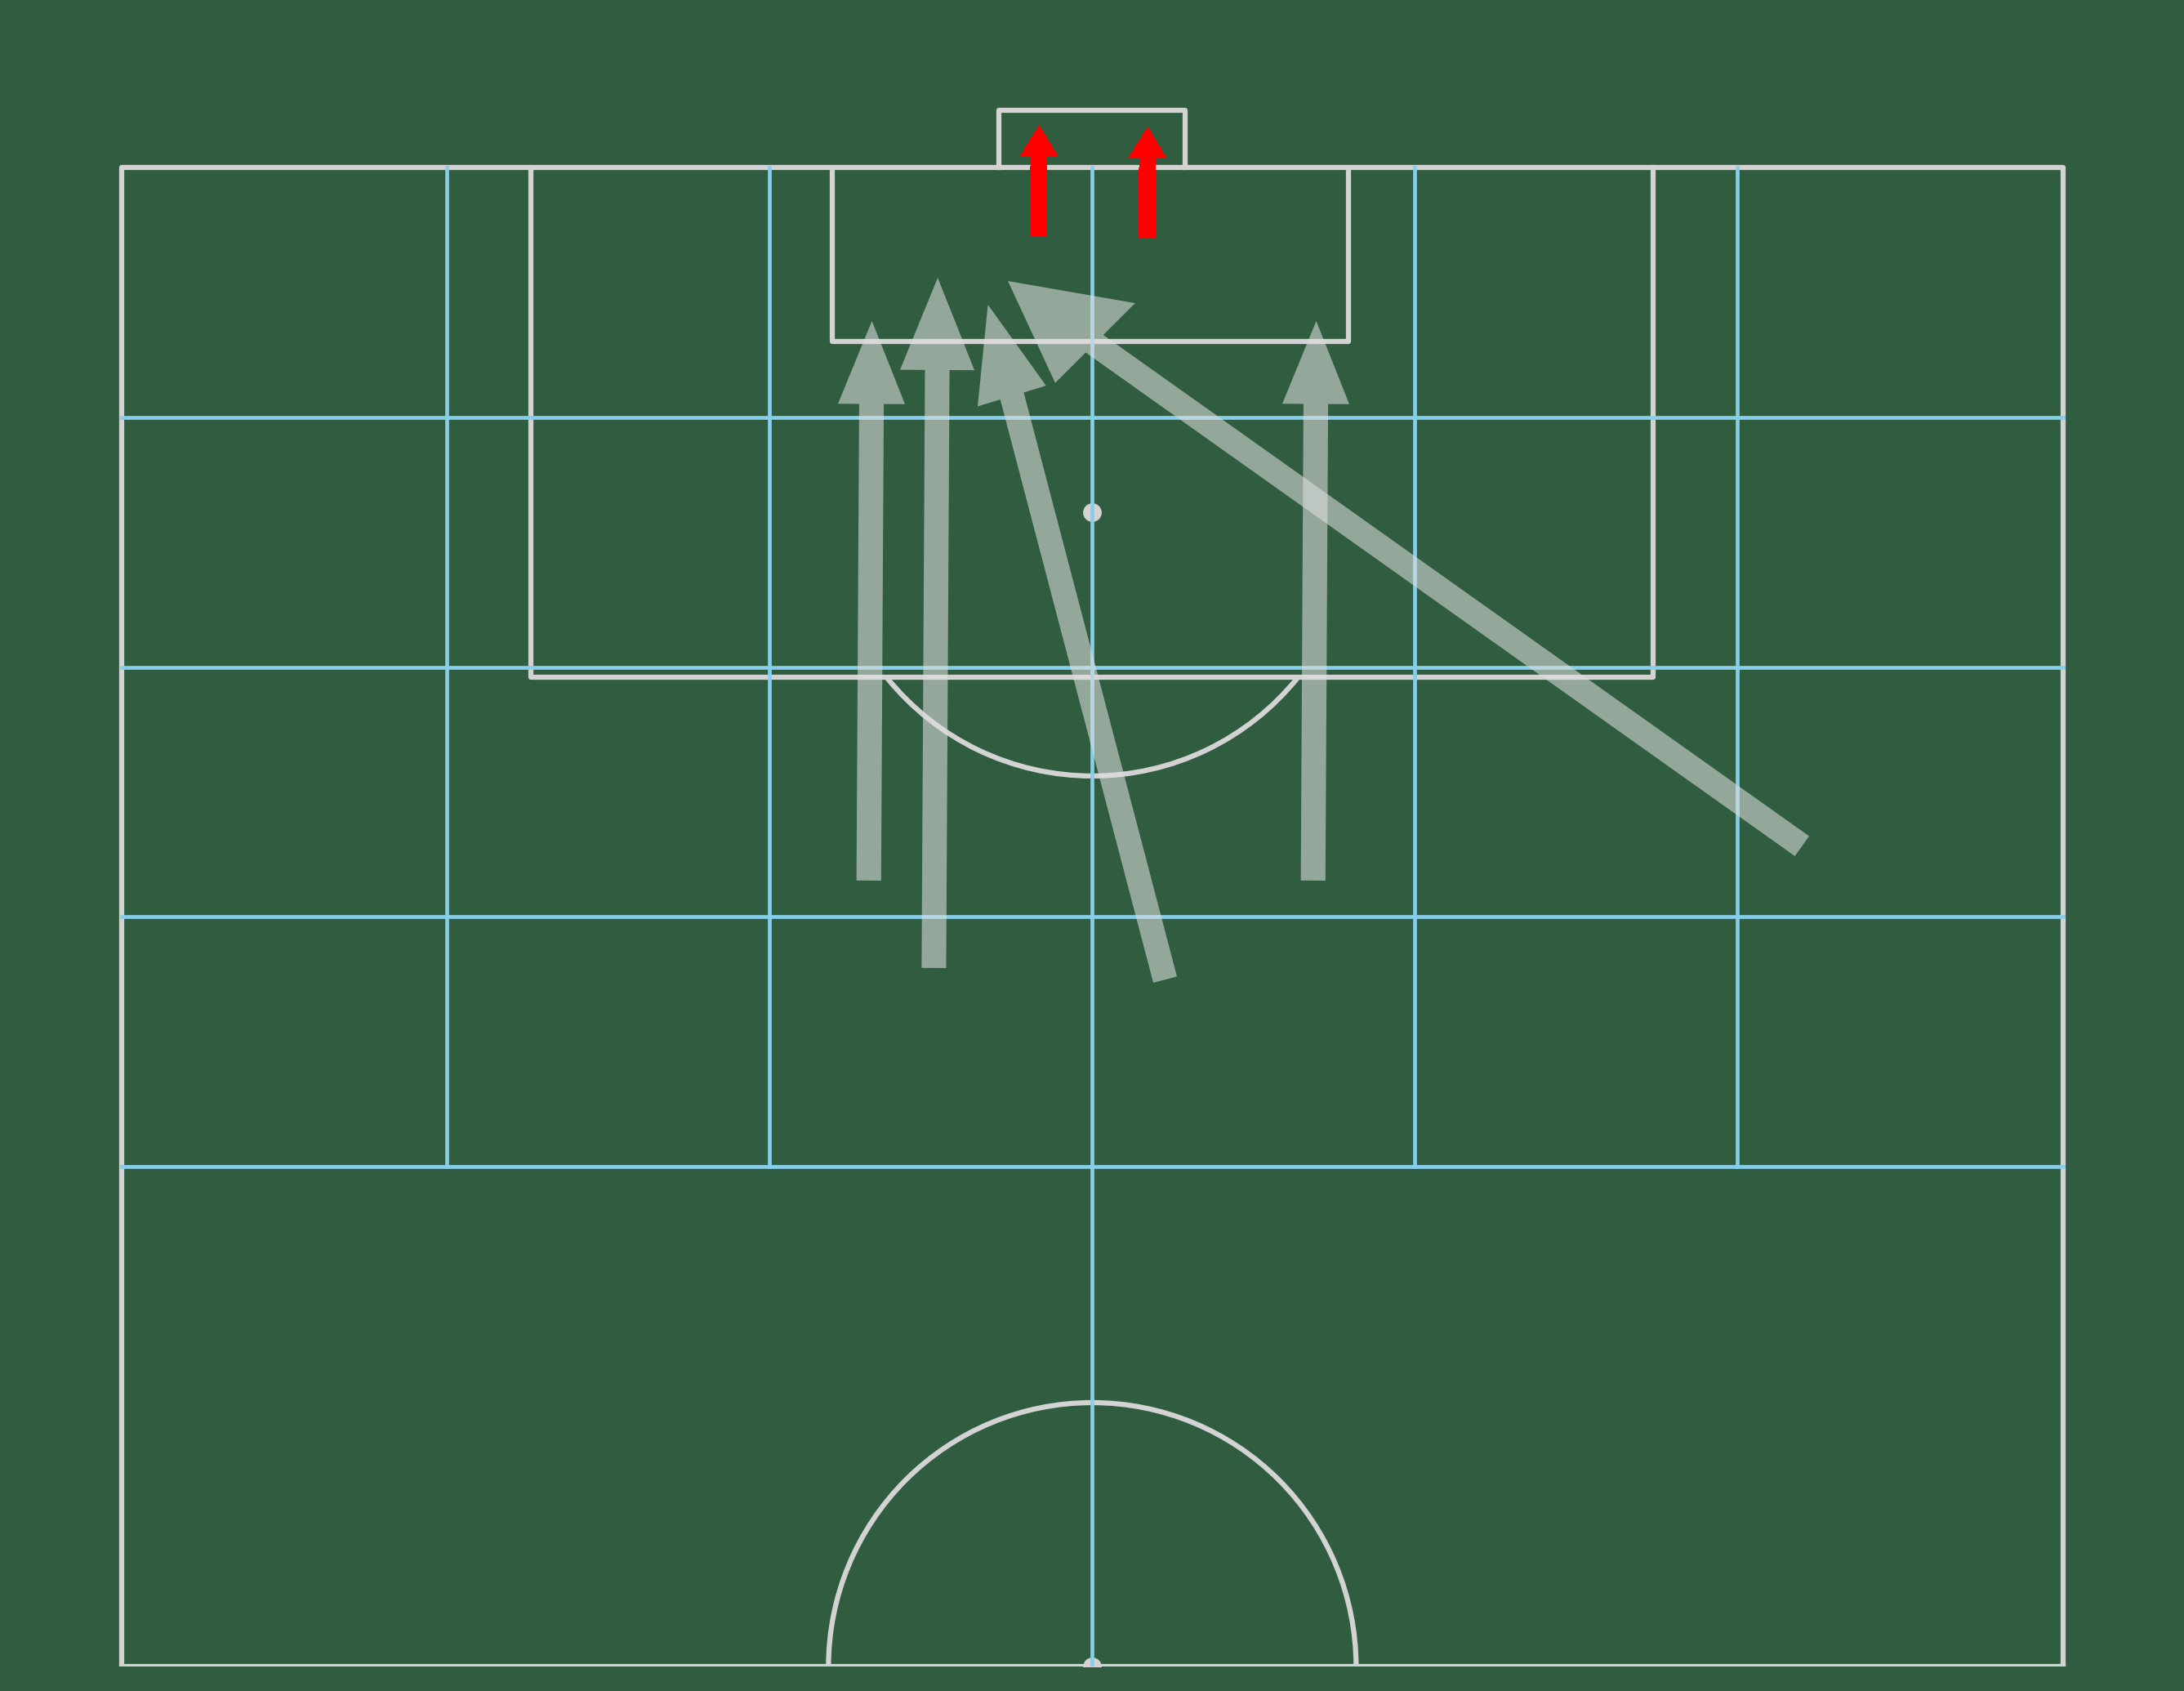
\includegraphics[scale=0.1]{images/earlynthrough.png}   
    \caption{Diagram of optimal passes in attacking play, from early in the attacking third.}
    \label{fig:weezoneearl} 
\end{figure}

This strategy advocates early crosses\footnote{Crosses are flighted passes into the opposition's box.} towards the \textit{back post}, the opposite side of goal from where the pass originates. The long cross from the right wing (\textit{Zone 13}) is again perhaps an indication that there is an abundance of right-footed players in the midfield. 

From more central and advanced areas, the strategy appears to suggest \textit{through balls}, which are passes played through the opposition's defence, usually for an attacking player to run onto. This tactic would require the furthest forward players to be in an onside position when the pass is made - our model, and therefore our strategy, does not account for the positions of defensive players.

The recipients of these crosses and through balls should take the opportunity to shoot, which is unsurprising as the terminal zones (\textit{Zones 22} and \textit{23}) of these actions, or their corresponding states, have the highest average xG values in our model.

\subsection{Refined MDP - ``Back Post!''}

Finally we examine the strategy generated by PRISM for advanced attacking positions. Unsurprisingly, the overriding message is to \textit{"get the ball in the box,"} but the details reveal some interesting insights.

\begin{figure}[htb] 
    \centering
    \begin{subfigure}[b]{0.45\textwidth}
        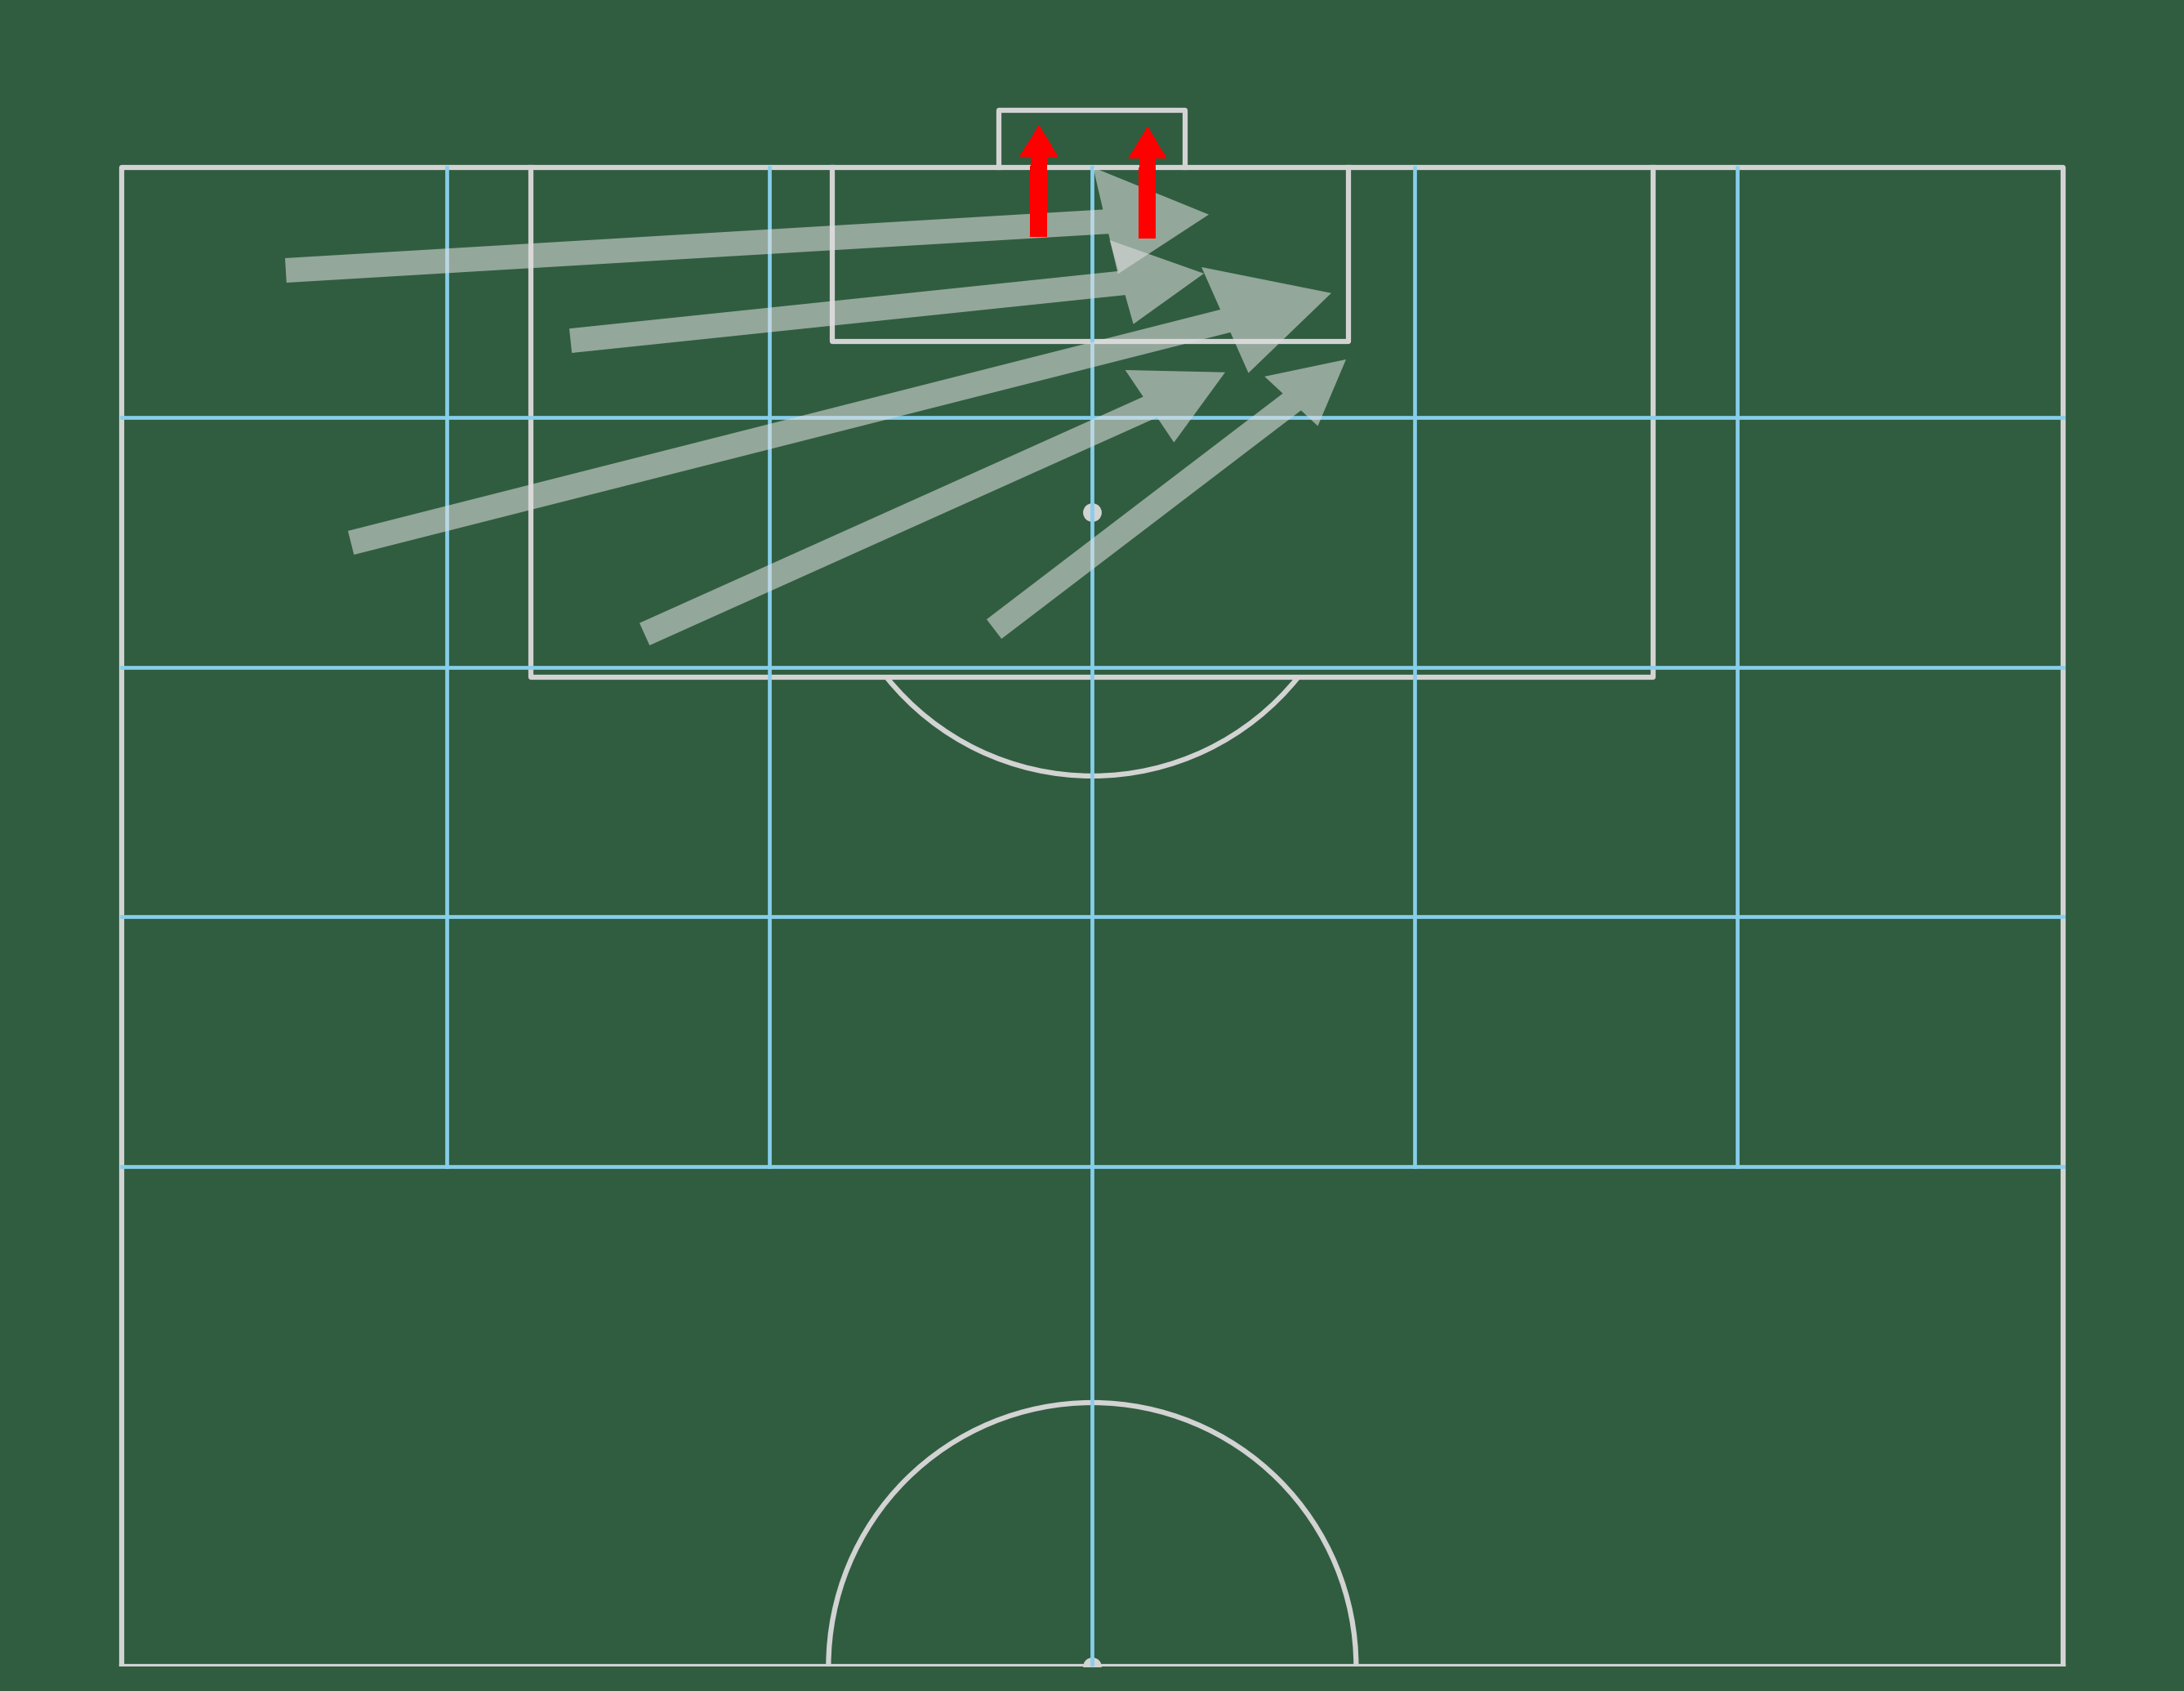
\includegraphics[width=\textwidth]{images/backpostL.png}
        \caption{Optimal actions from an advanced position on the left of the opposition's penalty area.}
        \label{fig:bsticka}
    \end{subfigure}
    ~
    \begin{subfigure}[b]{0.45\textwidth}
        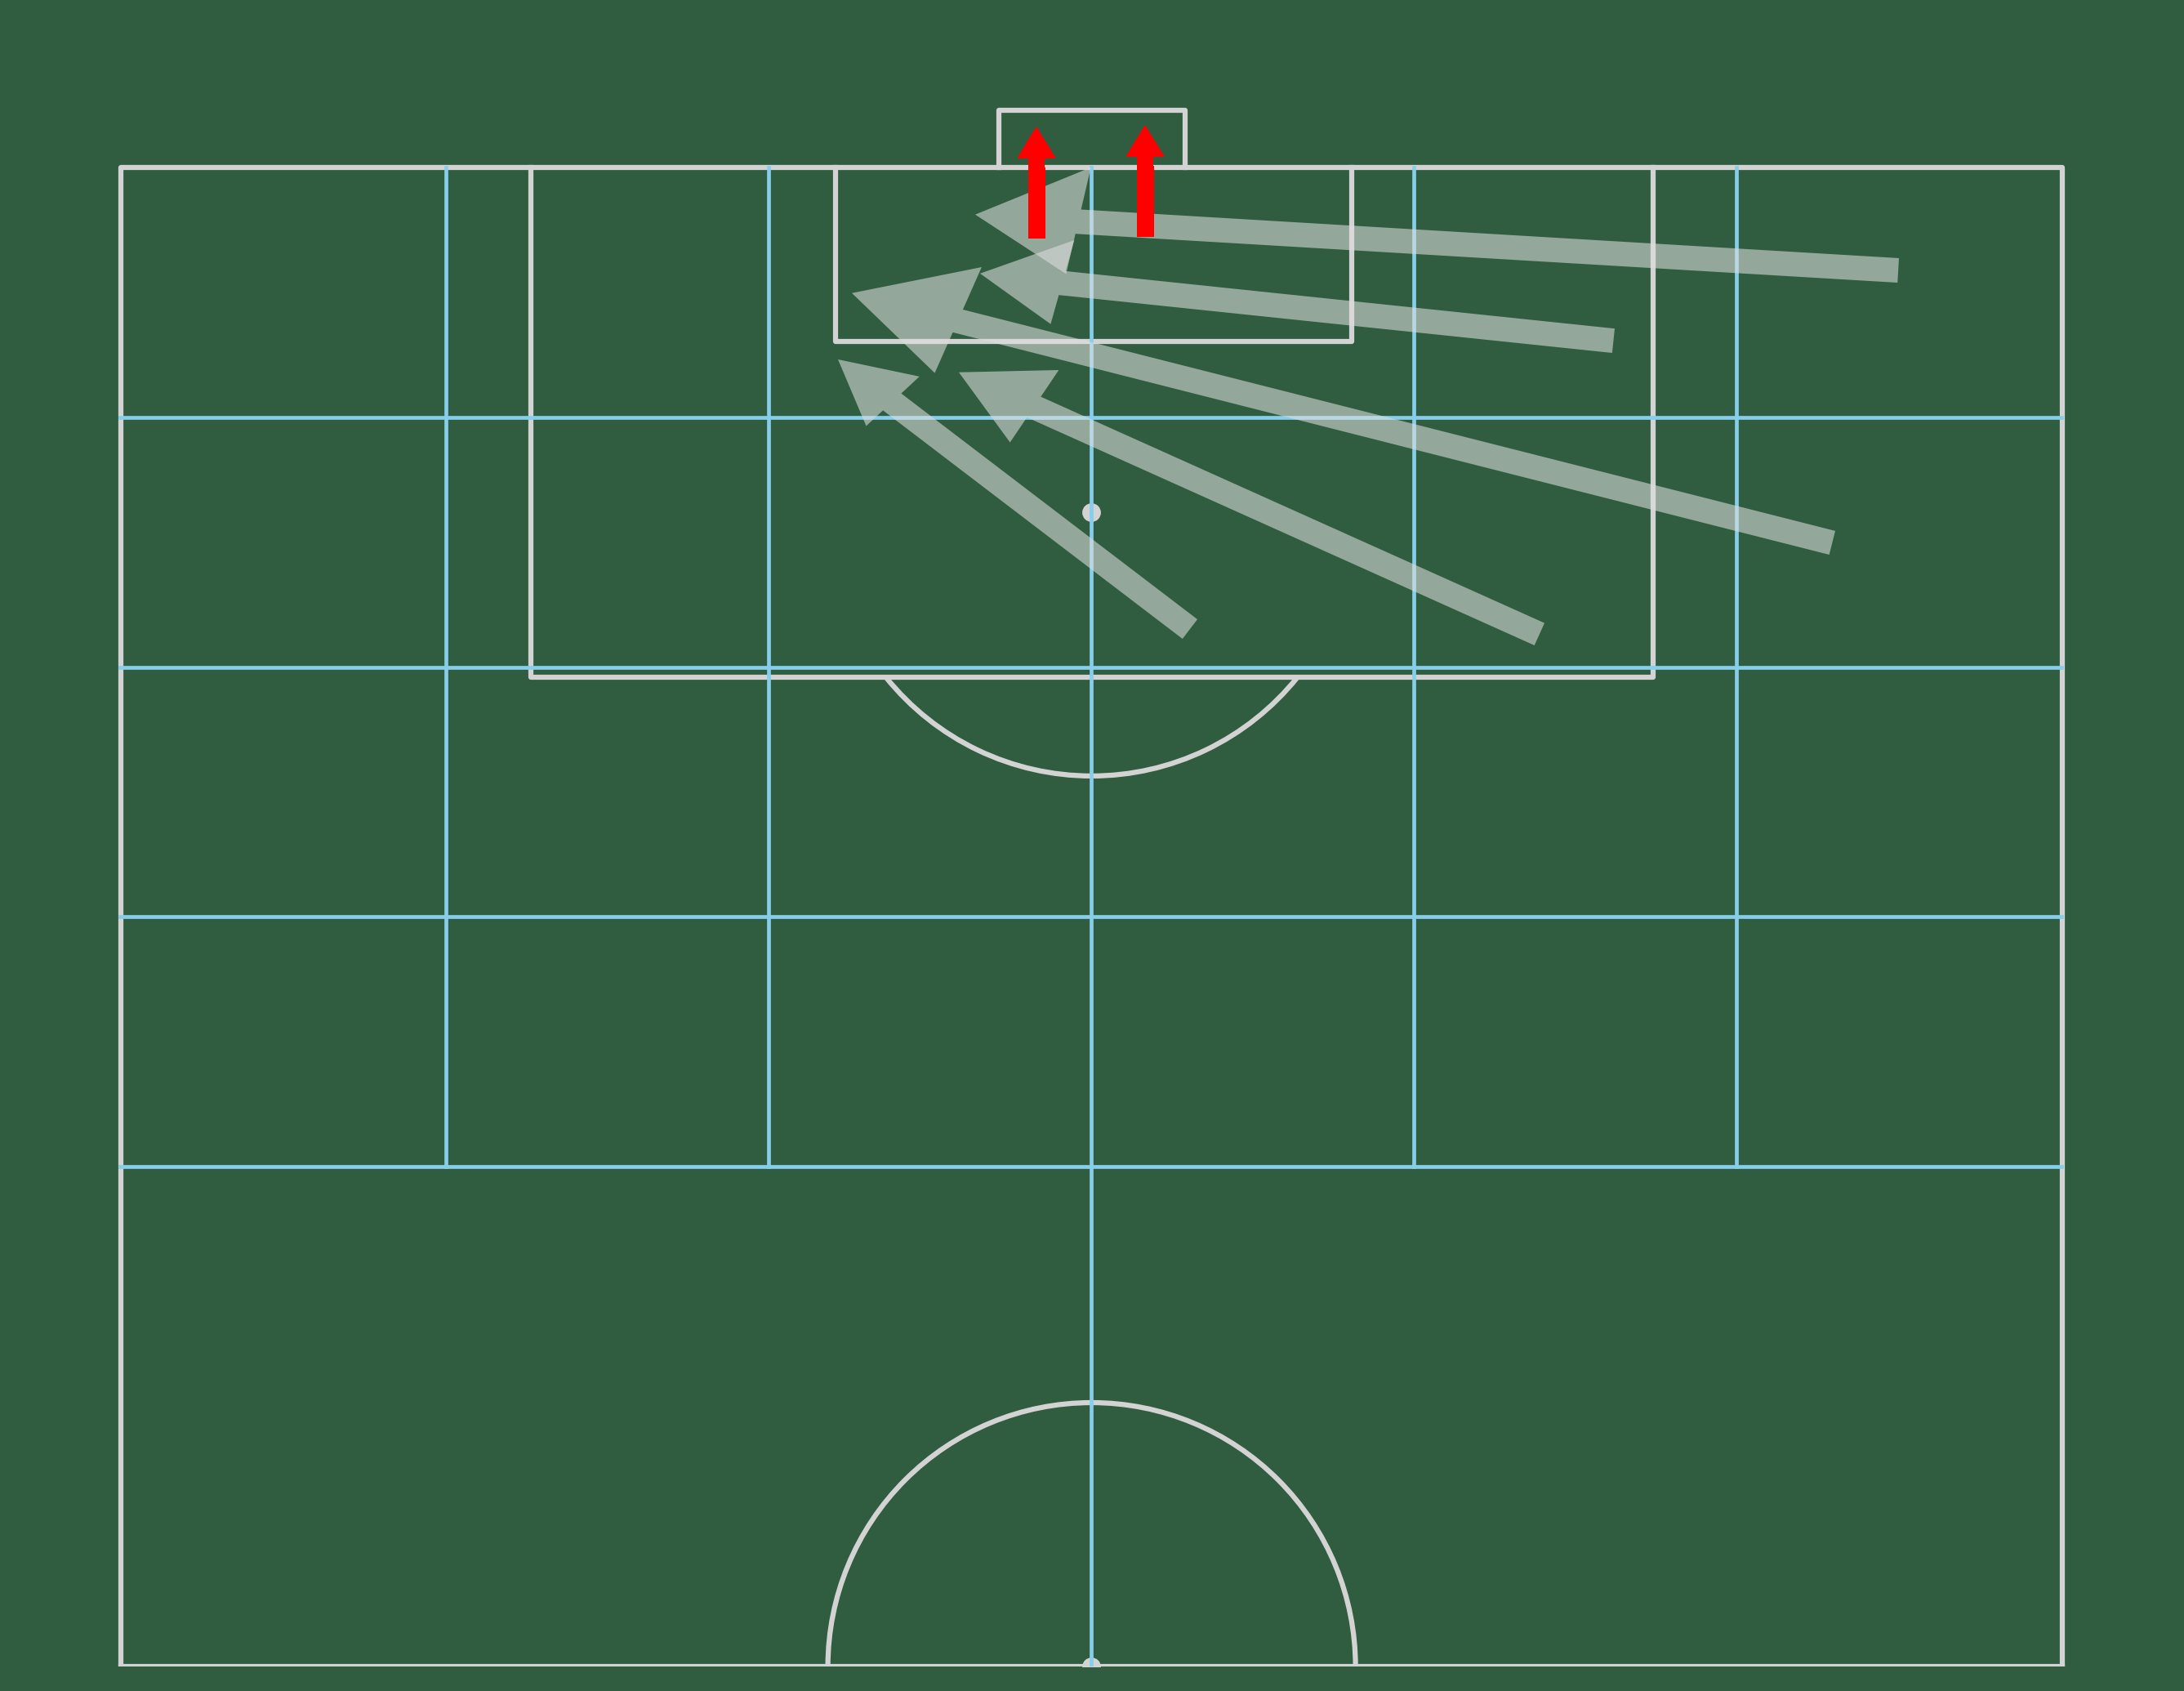
\includegraphics[width=\textwidth]{images/backpostR.png}
        \caption{Optimal actions from an advanced position on the right of the opposition's penalty area.}
        \label{fig:bstickb}
    \end{subfigure}
    ~   
    \caption{\subref{fig:bsticka} and \subref{fig:bstickb} both show that the recommended action is to move the ball towards the opposite side of goal.}
    \label{fig:wzbp}
\end{figure}

\textbf{Fig. \ref{fig:wzbp}} shows the optimal actions deep in the attacking third. From the wings and the outside edges of the box, the best option is to cross the ball to the \textit{back post}; presumably for a waiting team-mate. 

A particularly valuable insight comes from the choices made from either side of the penalty spot (\textit{Zones 16} and \textit{17}). Rather than play the ball forward into the high-xG zones directly in front, the optimal strategy is to play the ball \textit{across the face of goal}.

There are a number of possible reasons for this. With play developing on one side of the box, a goalkeeper may be inclined to move to that side of the goal, leaving the far side exposed. Similarly, defenders may be drawn towards the ball, leaving space in the areas on the other side of the box. Regrettably, without tracking data for opposition players, we won't be able to determine this.

%Design should cover the abstract design in such a way that someone else might be able to do what you did, 
%but with a different language or library or tool. This might include overall system architecture diagrams,
%user interface designs (wireframes/personas/etc.), protocol specifications, algorithms, data set design %choices,
%among others. Specific languages, technical choices, libraries and such like should not usually appear in %the design. These are implementation details.

%==================================================================================================================================
\chapter{Evaluation} 

In the preceding chapters, we have been able to synthesis a plausible strategy for football, using models constructed from event data in conjunction with the PRISM model checker. The strategies generated are at least somewhat interesting, offering more depth than simply, \textit{"get the ball into the box and shoot."}

The strategies we have synthesised are not novel. Building an attack through the middle of the pitch is a common approach in football. Even the more surprising results, calling for the ball to be played back from the box to the edge of midfield, do not represent unusual tactics.

In fact, that these are familiar strategies is very encouraging. From event-level match data, PRISM has been able to synthesise recognisable patterns of play with its optimal adversaries. This suggests that with better data, and more refined models, further insights could be possible.

\section{Limitations}

At the beginning of chapter \ref{limits}, we listed a number of limitations to the data. We chose only to model passes and shots; while this expedited our model construction, the inclusion of dribbles would have offered even more information about how the ball is moved around the pitch. 

We believe that it was right to remove set piece events, although it would be worthwhile to model them separately. Similarly, valuable insights may be possible in modelling actions in a team's own half - either as a preamble to attacking strategy or to examine defensive tactics.

The data we were able to obtain, while extensive, omits a lot of potentially useful information. Off-the-ball team-mate locations would allow us to model the state of an entire team, creating more realistic passing transitions. The same data for the opposition players would allow us to include their positions in the system state, which would undoubtedly have an impact on the optimal strategy for any given configuration of states.

It is particularly unfortunate that our data did not contain match-by-match information about team formations. Synthesising strategies for formation A against formation B may offer genuinely novel solutions for teams facing certain opponents.

In their article about their \textit{Ball Progression Model} \cite{sbomb2}, StatsBomb discussed the limitations of using Markov chains to model football. In particular, they raised questions about the use of \textit{'memoryless'} models when, they argue, probabilistic outcomes in football depend on the manner in which a state was reached. 

We consider that this could be thought of as the result of players (on both teams) finding themselves in certain configurations in the aftermath of certain scenarios. If all of the positional data about players at a given moment can be captured, we can have a single state that is representative of how we arrived at it - we can \textit{infer} the previous state without being reliant upon it, and it is still only the \textit{current} state that affects the probabilistic outcomes.

\section{Improvements}

We propose a number of improvements to the work carried out in this project. Aside from the inclusion of more data points, as discussed above, there is almost certainly scope for better modelling of intent in cases where an action was unsuccessful. Our solution was to assume that unsuccessful passes reached their intended destination. A better approach may be to calculate the zones on the trajectory of the pass, and consider that the pass was intended for any one of them. Of course, if the data included information about intended pass recipients (as StatsBomb's proprietary data does), we would not need to speculate.

Even working with the data we have, our models could be further developed to provide more detailed abstractions of footballing scenarios. We suggest the inclusion of additional modules which could simulate the positions of team-mates and opposition players, or to update a time variable such that we could impose constraints on certain actions.

There are several parts of our Python code that should be refactored for efficiency. As we were not tasked with creating a software product, some best-practices were not as strictly adhered to as they may otherwise be.

%==================================================================================================================================
\chapter{Conclusion}    

Probabilistic model checking has been shown to be a powerful tool for the simulation of very complex systems and the synthesis of strategies for the agents that control them \cite{fac2}. In this study we have made inroads to its application for the analysis of football, and potentially other similar team sports. We have demonstrated that even with a rudimentary model of possession in football, PRISM is capable of generating recognisable, viable strategies for maximum scoring potential, and identified areas where our work can be improved.

\section{Future Work}

Future work that could build immediately upon the work herein could include: refinement of our model building process and the models themselves; extending the models to make use of PRISM's reward structures; verifying the models with more complex properties and queries. We also suggest that data on team formations could drastically increase the value of the insights provided by our methods. 



%==================================================================================================================================
%
%
%==================================================================================================================================
%  APPENDICES  

\begin{appendices}

\chapter{Appendix A}\label{appendix1}


\textbf{Project Specification}

\textit{Model checking for strategy generation in Football}

Co-supervisor: William Kavanagh (PhD student) 

\textbf{Description}:  
This project will involve an investigation into using model checking to identify strategies with maximal scoring potential in football.  

Model checking is a formal technique that allows us to analyse complex systems. An abstract model of the system is created which captures the main features of interest and a tool (model checker) is used to generate a graph (or “state space”) representing all possible behaviours of the system. We can then use the model checker to check properties of our system, which it does by searching the graph using finely tuned search algorithms.  The model is specified using a modelling language such as Promela or Prism – depending on whether properties of interest are qualitative (“event A will occur before event B”, or “event C will eventually happen”) or quantitative (“event A will eventually happen with probability p”, or “in the long term the expected reward is R”) and properties are specified using an appropriate temporal logic, then checked using a model checker such as SPIN [1] or PRISM [2]. Model checking is the main subject covered in the H/M level course, “Modelling Reactive Systems” (MRS). 

Football analysis has vastly improved over recent years with the introduction of advanced metrics. The most prominent of these is expected goals, xG [3]. The xG of any shot taken in a football match is the probability of a goal, calculated by studying all similar shots taken by professional footballs within a defined recent time window. A recent paper [4] discusses the use of xG as a tool for combatting randomness in football.  

In this project you will: 
\begin{itemize}
    \item synthesise player data (possibly extracted from match footage) 
    \item determine xG data for different shots (determined by position on the field of the shooter/positions of other players etc.)
    \item using your synthesised data:
    \begin{itemize}
        \item develop PRISM models in which players choose actions with probabilistic outcomes, (where probabilities are based on your synthesised data) 
        \item use the PRISM model checker to automatically determine strategies from fixed player states which are optimal in terms of expected number of goals scored within a defined time limit.  
        \end{itemize}
    \end{itemize}
    
Attendance at Dr Oana Andrei’s MRS course is strongly advised, and attendance at Constraint Programming (CP) and Machine Learning (ML) would be useful.  

[1] The Spin Model Checker, G. Holzmann, Addison Wesley, 2003.  

[2] PRISM model checker, http://www.prismmodelchecker.org/  

[3] No seriously, what the heck is expected goals (xG)?	 https://www.fourfourtwo.com/features/no-seriously-what-heck-expected-goals-xg 

[4] Brechot, M. and Flepp, R. Dealing with randomness in match outcomes: How to rethink performance evaluation in European club football using expected goals. Journal of Sports Economics 21 (4), pp 335-362.  

Special Requirements: will need access to free model checking software (Spin, Prism) 
    
\chapter{Appendix B}\label{lst:appendix2}
\begin{lstlisting}[language=Haskell, numbers=left, caption=Initial DTMC specification in the PRISM modelling language.] 
    dtmc
    module possession

	// state: i.e. area of the pitch where ball is in possession
	s : [0..8];
		// 0 - 6: areas of the pitch
		// 7    : possession lost
		// 8    : goal scored

	[] s=0 -> 0.49970679072676805 : (s'=0) + 0.11243297536741377  : (s'=1) + 0.06151981643595859  : (s'=2) + 0.11160296757857256  : (s'=3) + 0.020193848920538784  : (s'=4) + 0.005906287309000472  : (s'=5) + 0.021971148207513978  : (s'=6) + 0.1666360927082613  : (s'=7) + 3.0072745972507496e-05  : (s'=8);
	[] s=1 -> 0.18713713187118003 : (s'=0) + 0.2773245081253766  : (s'=1) + 0.07777214511855685  : (s'=2) + 0.010569206783422127  : (s'=3) + 0.11936986484806167  : (s'=4) + 0.03541879884073497  : (s'=5) + 0.010435298281188724  : (s'=6) + 0.28146610680159545  : (s'=7) + 0.0005069393298835952  : (s'=8);
	[] s=2 -> 0.09408800986225009 : (s'=0) + 0.06593771774669024  : (s'=1) + 0.1368923192367476  : (s'=2) + 0.06804952564721016  : (s'=3) + 0.03657608404352254  : (s'=4) + 0.0302406603419628  : (s'=5) + 0.04112129495631667  : (s'=6) + 0.5228064533419092  : (s'=7) + 0.004287934823390685  : (s'=8);
	[] s=3 -> 0.1830642440599548 : (s'=0) + 0.009243818979227915  : (s'=1) + 0.0739601908525712  : (s'=2) + 0.2831365367005639  : (s'=3) + 0.009957106366571883  : (s'=4) + 0.03943322569762398  : (s'=5) + 0.12725432550966312  : (s'=6) + 0.27360354715889923  : (s'=7) + 0.00034700467492409273  : (s'=8);
	[] s=4 -> 0.009141108100841726 : (s'=0) + 0.11895849275122536  : (s'=1) + 0.02063987756705892  : (s'=2) + 0.0031228672471201374  : (s'=3) + 0.12661055156867207  : (s'=4) + 0.11244390213637209  : (s'=5) + 0.015924554836307985  : (s'=6) + 0.5892705726635369  : (s'=7) + 0.0038880731288648065  : (s'=8);
	[] s=5 -> 0.0003603517032623841  : (s'=0) + 0.0012492192379762648  : (s'=1) + 0.00838418296257147  : (s'=2) + 0.0015375006005861722  : (s'=3) + 0.004444337673569404  : (s'=4) + 0.021681160812953442  : (s'=5) + 0.00454043146110604  : (s'=6) + 0.916866862057368  : (s'=7) + 0.04093595349060683  : (s'=8);
	[] s=6 -> 0.009717038180036282 : (s'=0) + 0.0035239902412577935  : (s'=1) + 0.018495735763287946  : (s'=2) + 0.11841858331421899  : (s'=3) + 0.016910982755385034  : (s'=4) + 0.12436140709385492  : (s'=5) + 0.12888629397168297  : (s'=6) + 0.5760994223992326  : (s'=7) + 0.0035865462810434345  : (s'=8);

	// absorbing states
	[] s=7 -> (s'=7);
	[] s=8 -> (s'=8);

    endmodule

    const int x;

    init s=x endinit;

    label "possession_lost" = (s=7);
    label "goal" = (s=8);
    \end{lstlisting}

\chapter{Appendix C}\label{appendix3}

\begin{lstlisting}[language=Haskell, numbers=left, caption=Initial MDP specification in the PRISM modelling language.] 
mdp

module passes_and_shots

	// states: 0-6 = zones on the pitch; 7 = possession lost; 8 = goal scored
	s : [0..8];
	// player actions from zone 0 (s=0)
	[pass_0_0]	      s=0 ->
	0.9055121113866107 : (s'=0) + (1 - 0.9055121113866107) : (s'=7);
	[pass_0_1]	      s=0 ->
	0.8096805630752572 : (s'=1) + (1 - 0.8096805630752572) : (s'=7);
	[pass_0_2]	      s=0 ->
	0.7466875935321385 : (s'=2) + (1 - 0.7466875935321385) : (s'=7);
	[pass_0_3]	      s=0 ->
	0.8102130818269146 : (s'=3) + (1 - 0.8102130818269146) : (s'=7);
	[pass_0_4]	      s=0 ->
	0.6955666045162627 : (s'=4) + (1 - 0.6955666045162627) : (s'=7);
	[pass_0_5]	      s=0 ->
	0.3562488663159804 : (s'=5) + (1 - 0.3562488663159804) : (s'=7);
	[pass_0_6]	      s=0 ->
	0.6746698679471789 : (s'=6) + (1 - 0.6746698679471789) : (s'=7);
	[shoot_0]	       s=0 ->
	0.007867820613690008 : (s'=8) + (1 - 0.007867820613690008) : (s'=7);

	// player actions from zone 1 (s=1)
	[pass_1_0]	      s=1 ->
	0.9377396472392638 : (s'=0) + (1 - 0.9377396472392638) : (s'=7);
	[pass_1_1]	      s=1 ->
	0.8372992953679104 : (s'=1) + (1 - 0.8372992953679104) : (s'=7);
	[pass_1_2]	      s=1 ->
	0.8151378446115288 : (s'=2) + (1 - 0.8151378446115288) : (s'=7);
	[pass_1_3]	      s=1 ->
	0.7984104046242775 : (s'=3) + (1 - 0.7984104046242775) : (s'=7);
	[pass_1_4]	      s=1 ->
	0.7862407862407862 : (s'=4) + (1 - 0.7862407862407862) : (s'=7);
	[pass_1_5]	      s=1 ->
	0.43760340345072085 : (s'=5) + (1 - 0.43760340345072085) : (s'=7);
	[pass_1_6]	      s=1 ->
	0.40876732858748593 : (s'=6) + (1 - 0.40876732858748593) : (s'=7);
	[shoot_1]	       s=1 ->
	0.005434225366553881 : (s'=8) + (1 - 0.005434225366553881) : (s'=7);

	// player actions from zone 2 (s=2)
	[pass_2_0]	      s=2 ->
	0.9249657498155759 : (s'=0) + (1 - 0.9249657498155759) : (s'=7);
	[pass_2_1]	      s=2 ->
	0.8348262757871878 : (s'=1) + (1 - 0.8348262757871878) : (s'=7);
	[pass_2_2]	      s=2 ->
	0.7675201346315663 : (s'=2) + (1 - 0.7675201346315663) : (s'=7);
	[pass_2_3]	      s=2 ->
	0.8424684804246848 : (s'=3) + (1 - 0.8424684804246848) : (s'=7);
	[pass_2_4]	      s=2 ->
	0.7921987462270722 : (s'=4) + (1 - 0.7921987462270722) : (s'=7);
	[pass_2_5]	      s=2 ->
	0.522697795071336 : (s'=5) + (1 - 0.522697795071336) : (s'=7);
	[pass_2_6]	      s=2 ->
	0.8040243135610983 : (s'=6) + (1 - 0.8040243135610983) : (s'=7);
	[shoot_2]	       s=2 ->
	0.010622477161674103 : (s'=8) + (1 - 0.010622477161674103) : (s'=7);

	// player actions from zone 3 (s=3)
	[pass_3_0]	      s=3 ->
	0.9333595439355219 : (s'=0) + (1 - 0.9333595439355219) : (s'=7);
	[pass_3_1]	      s=3 ->
	0.7899505766062603 : (s'=1) + (1 - 0.7899505766062603) : (s'=7);
	[pass_3_2]	      s=3 ->
	0.8004381389526393 : (s'=2) + (1 - 0.8004381389526393) : (s'=7);
	[pass_3_3]	      s=3 ->
	0.8351767080833641 : (s'=3) + (1 - 0.8351767080833641) : (s'=7);
	[pass_3_4]	      s=3 ->
	0.5240994419076611 : (s'=4) + (1 - 0.5240994419076611) : (s'=7);
	[pass_3_5]	      s=3 ->
	0.4531457687195392 : (s'=5) + (1 - 0.4531457687195392) : (s'=7);
	[pass_3_6]	      s=3 ->
	0.7505400795906765 : (s'=6) + (1 - 0.7505400795906765) : (s'=7);
	[shoot_3]	       s=3 ->
	0.004558693174623275 : (s'=8) + (1 - 0.004558693174623275) : (s'=7);

	// player actions from zone 4 (s=4)
	[pass_4_0]	      s=4 ->
	0.8403041825095057 : (s'=0) + (1 - 0.8403041825095057) : (s'=7);
	[pass_4_1]	      s=4 ->
	0.9075418112969391 : (s'=1) + (1 - 0.9075418112969391) : (s'=7);
	[pass_4_2]	      s=4 ->
	0.7641653905053599 : (s'=2) + (1 - 0.7641653905053599) : (s'=7);
	[pass_4_3]	      s=4 ->
	0.44807121661721067 : (s'=3) + (1 - 0.44807121661721067) : (s'=7);
	[pass_4_4]	      s=4 ->
	0.6910486510892877 : (s'=4) + (1 - 0.6910486510892877) : (s'=7);
	[pass_4_5]	      s=4 ->
	0.43635634028892456 : (s'=5) + (1 - 0.43635634028892456) : (s'=7);
	[pass_4_6]	      s=4 ->
	0.2033271719038817 : (s'=6) + (1 - 0.2033271719038817) : (s'=7);
	[shoot_4]	       s=4 ->
	0.01550131926121372 : (s'=8) + (1 - 0.01550131926121372) : (s'=7);

	// player actions from zone 5 (s=5)
	[pass_5_0]	      s=5 ->
	0.8108108108108109 : (s'=0) + (1 - 0.8108108108108109) : (s'=7);
	[pass_5_1]	      s=5 ->
	0.7074829931972789 : (s'=1) + (1 - 0.7074829931972789) : (s'=7);
	[pass_5_2]	      s=5 ->
	0.8050749711649365 : (s'=2) + (1 - 0.8050749711649365) : (s'=7);
	[pass_5_3]	      s=5 ->
	0.7485380116959064 : (s'=3) + (1 - 0.7485380116959064) : (s'=7);
	[pass_5_4]	      s=5 ->
	0.6368330464716007 : (s'=4) + (1 - 0.6368330464716007) : (s'=7);
	[pass_5_5]	      s=5 ->
	0.5706607650964275 : (s'=5) + (1 - 0.5706607650964275) : (s'=7);
	[pass_5_6]	      s=5 ->
	0.6009538950715422 : (s'=6) + (1 - 0.6009538950715422) : (s'=7);
	[shoot_5]	       s=5 ->
	0.04394754149096677 : (s'=8) + (1 - 0.04394754149096677) : (s'=7);

	// player actions from zone 6 (s=6)
	[pass_6_0]	      s=6 ->
	0.8677839851024208 : (s'=0) + (1 - 0.8677839851024208) : (s'=7);
	[pass_6_1]	      s=6 ->
	0.4412532637075718 : (s'=1) + (1 - 0.4412532637075718) : (s'=7);
	[pass_6_2]	      s=6 ->
	0.7472620050547599 : (s'=2) + (1 - 0.7472620050547599) : (s'=7);
	[pass_6_3]	      s=6 ->
	0.9098045498237745 : (s'=3) + (1 - 0.9098045498237745) : (s'=7);
	[pass_6_4]	      s=6 ->
	0.43578721117678665 : (s'=4) + (1 - 0.43578721117678665) : (s'=7);
	[pass_6_5]	      s=6 ->
	0.44190871369294604 : (s'=5) + (1 - 0.44190871369294604) : (s'=7);
	[pass_6_6]	      s=6 ->
	0.5506458797327394 : (s'=6) + (1 - 0.5506458797327394) : (s'=7);
	[shoot_6]	       s=6 ->
	0.016736401673640166 : (s'=8) + (1 - 0.016736401673640166) : (s'=7);

	// absorbing states
	[] s=7 -> (s'=7);
	[] s=8 -> (s'=8);

endmodule

label "ball_in_zone_0" = (s=0);
label "ball_in_zone_1" = (s=1);
label "ball_in_zone_2" = (s=2);
label "ball_in_zone_3" = (s=3);
label "ball_in_zone_4" = (s=4);
label "ball_in_zone_5" = (s=5);
label "ball_in_zone_6" = (s=6);
label "possession_lost" = (s=7);
label "goal" = (s=8);

\end{lstlisting}

\chapter{Appendix D}\label{appendix4}

\begin{lstlisting}[language=Haskell, numbers=left, caption=MDP used for strategy generation. This is the model specification as-is after the refinements at the end of chapter 3.] 
mdp

module passes_and_shots

	// states: 0-6 = zones on the pitch; 7 = possession lost; 8 = goal scored
	s : [0..27];
	// player actions from zone 0 (s=0)
	[pass_0_0]	      s=0 ->
	0.8986493560883677 : (s'=0) + (1 - 0.8986493560883677) : (s'=26);
	[pass_0_1]	      s=0 ->
	0.9450302894323536 : (s'=1) + (1 - 0.9450302894323536) : (s'=26);
	[pass_0_2]	      s=0 ->
	0.8515671790776602 : (s'=2) + (1 - 0.8515671790776602) : (s'=26);
	[pass_0_3]	      s=0 ->
	0.791751735402205 : (s'=3) + (1 - 0.791751735402205) : (s'=26);
	[pass_0_4]	      s=0 ->
	0.7853581737076882 : (s'=4) + (1 - 0.7853581737076882) : (s'=26);
	[pass_0_5]	      s=0 ->
	0.7909140667761357 : (s'=5) + (1 - 0.7909140667761357) : (s'=26);
	[pass_0_6]	      s=0 ->
	0.7967213114754098 : (s'=6) + (1 - 0.7967213114754098) : (s'=26);
	[pass_0_7]	      s=0 ->
	0.8561307901907357 : (s'=7) + (1 - 0.8561307901907357) : (s'=26);
	[pass_0_8]	      s=0 ->
	0.8123775310254735 : (s'=8) + (1 - 0.8123775310254735) : (s'=26);
	[pass_0_9]	      s=0 ->
	0.6439516129032258 : (s'=9) + (1 - 0.6439516129032258) : (s'=26);
	[pass_0_10]	      s=0 ->
	0.5806233062330624 : (s'=10) + (1 - 0.5806233062330624) : (s'=26);
	[pass_0_11]	      s=0 ->
	0.5850931677018634 : (s'=11) + (1 - 0.5850931677018634) : (s'=26);
	[pass_0_12]	      s=0 ->
	0.6214177978883861 : (s'=12) + (1 - 0.6214177978883861) : (s'=26);
	[pass_0_13]	      s=0 ->
	0.7881873727087576 : (s'=13) + (1 - 0.7881873727087576) : (s'=26);
	[pass_0_14]	      s=0 ->
	0.7824624935333678 : (s'=14) + (1 - 0.7824624935333678) : (s'=26);
	[pass_0_15]	      s=0 ->
	0.6670428893905191 : (s'=15) + (1 - 0.6670428893905191) : (s'=26);
	[pass_0_16]	      s=0 ->
	0.32379623168178645 : (s'=16) + (1 - 0.32379623168178645) : (s'=26);
	[pass_0_17]	      s=0 ->
	0.42960662525879917 : (s'=17) + (1 - 0.42960662525879917) : (s'=26);
	[pass_0_18]	      s=0 ->
	0.6758104738154613 : (s'=18) + (1 - 0.6758104738154613) : (s'=26);
	[pass_0_19]	      s=0 ->
	0.8137142857142857 : (s'=19) + (1 - 0.8137142857142857) : (s'=26);
	[pass_0_20]	      s=0 ->
	0.5903010033444817 : (s'=20) + (1 - 0.5903010033444817) : (s'=26);
	[pass_0_21]	      s=0 ->
	0.5443959243085881 : (s'=21) + (1 - 0.5443959243085881) : (s'=26);
	[pass_0_22]	      s=0 ->
	0.22377622377622378 : (s'=22) + (1 - 0.22377622377622378) : (s'=26);
	[pass_0_23]	      s=0 ->
	0.3069306930693069 : (s'=23) + (1 - 0.3069306930693069) : (s'=26);
	[pass_0_24]	      s=0 ->
	0.4938650306748466 : (s'=24) + (1 - 0.4938650306748466) : (s'=26);
	[pass_0_25]	      s=0 ->
	0.4745484400656814 : (s'=25) + (1 - 0.4745484400656814) : (s'=26);
	[shoot_0]	       s=0 ->
	0.007407407407407408 : (s'=27) + (1 - 0.007407407407407408) : (s'=26);

	// player actions from zone 1 (s=1)
	[pass_1_0]	      s=1 ->
	0.9414324154119196 : (s'=0) + (1 - 0.9414324154119196) : (s'=26);
	[pass_1_1]	      s=1 ->
	0.8942647837107601 : (s'=1) + (1 - 0.8942647837107601) : (s'=26);
	[pass_1_2]	      s=1 ->
	0.8338762214983714 : (s'=2) + (1 - 0.8338762214983714) : (s'=26);
	[pass_1_3]	      s=1 ->
	0.7592592592592593 : (s'=3) + (1 - 0.7592592592592593) : (s'=26);
	[pass_1_4]	      s=1 ->
	0.7827724761426419 : (s'=4) + (1 - 0.7827724761426419) : (s'=26);
	[pass_1_5]	      s=1 ->
	0.7746763754045307 : (s'=5) + (1 - 0.7746763754045307) : (s'=26);
	[pass_1_6]	      s=1 ->
	0.7982648057336854 : (s'=6) + (1 - 0.7982648057336854) : (s'=26);
	[pass_1_7]	      s=1 ->
	0.8480190517428015 : (s'=7) + (1 - 0.8480190517428015) : (s'=26);
	[pass_1_8]	      s=1 ->
	0.7656078860898138 : (s'=8) + (1 - 0.7656078860898138) : (s'=26);
	[pass_1_9]	      s=1 ->
	0.6015503875968993 : (s'=9) + (1 - 0.6015503875968993) : (s'=26);
	[pass_1_10]	      s=1 ->
	0.5774793388429752 : (s'=10) + (1 - 0.5774793388429752) : (s'=26);
	[pass_1_11]	      s=1 ->
	0.5644504748982361 : (s'=11) + (1 - 0.5644504748982361) : (s'=26);
	[pass_1_12]	      s=1 ->
	0.6481060606060606 : (s'=12) + (1 - 0.6481060606060606) : (s'=26);
	[pass_1_13]	      s=1 ->
	0.8052505147563487 : (s'=13) + (1 - 0.8052505147563487) : (s'=26);
	[pass_1_14]	      s=1 ->
	0.793733681462141 : (s'=14) + (1 - 0.793733681462141) : (s'=26);
	[pass_1_15]	      s=1 ->
	0.6547770700636942 : (s'=15) + (1 - 0.6547770700636942) : (s'=26);
	[pass_1_16]	      s=1 ->
	0.37823022709475335 : (s'=16) + (1 - 0.37823022709475335) : (s'=26);
	[pass_1_17]	      s=1 ->
	0.35730337078651686 : (s'=17) + (1 - 0.35730337078651686) : (s'=26);
	[pass_1_18]	      s=1 ->
	0.645822102425876 : (s'=18) + (1 - 0.645822102425876) : (s'=26);
	[pass_1_19]	      s=1 ->
	0.788768675940237 : (s'=19) + (1 - 0.788768675940237) : (s'=26);
	[pass_1_20]	      s=1 ->
	0.5898305084745763 : (s'=20) + (1 - 0.5898305084745763) : (s'=26);
	[pass_1_21]	      s=1 ->
	0.45993031358885017 : (s'=21) + (1 - 0.45993031358885017) : (s'=26);
	[pass_1_22]	      s=1 ->
	0.3178294573643411 : (s'=22) + (1 - 0.3178294573643411) : (s'=26);
	[pass_1_23]	      s=1 ->
	0.16279069767441862 : (s'=23) + (1 - 0.16279069767441862) : (s'=26);
	[pass_1_24]	      s=1 ->
	0.5757918552036199 : (s'=24) + (1 - 0.5757918552036199) : (s'=26);
	[pass_1_25]	      s=1 ->
	0.5219298245614035 : (s'=25) + (1 - 0.5219298245614035) : (s'=26);
	[shoot_1]	       s=1 ->
	0.008532423208191127 : (s'=27) + (1 - 0.008532423208191127) : (s'=26);

	// player actions from zone 2 (s=2)
	[pass_2_0]	      s=2 ->
	0.9384417808219178 : (s'=0) + (1 - 0.9384417808219178) : (s'=26);
	[pass_2_1]	      s=2 ->
	0.9050847457627119 : (s'=1) + (1 - 0.9050847457627119) : (s'=26);
	[pass_2_2]	      s=2 ->
	0.805713358221068 : (s'=2) + (1 - 0.805713358221068) : (s'=26);
	[pass_2_3]	      s=2 ->
	0.8836104513064132 : (s'=3) + (1 - 0.8836104513064132) : (s'=26);
	[pass_2_4]	      s=2 ->
	0.8595555555555555 : (s'=4) + (1 - 0.8595555555555555) : (s'=26);
	[pass_2_5]	      s=2 ->
	0.8232558139534883 : (s'=5) + (1 - 0.8232558139534883) : (s'=26);
	[pass_2_6]	      s=2 ->
	0.7228915662650602 : (s'=6) + (1 - 0.7228915662650602) : (s'=26);
	[pass_2_7]	      s=2 ->
	0.7843137254901961 : (s'=7) + (1 - 0.7843137254901961) : (s'=26);
	[pass_2_8]	      s=2 ->
	0.8135874067937034 : (s'=8) + (1 - 0.8135874067937034) : (s'=26);
	[pass_2_9]	      s=2 ->
	0.7404411764705883 : (s'=9) + (1 - 0.7404411764705883) : (s'=26);
	[pass_2_10]	      s=2 ->
	0.6538461538461539 : (s'=10) + (1 - 0.6538461538461539) : (s'=26);
	[pass_2_11]	      s=2 ->
	0.5416666666666666 : (s'=11) + (1 - 0.5416666666666666) : (s'=26);
	[pass_2_12]	      s=2 ->
	0.7073170731707317 : (s'=12) + (1 - 0.7073170731707317) : (s'=26);
	[pass_2_13]	      s=2 ->
	0.5714285714285714 : (s'=13) + (1 - 0.5714285714285714) : (s'=26);
	[pass_2_14]	      s=2 ->
	0.8290506780870807 : (s'=14) + (1 - 0.8290506780870807) : (s'=26);
	[pass_2_15]	      s=2 ->
	0.6859956236323851 : (s'=15) + (1 - 0.6859956236323851) : (s'=26);
	[pass_2_16]	      s=2 ->
	0.3865220759101472 : (s'=16) + (1 - 0.3865220759101472) : (s'=26);
	[pass_2_17]	      s=2 ->
	0.49171270718232046 : (s'=17) + (1 - 0.49171270718232046) : (s'=26);
	[pass_2_18]	      s=2 ->
	0.5232558139534884 : (s'=18) + (1 - 0.5232558139534884) : (s'=26);
	[pass_2_19]	      s=2 ->
	0.5681818181818182 : (s'=19) + (1 - 0.5681818181818182) : (s'=26);
	[pass_2_20]	      s=2 ->
	0.7752027809965237 : (s'=20) + (1 - 0.7752027809965237) : (s'=26);
	[pass_2_21]	      s=2 ->
	0.7186147186147186 : (s'=21) + (1 - 0.7186147186147186) : (s'=26);
	[pass_2_22]	      s=2 ->
	0.3087248322147651 : (s'=22) + (1 - 0.3087248322147651) : (s'=26);
	[pass_2_23]	      s=2 ->
	0.39800995024875624 : (s'=23) + (1 - 0.39800995024875624) : (s'=26);
	[pass_2_24]	      s=2 ->
	0.3968253968253968 : (s'=24) + (1 - 0.3968253968253968) : (s'=26);
	[pass_2_25]	      s=2 ->
	0.14184397163120568 : (s'=25) + (1 - 0.14184397163120568) : (s'=26);
	[shoot_2]	       s=2 ->
	0.009103303093986190 : (s'=27) + (1 - 0.009103303093986190) : (s'=26);

	// player actions from zone 3 (s=3)
	[pass_3_0]	      s=3 ->
	0.9348166174169998 : (s'=0) + (1 - 0.9348166174169998) : (s'=26);
	[pass_3_1]	      s=3 ->
	0.9324618736383442 : (s'=1) + (1 - 0.9324618736383442) : (s'=26);
	[pass_3_2]	      s=3 ->
	0.8883642495784149 : (s'=2) + (1 - 0.8883642495784149) : (s'=26);
	[pass_3_3]	      s=3 ->
	0.7975057433541188 : (s'=3) + (1 - 0.7975057433541188) : (s'=26);
	[pass_3_4]	      s=3 ->
	0.8519021739130435 : (s'=4) + (1 - 0.8519021739130435) : (s'=26);
	[pass_3_5]	      s=3 ->
	0.8878424657534246 : (s'=5) + (1 - 0.8878424657534246) : (s'=26);
	[pass_3_6]	      s=3 ->
	0.8747300215982722 : (s'=6) + (1 - 0.8747300215982722) : (s'=26);
	[pass_3_7]	      s=3 ->
	0.812206572769953 : (s'=7) + (1 - 0.812206572769953) : (s'=26);
	[pass_3_8]	      s=3 ->
	0.8919168591224018 : (s'=8) + (1 - 0.8919168591224018) : (s'=26);
	[pass_3_9]	      s=3 ->
	0.7125710675931776 : (s'=9) + (1 - 0.7125710675931776) : (s'=26);
	[pass_3_10]	      s=3 ->
	0.7167985927880387 : (s'=10) + (1 - 0.7167985927880387) : (s'=26);
	[pass_3_11]	      s=3 ->
	0.6910299003322259 : (s'=11) + (1 - 0.6910299003322259) : (s'=26);
	[pass_3_12]	      s=3 ->
	0.7329545454545454 : (s'=12) + (1 - 0.7329545454545454) : (s'=26);
	[pass_3_13]	      s=3 ->
	0.8623853211009175 : (s'=13) + (1 - 0.8623853211009175) : (s'=26);
	[pass_3_14]	      s=3 ->
	0.9046167247386759 : (s'=14) + (1 - 0.9046167247386759) : (s'=26);
	[pass_3_15]	      s=3 ->
	0.7484567901234568 : (s'=15) + (1 - 0.7484567901234568) : (s'=26);
	[pass_3_16]	      s=3 ->
	0.4437367303609342 : (s'=16) + (1 - 0.4437367303609342) : (s'=26);
	[pass_3_17]	      s=3 ->
	0.48306332842415317 : (s'=17) + (1 - 0.48306332842415317) : (s'=26);
	[pass_3_18]	      s=3 ->
	0.6842105263157895 : (s'=18) + (1 - 0.6842105263157895) : (s'=26);
	[pass_3_19]	      s=3 ->
	0.8391608391608392 : (s'=19) + (1 - 0.8391608391608392) : (s'=26);
	[pass_3_20]	      s=3 ->
	0.7777777777777778 : (s'=20) + (1 - 0.7777777777777778) : (s'=26);
	[pass_3_21]	      s=3 ->
	0.6804308797127468 : (s'=21) + (1 - 0.6804308797127468) : (s'=26);
	[pass_3_22]	      s=3 ->
	0.4224137931034483 : (s'=22) + (1 - 0.4224137931034483) : (s'=26);
	[pass_3_23]	      s=3 ->
	0.44751381215469616 : (s'=23) + (1 - 0.44751381215469616) : (s'=26);
	[pass_3_24]	      s=3 ->
	0.49777777777777776 : (s'=24) + (1 - 0.49777777777777776) : (s'=26);
	[pass_3_25]	      s=3 ->
	0.35443037974683544 : (s'=25) + (1 - 0.35443037974683544) : (s'=26);
	[shoot_3]	       s=3 ->
	0.020144360735175500 : (s'=27) + (1 - 0.020144360735175500) : (s'=26);

	// player actions from zone 4 (s=4)
	[pass_4_0]	      s=4 ->
	0.9272275470358537 : (s'=0) + (1 - 0.9272275470358537) : (s'=26);
	[pass_4_1]	      s=4 ->
	0.9326923076923077 : (s'=1) + (1 - 0.9326923076923077) : (s'=26);
	[pass_4_2]	      s=4 ->
	0.9152542372881356 : (s'=2) + (1 - 0.9152542372881356) : (s'=26);
	[pass_4_3]	      s=4 ->
	0.8365800865800865 : (s'=3) + (1 - 0.8365800865800865) : (s'=26);
	[pass_4_4]	      s=4 ->
	0.7777345270533281 : (s'=4) + (1 - 0.7777345270533281) : (s'=26);
	[pass_4_5]	      s=4 ->
	0.8506433823529411 : (s'=5) + (1 - 0.8506433823529411) : (s'=26);
	[pass_4_6]	      s=4 ->
	0.8389585342333655 : (s'=6) + (1 - 0.8389585342333655) : (s'=26);
	[pass_4_7]	      s=4 ->
	0.8109161793372319 : (s'=7) + (1 - 0.8109161793372319) : (s'=26);
	[pass_4_8]	      s=4 ->
	0.8941798941798942 : (s'=8) + (1 - 0.8941798941798942) : (s'=26);
	[pass_4_9]	      s=4 ->
	0.7417289220917823 : (s'=9) + (1 - 0.7417289220917823) : (s'=26);
	[pass_4_10]	      s=4 ->
	0.7054093567251462 : (s'=10) + (1 - 0.7054093567251462) : (s'=26);
	[pass_4_11]	      s=4 ->
	0.6990740740740741 : (s'=11) + (1 - 0.6990740740740741) : (s'=26);
	[pass_4_12]	      s=4 ->
	0.7760180995475113 : (s'=12) + (1 - 0.7760180995475113) : (s'=26);
	[pass_4_13]	      s=4 ->
	0.8980263157894737 : (s'=13) + (1 - 0.8980263157894737) : (s'=26);
	[pass_4_14]	      s=4 ->
	0.8996235884567126 : (s'=14) + (1 - 0.8996235884567126) : (s'=26);
	[pass_4_15]	      s=4 ->
	0.7916219119226638 : (s'=15) + (1 - 0.7916219119226638) : (s'=26);
	[pass_4_16]	      s=4 ->
	0.5223700120918985 : (s'=16) + (1 - 0.5223700120918985) : (s'=26);
	[pass_4_17]	      s=4 ->
	0.5189456342668863 : (s'=17) + (1 - 0.5189456342668863) : (s'=26);
	[pass_4_18]	      s=4 ->
	0.8253968253968254 : (s'=18) + (1 - 0.8253968253968254) : (s'=26);
	[pass_4_19]	      s=4 ->
	0.8885245901639345 : (s'=19) + (1 - 0.8885245901639345) : (s'=26);
	[pass_4_20]	      s=4 ->
	0.8151658767772512 : (s'=20) + (1 - 0.8151658767772512) : (s'=26);
	[pass_4_21]	      s=4 ->
	0.6688102893890675 : (s'=21) + (1 - 0.6688102893890675) : (s'=26);
	[pass_4_22]	      s=4 ->
	0.5194805194805194 : (s'=22) + (1 - 0.5194805194805194) : (s'=26);
	[pass_4_23]	      s=4 ->
	0.3780487804878049 : (s'=23) + (1 - 0.3780487804878049) : (s'=26);
	[pass_4_24]	      s=4 ->
	0.5829383886255924 : (s'=24) + (1 - 0.5829383886255924) : (s'=26);
	[pass_4_25]	      s=4 ->
	0.6413793103448275 : (s'=25) + (1 - 0.6413793103448275) : (s'=26);
	[shoot_4]	       s=4 ->
	0.036169956419378300 : (s'=27) + (1 - 0.036169956419378300) : (s'=26);

	// player actions from zone 5 (s=5)
	[pass_5_0]	      s=5 ->
	0.9337788578371811 : (s'=0) + (1 - 0.9337788578371811) : (s'=26);
	[pass_5_1]	      s=5 ->
	0.9188724647645239 : (s'=1) + (1 - 0.9188724647645239) : (s'=26);
	[pass_5_2]	      s=5 ->
	0.8631284916201117 : (s'=2) + (1 - 0.8631284916201117) : (s'=26);
	[pass_5_3]	      s=5 ->
	0.8658922914466737 : (s'=3) + (1 - 0.8658922914466737) : (s'=26);
	[pass_5_4]	      s=5 ->
	0.8395119662130455 : (s'=4) + (1 - 0.8395119662130455) : (s'=26);
	[pass_5_5]	      s=5 ->
	0.7658986175115208 : (s'=5) + (1 - 0.7658986175115208) : (s'=26);
	[pass_5_6]	      s=5 ->
	0.8312710911136107 : (s'=6) + (1 - 0.8312710911136107) : (s'=26);
	[pass_5_7]	      s=5 ->
	0.8622502628811777 : (s'=7) + (1 - 0.8622502628811777) : (s'=26);
	[pass_5_8]	      s=5 ->
	0.8244274809160306 : (s'=8) + (1 - 0.8244274809160306) : (s'=26);
	[pass_5_9]	      s=5 ->
	0.7608142493638677 : (s'=9) + (1 - 0.7608142493638677) : (s'=26);
	[pass_5_10]	      s=5 ->
	0.6874292185730464 : (s'=10) + (1 - 0.6874292185730464) : (s'=26);
	[pass_5_11]	      s=5 ->
	0.6510989010989011 : (s'=11) + (1 - 0.6510989010989011) : (s'=26);
	[pass_5_12]	      s=5 ->
	0.75 : (s'=12) + (1 - 0.75) : (s'=26);
	[pass_5_13]	      s=5 ->
	0.9199475065616798 : (s'=13) + (1 - 0.9199475065616798) : (s'=26);
	[pass_5_14]	      s=5 ->
	0.859504132231405 : (s'=14) + (1 - 0.859504132231405) : (s'=26);
	[pass_5_15]	      s=5 ->
	0.7833333333333333 : (s'=15) + (1 - 0.7833333333333333) : (s'=26);
	[pass_5_16]	      s=5 ->
	0.49222065063649223 : (s'=16) + (1 - 0.49222065063649223) : (s'=26);
	[pass_5_17]	      s=5 ->
	0.5477453580901857 : (s'=17) + (1 - 0.5477453580901857) : (s'=26);
	[pass_5_18]	      s=5 ->
	0.8188259109311741 : (s'=18) + (1 - 0.8188259109311741) : (s'=26);
	[pass_5_19]	      s=5 ->
	0.918757467144564 : (s'=19) + (1 - 0.918757467144564) : (s'=26);
	[pass_5_20]	      s=5 ->
	0.6419753086419753 : (s'=20) + (1 - 0.6419753086419753) : (s'=26);
	[pass_5_21]	      s=5 ->
	0.6 : (s'=21) + (1 - 0.6) : (s'=26);
	[pass_5_22]	      s=5 ->
	0.5277777777777778 : (s'=22) + (1 - 0.5277777777777778) : (s'=26);
	[pass_5_23]	      s=5 ->
	0.4725274725274725 : (s'=23) + (1 - 0.4725274725274725) : (s'=26);
	[pass_5_24]	      s=5 ->
	0.693939393939394 : (s'=24) + (1 - 0.693939393939394) : (s'=26);
	[pass_5_25]	      s=5 ->
	0.7320754716981132 : (s'=25) + (1 - 0.7320754716981132) : (s'=26);
	[shoot_5]	       s=5 ->
	0.036169956419378300: (s'=27) + (1 - 0.036169956419378300) : (s'=26);

	// player actions from zone 6 (s=6)
	[pass_6_0]	      s=6 ->
	0.936046511627907 : (s'=0) + (1 - 0.936046511627907) : (s'=26);
	[pass_6_1]	      s=6 ->
	0.925774492844787 : (s'=1) + (1 - 0.925774492844787) : (s'=26);
	[pass_6_2]	      s=6 ->
	0.8465608465608465 : (s'=2) + (1 - 0.8465608465608465) : (s'=26);
	[pass_6_3]	      s=6 ->
	0.8827930174563591 : (s'=3) + (1 - 0.8827930174563591) : (s'=26);
	[pass_6_4]	      s=6 ->
	0.8714416896235078 : (s'=4) + (1 - 0.8714416896235078) : (s'=26);
	[pass_6_5]	      s=6 ->
	0.8444055944055944 : (s'=5) + (1 - 0.8444055944055944) : (s'=26);
	[pass_6_6]	      s=6 ->
	0.8015397775876818 : (s'=6) + (1 - 0.8015397775876818) : (s'=26);
	[pass_6_7]	      s=6 ->
	0.8875702685821362 : (s'=7) + (1 - 0.8875702685821362) : (s'=26);
	[pass_6_8]	      s=6 ->
	0.8348623853211009 : (s'=8) + (1 - 0.8348623853211009) : (s'=26);
	[pass_6_9]	      s=6 ->
	0.7083333333333334 : (s'=9) + (1 - 0.7083333333333334) : (s'=26);
	[pass_6_10]	      s=6 ->
	0.6601466992665037 : (s'=10) + (1 - 0.6601466992665037) : (s'=26);
	[pass_6_11]	      s=6 ->
	0.7041420118343196 : (s'=11) + (1 - 0.7041420118343196) : (s'=26);
	[pass_6_12]	      s=6 ->
	0.716841455891425 : (s'=12) + (1 - 0.716841455891425) : (s'=26);
	[pass_6_13]	      s=6 ->
	0.8816445182724253 : (s'=13) + (1 - 0.8816445182724253) : (s'=26);
	[pass_6_14]	      s=6 ->
	0.7986111111111112 : (s'=14) + (1 - 0.7986111111111112) : (s'=26);
	[pass_6_15]	      s=6 ->
	0.6475903614457831 : (s'=15) + (1 - 0.6475903614457831) : (s'=26);
	[pass_6_16]	      s=6 ->
	0.4579741379310345 : (s'=16) + (1 - 0.4579741379310345) : (s'=26);
	[pass_6_17]	      s=6 ->
	0.4935424354243542 : (s'=17) + (1 - 0.4935424354243542) : (s'=26);
	[pass_6_18]	      s=6 ->
	0.7560795873249816 : (s'=18) + (1 - 0.7560795873249816) : (s'=26);
	[pass_6_19]	      s=6 ->
	0.8954248366013072 : (s'=19) + (1 - 0.8954248366013072) : (s'=26);
	[pass_6_20]	      s=6 ->
	0.4752475247524752 : (s'=20) + (1 - 0.4752475247524752) : (s'=26);
	[pass_6_21]	      s=6 ->
	0.5257731958762887 : (s'=21) + (1 - 0.5257731958762887) : (s'=26);
	[pass_6_22]	      s=6 ->
	0.4263959390862944 : (s'=22) + (1 - 0.4263959390862944) : (s'=26);
	[pass_6_23]	      s=6 ->
	0.389937106918239 : (s'=23) + (1 - 0.389937106918239) : (s'=26);
	[pass_6_24]	      s=6 ->
	0.6926345609065155 : (s'=24) + (1 - 0.6926345609065155) : (s'=26);
	[pass_6_25]	      s=6 ->
	0.7205188679245284 : (s'=25) + (1 - 0.7205188679245284) : (s'=26);
	[shoot_6]	       s=6 ->
	0.020144360735175500 : (s'=27) + (1 - 0.020144360735175500) : (s'=26);

	// player actions from zone 7 (s=7)
	[pass_7_0]	      s=7 ->
	0.9120521172638436 : (s'=0) + (1 - 0.9120521172638436) : (s'=26);
	[pass_7_1]	      s=7 ->
	0.9375832540437679 : (s'=1) + (1 - 0.9375832540437679) : (s'=26);
	[pass_7_2]	      s=7 ->
	0.8421052631578947 : (s'=2) + (1 - 0.8421052631578947) : (s'=26);
	[pass_7_3]	      s=7 ->
	0.7948717948717948 : (s'=3) + (1 - 0.7948717948717948) : (s'=26);
	[pass_7_4]	      s=7 ->
	0.7654867256637168 : (s'=4) + (1 - 0.7654867256637168) : (s'=26);
	[pass_7_5]	      s=7 ->
	0.8628359592215014 : (s'=5) + (1 - 0.8628359592215014) : (s'=26);
	[pass_7_6]	      s=7 ->
	0.8944839114082741 : (s'=6) + (1 - 0.8944839114082741) : (s'=26);
	[pass_7_7]	      s=7 ->
	0.7934089298369951 : (s'=7) + (1 - 0.7934089298369951) : (s'=26);
	[pass_7_8]	      s=7 ->
	0.6216216216216216 : (s'=8) + (1 - 0.6216216216216216) : (s'=26);
	[pass_7_9]	      s=7 ->
	0.5777777777777777 : (s'=9) + (1 - 0.5777777777777777) : (s'=26);
	[pass_7_10]	      s=7 ->
	0.5112781954887218 : (s'=10) + (1 - 0.5112781954887218) : (s'=26);
	[pass_7_11]	      s=7 ->
	0.5780487804878048 : (s'=11) + (1 - 0.5780487804878048) : (s'=26);
	[pass_7_12]	      s=7 ->
	0.7470501474926253 : (s'=12) + (1 - 0.7470501474926253) : (s'=26);
	[pass_7_13]	      s=7 ->
	0.7979502196193266 : (s'=13) + (1 - 0.7979502196193266) : (s'=26);
	[pass_7_14]	      s=7 ->
	0.6153846153846154 : (s'=14) + (1 - 0.6153846153846154) : (s'=26);
	[pass_7_15]	      s=7 ->
	0.4941860465116279 : (s'=15) + (1 - 0.4941860465116279) : (s'=26);
	[pass_7_16]	      s=7 ->
	0.4668192219679634 : (s'=16) + (1 - 0.4668192219679634) : (s'=26);
	[pass_7_17]	      s=7 ->
	0.44494995450409464 : (s'=17) + (1 - 0.44494995450409464) : (s'=26);
	[pass_7_18]	      s=7 ->
	0.6502857142857142 : (s'=18) + (1 - 0.6502857142857142) : (s'=26);
	[pass_7_19]	      s=7 ->
	0.8301130149471382 : (s'=19) + (1 - 0.8301130149471382) : (s'=26);
	[pass_7_20]	      s=7 ->
	0.43478260869565216 : (s'=20) + (1 - 0.43478260869565216) : (s'=26);
	[pass_7_21]	      s=7 ->
	0.3706896551724138 : (s'=21) + (1 - 0.3706896551724138) : (s'=26);
	[pass_7_22]	      s=7 ->
	0.40555555555555556 : (s'=22) + (1 - 0.40555555555555556) : (s'=26);
	[pass_7_23]	      s=7 ->
	0.38095238095238093 : (s'=23) + (1 - 0.38095238095238093) : (s'=26);
	[pass_7_24]	      s=7 ->
	0.6728971962616822 : (s'=24) + (1 - 0.6728971962616822) : (s'=26);
	[pass_7_25]	      s=7 ->
	0.6069315300084531 : (s'=25) + (1 - 0.6069315300084531) : (s'=26);
	[shoot_7]	       s=7 ->
	0.009103303093986190 : (s'=27) + (1 - 0.009103303093986190) : (s'=26);

	// player actions from zone 8 (s=8)
	[pass_8_0]	      s=8 ->
	0.9630252100840336 : (s'=0) + (1 - 0.9630252100840336) : (s'=26);
	[pass_8_1]	      s=8 ->
	0.7333333333333333 : (s'=1) + (1 - 0.7333333333333333) : (s'=26);
	[pass_8_2]	      s=8 ->
	0.9100401606425703 : (s'=2) + (1 - 0.9100401606425703) : (s'=26);
	[pass_8_3]	      s=8 ->
	0.9380681818181819 : (s'=3) + (1 - 0.9380681818181819) : (s'=26);
	[pass_8_4]	      s=8 ->
	0.8797169811320755 : (s'=4) + (1 - 0.8797169811320755) : (s'=26);
	[pass_8_5]	      s=8 ->
	0.7792207792207793 : (s'=5) + (1 - 0.7792207792207793) : (s'=26);
	[pass_8_6]	      s=8 ->
	0.75 : (s'=6) + (1 - 0.75) : (s'=26);
	[pass_8_7]	      s=8 ->
	0.5 : (s'=7) + (1 - 0.5) : (s'=26);
	[pass_8_8]	      s=8 ->
	0.7941348973607039 : (s'=8) + (1 - 0.7941348973607039) : (s'=26);
	[pass_8_9]	      s=8 ->
	0.8437843784378438 : (s'=9) + (1 - 0.8437843784378438) : (s'=26);
	[pass_8_10]	      s=8 ->
	0.7142857142857143 : (s'=10) + (1 - 0.7142857142857143) : (s'=26);
	[pass_8_11]	      s=8 ->
	0.5 : (s'=11) + (1 - 0.5) : (s'=26);
	[pass_8_12]	      s=8 ->
	0.4166666666666667 : (s'=12) + (1 - 0.4166666666666667) : (s'=26);
	[pass_8_13]	      s=8 ->
	0.3225806451612903 : (s'=13) + (1 - 0.3225806451612903) : (s'=26);
	[pass_8_14]	      s=8 ->
	0.7821052631578947 : (s'=14) + (1 - 0.7821052631578947) : (s'=26);
	[pass_8_15]	      s=8 ->
	0.6055825242718447 : (s'=15) + (1 - 0.6055825242718447) : (s'=26);
	[pass_8_16]	      s=8 ->
	0.4022038567493113 : (s'=16) + (1 - 0.4022038567493113) : (s'=26);
	[pass_8_17]	      s=8 ->
	0.49107142857142855 : (s'=17) + (1 - 0.49107142857142855) : (s'=26);
	[pass_8_18]	      s=8 ->
	0.47692307692307695 : (s'=18) + (1 - 0.47692307692307695) : (s'=26);
	[pass_8_19]	      s=8 ->
	0.5342465753424658 : (s'=19) + (1 - 0.5342465753424658) : (s'=26);
	[pass_8_20]	      s=8 ->
	0.7652777777777777 : (s'=20) + (1 - 0.7652777777777777) : (s'=26);
	[pass_8_21]	      s=8 ->
	0.7288135593220338 : (s'=21) + (1 - 0.7288135593220338) : (s'=26);
	[pass_8_22]	      s=8 ->
	0.358974358974359 : (s'=22) + (1 - 0.358974358974359) : (s'=26);
	[pass_8_23]	      s=8 ->
	0.456973293768546 : (s'=23) + (1 - 0.456973293768546) : (s'=26);
	[pass_8_24]	      s=8 ->
	0.390625 : (s'=24) + (1 - 0.390625) : (s'=26);
	[pass_8_25]	      s=8 ->
	0.08644859813084112 : (s'=25) + (1 - 0.08644859813084112) : (s'=26);
	[shoot_8]	       s=8 ->
	0.013823234070369400 : (s'=27) + (1 - 0.013823234070369400) : (s'=26);

	// player actions from zone 9 (s=9)
	[pass_9_0]	      s=9 ->
	0.9033149171270718 : (s'=0) + (1 - 0.9033149171270718) : (s'=26);
	[pass_9_1]	      s=9 ->
	0.9230769230769231 : (s'=1) + (1 - 0.9230769230769231) : (s'=26);
	[pass_9_2]	      s=9 ->
	0.8947368421052632 : (s'=2) + (1 - 0.8947368421052632) : (s'=26);
	[pass_9_3]	      s=9 ->
	0.8746594005449592 : (s'=3) + (1 - 0.8746594005449592) : (s'=26);
	[pass_9_4]	      s=9 ->
	0.8845598845598845 : (s'=4) + (1 - 0.8845598845598845) : (s'=26);
	[pass_9_5]	      s=9 ->
	0.834319526627219 : (s'=5) + (1 - 0.834319526627219) : (s'=26);
	[pass_9_6]	      s=9 ->
	0.8813559322033898 : (s'=6) + (1 - 0.8813559322033898) : (s'=26);
	[pass_9_7]	      s=9 ->
	0.288135593220339 : (s'=7) + (1 - 0.288135593220339) : (s'=26);
	[pass_9_8]	      s=9 ->
	0.8882113821138211 : (s'=8) + (1 - 0.8882113821138211) : (s'=26);
	[pass_9_9]	      s=9 ->
	0.65527950310559 : (s'=9) + (1 - 0.65527950310559) : (s'=26);
	[pass_9_10]	      s=9 ->
	0.7892503536067893 : (s'=10) + (1 - 0.7892503536067893) : (s'=26);
	[pass_9_11]	      s=9 ->
	0.7697841726618705 : (s'=11) + (1 - 0.7697841726618705) : (s'=26);
	[pass_9_12]	      s=9 ->
	0.7741935483870968 : (s'=12) + (1 - 0.7741935483870968) : (s'=26);
	[pass_9_13]	      s=9 ->
	0.8125 : (s'=13) + (1 - 0.8125) : (s'=26);
	[pass_9_14]	      s=9 ->
	0.8841145833333334 : (s'=14) + (1 - 0.8841145833333334) : (s'=26);
	[pass_9_15]	      s=9 ->
	0.7116883116883117 : (s'=15) + (1 - 0.7116883116883117) : (s'=26);
	[pass_9_16]	      s=9 ->
	0.478502080443828 : (s'=16) + (1 - 0.478502080443828) : (s'=26);
	[pass_9_17]	      s=9 ->
	0.47901234567901235 : (s'=17) + (1 - 0.47901234567901235) : (s'=26);
	[pass_9_18]           s=9 ->
	0.5930232558139535 : (s'=18) + (1 - 0.5930232558139535) : (s'=26);
	[pass_9_19]	      s=9 ->
	0.6086956521739131 : (s'=19) + (1 - 0.6086956521739131) : (s'=26);
	[pass_9_20]	      s=9 ->
	0.8628048780487805 : (s'=20) + (1 - 0.8628048780487805) : (s'=26);
	[pass_9_21]	      s=9 ->
	0.8004866180048662 : (s'=21) + (1 - 0.8004866180048662) : (s'=26);
	[pass_9_22]	      s=9 ->
	0.3925233644859813 : (s'=22) + (1 - 0.3925233644859813) : (s'=26);
	[pass_9_23]	      s=9 ->
	0.4172661870503597 : (s'=23) + (1 - 0.4172661870503597) : (s'=26);
	[pass_9_24]	      s=9 ->
	0.4819277108433735 : (s'=24) + (1 - 0.4819277108433735) : (s'=26);
	[pass_9_25]	      s=9 ->
	0.12162162162162163 : (s'=25) + (1 - 0.12162162162162163) : (s'=26);
	[shoot_9]	       s=9 ->
	0.035724984912772400 : (s'=27) + (1 - 0.035724984912772400) : (s'=26);

	// player actions from zone 10 (s=10)
	[pass_10_0]	      s=10 ->
	0.853448275862069 : (s'=0) + (1 - 0.853448275862069) : (s'=26);
	[pass_10_1]	      s=10 ->
	0.8666666666666667 : (s'=1) + (1 - 0.8666666666666667) : (s'=26);
	[pass_10_2]	      s=10 ->
	0.8070175438596491 : (s'=2) + (1 - 0.8070175438596491) : (s'=26);
	[pass_10_3]	      s=10 ->
	0.792 : (s'=3) + (1 - 0.792) : (s'=26);
	[pass_10_4]	      s=10 ->
	0.8411764705882353 : (s'=4) + (1 - 0.8411764705882353) : (s'=26);
	[pass_10_5]	      s=10 ->
	0.8785046728971962 : (s'=5) + (1 - 0.8785046728971962) : (s'=26);
	[pass_10_6]	      s=10 ->
	0.9029126213592233 : (s'=6) + (1 - 0.9029126213592233) : (s'=26);
	[pass_10_7]	      s=10 ->
	0.09944751381215469 : (s'=7) + (1 - 0.09944751381215469) : (s'=26);
	[pass_10_8]	      s=10 ->
	0.8350515463917526 : (s'=8) + (1 - 0.8350515463917526) : (s'=26);
	[pass_10_9]	      s=10 ->
	0.7386759581881533 : (s'=9) + (1 - 0.7386759581881533) : (s'=26);
	[pass_10_10]	      s=10 ->
	0.6573208722741433 : (s'=10) + (1 - 0.6573208722741433) : (s'=26);
	[pass_10_11]	      s=10 ->
	0.7690288713910761 : (s'=11) + (1 - 0.7690288713910761) : (s'=26);
	[pass_10_12]	      s=10 ->
	0.8137254901960784 : (s'=12) + (1 - 0.8137254901960784) : (s'=26);
	[pass_10_13]	      s=10 ->
	0.7894736842105263 : (s'=13) + (1 - 0.7894736842105263) : (s'=26);
	[pass_10_14]	      s=10 ->
	0.9386503067484663 : (s'=14) + (1 - 0.9386503067484663) : (s'=26);
	[pass_10_15]	      s=10 ->
	0.7407407407407407 : (s'=15) + (1 - 0.7407407407407407) : (s'=26);
	[pass_10_16]	      s=10 ->
	0.5681114551083591 : (s'=16) + (1 - 0.5681114551083591) : (s'=26);
	[pass_10_17]	      s=10 ->
	0.5896805896805897 : (s'=17) + (1 - 0.5896805896805897) : (s'=26);
	[pass_10_18]	      s=10 ->
	0.7848101265822784 : (s'=18) + (1 - 0.7848101265822784) : (s'=26);
	[pass_10_19]	      s=10 ->
	0.75 : (s'=19) + (1 - 0.75) : (s'=26);
	[pass_10_20]	      s=10 ->
	0.8289473684210527 : (s'=20) + (1 - 0.8289473684210527) : (s'=26);
	[pass_10_21]	      s=10 ->
	0.7727272727272727 : (s'=21) + (1 - 0.7727272727272727) : (s'=26);
	[pass_10_22]	      s=10 ->
	0.4939759036144578 : (s'=22) + (1 - 0.4939759036144578) : (s'=26);
	[pass_10_23]	      s=10 ->
	0.4666666666666667 : (s'=23) + (1 - 0.4666666666666667) : (s'=26);
	[pass_10_24]	      s=10 ->
	0.6140350877192983 : (s'=24) + (1 - 0.6140350877192983) : (s'=26);
	[pass_10_25]	      s=10 ->
	0.7083333333333334 : (s'=25) + (1 - 0.7083333333333334) : (s'=26);
	[shoot_10]	       s=10 ->
	0.081089111052725700 : (s'=27) + (1 - 0.081089111052725700) : (s'=26);

	// player actions from zone 11 (s=11)
	[pass_11_0]	      s=11 ->
	0.8888888888888888 : (s'=0) + (1 - 0.8888888888888888) : (s'=26);
	[pass_11_1]	      s=11 ->
	0.8984375 : (s'=1) + (1 - 0.8984375) : (s'=26);
	[pass_11_2]	      s=11 ->
	0.8235294117647058 : (s'=2) + (1 - 0.8235294117647058) : (s'=26);
	[pass_11_3]	      s=11 ->
	0.7671232876712328 : (s'=3) + (1 - 0.7671232876712328) : (s'=26);
	[pass_11_4]	      s=11 ->
	0.7992565055762082 : (s'=4) + (1 - 0.7992565055762082) : (s'=26);
	[pass_11_5]	      s=11 ->
	0.8497652582159625 : (s'=5) + (1 - 0.8497652582159625) : (s'=26);
	[pass_11_6]	      s=11 ->
	0.8523206751054853 : (s'=6) + (1 - 0.8523206751054853) : (s'=26);
	[pass_11_7]	      s=11 ->
	0.28 : (s'=7) + (1 - 0.28) : (s'=26);
	[pass_11_8]	      s=11 ->
	0.7142857142857143 : (s'=8) + (1 - 0.7142857142857143) : (s'=26);
	[pass_11_9]	      s=11 ->
	0.7894736842105263 : (s'=9) + (1 - 0.7894736842105263) : (s'=26);
	[pass_11_10]	      s=11 ->
	0.7762803234501348 : (s'=10) + (1 - 0.7762803234501348) : (s'=26);
	[pass_11_11]	      s=11 ->
	0.6279569892473118 : (s'=11) + (1 - 0.6279569892473118) : (s'=26);
	[pass_11_12]	      s=11 ->
	0.7246376811594203 : (s'=12) + (1 - 0.7246376811594203) : (s'=26);
	[pass_11_13]	      s=11 ->
	0.826530612244898 : (s'=13) + (1 - 0.826530612244898) : (s'=26);
	[pass_11_14]	      s=11 ->
	0.7142857142857143 : (s'=14) + (1 - 0.7142857142857143) : (s'=26);
	[pass_11_15]	      s=11 ->
	0.7769230769230769 : (s'=15) + (1 - 0.7769230769230769) : (s'=26);
	[pass_11_16]	      s=11 ->
	0.47146401985111663 : (s'=16) + (1 - 0.47146401985111663) : (s'=26);
	[pass_11_17]	      s=11 ->
	0.5190380761523046 : (s'=17) + (1 - 0.5190380761523046) : (s'=26);
	[pass_11_18]	      s=11 ->
	0.7741176470588236 : (s'=18) + (1 - 0.7741176470588236) : (s'=26);
	[pass_11_19]	      s=11 ->
	0.9036144578313253 : (s'=19) + (1 - 0.9036144578313253) : (s'=26);
	[pass_11_20]	      s=11 ->
	0.6875 : (s'=20) + (1 - 0.6875) : (s'=26);
	[pass_11_21]	      s=11 ->
	0.48936170212765956 : (s'=21) + (1 - 0.48936170212765956) : (s'=26);
	[pass_11_22]	      s=11 ->
	0.2962962962962963 : (s'=22) + (1 - 0.2962962962962963) : (s'=26);
	[pass_11_23]	      s=11 ->
	0.5 : (s'=23) + (1 - 0.5) : (s'=26);
	[pass_11_24]	      s=11 ->
	0.7914691943127962 : (s'=24) + (1 - 0.7914691943127962) : (s'=26);
	[pass_11_25]	      s=11 ->
	0.7619047619047619 : (s'=25) + (1 - 0.7619047619047619) : (s'=26);
	[shoot_11]	       s=11 ->
	0.081089111052725700 : (s'=27) + (1 - 0.081089111052725700) : (s'=26);

	// player actions from zone 12 (s=12)
	[pass_12_0]	      s=12 ->
	0.7906976744186046 : (s'=0) + (1 - 0.7906976744186046) : (s'=26);
	[pass_12_1]	      s=12 ->
	0.9168975069252078 : (s'=1) + (1 - 0.9168975069252078) : (s'=26);
	[pass_12_2]	      s=12 ->
	0.6153846153846154 : (s'=2) + (1 - 0.6153846153846154) : (s'=26);
	[pass_12_3]	      s=12 ->
	0.8 : (s'=3) + (1 - 0.8) : (s'=26);
	[pass_12_4]	      s=12 ->
	0.8546511627906976 : (s'=4) + (1 - 0.8546511627906976) : (s'=26);
	[pass_12_5]	      s=12 ->
	0.8823529411764706 : (s'=5) + (1 - 0.8823529411764706) : (s'=26);
	[pass_12_6]	      s=12 ->
	0.8751576292559899 : (s'=6) + (1 - 0.8751576292559899) : (s'=26);
	[pass_12_7]	      s=12 ->
	0.8367346938775511 : (s'=7) + (1 - 0.8367346938775511) : (s'=26);
	[pass_12_8]	      s=12 ->
	0.75 : (s'=8) + (1 - 0.75) : (s'=26);
	[pass_12_9]	      s=12 ->
	0.6571428571428571 : (s'=9) + (1 - 0.6571428571428571) : (s'=26);
	[pass_12_10]	      s=12 ->
	0.7023809523809523 : (s'=10) + (1 - 0.7023809523809523) : (s'=26);
	[pass_12_11]	      s=12 ->
	0.7717391304347826 : (s'=11) + (1 - 0.7717391304347826) : (s'=26);
	[pass_12_12]	      s=12 ->
	0.674457429048414 : (s'=12) + (1 - 0.674457429048414) : (s'=26);
	[pass_12_13]	      s=12 ->
	0.875968992248062 : (s'=13) + (1 - 0.875968992248062) : (s'=26);
	[pass_12_14]	      s=12 ->
	0.6136363636363636 : (s'=14) + (1 - 0.6136363636363636) : (s'=26);
	[pass_12_15]	      s=12 ->
	0.5350877192982456 : (s'=15) + (1 - 0.5350877192982456) : (s'=26);
	[pass_12_16]	      s=12 ->
	0.5173010380622838 : (s'=16) + (1 - 0.5173010380622838) : (s'=26);
	[pass_12_17]	      s=12 ->
	0.4978601997146933 : (s'=17) + (1 - 0.4978601997146933) : (s'=26);
	[pass_12_18]	      s=12 ->
	0.7137096774193549 : (s'=18) + (1 - 0.7137096774193549) : (s'=26);
	[pass_12_19]	      s=12 ->
	0.8832369942196532 : (s'=19) + (1 - 0.8832369942196532) : (s'=26);
	[pass_12_20]	      s=12 ->
	0.3333333333333333 : (s'=20) + (1 - 0.3333333333333333) : (s'=26);
	[pass_12_21]	      s=12 ->
	0.4358974358974359 : (s'=21) + (1 - 0.4358974358974359) : (s'=26);
	[pass_12_22]	      s=12 ->
	0.4585987261146497 : (s'=22) + (1 - 0.4585987261146497) : (s'=26);
	[pass_12_23]	      s=12 ->
	0.43795620437956206 : (s'=23) + (1 - 0.43795620437956206) : (s'=26);
	[pass_12_24]	      s=12 ->
	0.7836134453781513 : (s'=24) + (1 - 0.7836134453781513) : (s'=26);
	[pass_12_25]	      s=12 ->
	0.6629711751662971 : (s'=25) + (1 - 0.6629711751662971) : (s'=26);
	[shoot_12]	       s=12 ->
	0.035724984912772400 : (s'=27) + (1 - 0.035724984912772400) : (s'=26);

	// player actions from zone 13 (s=13)
	[pass_13_0]	      s=13 ->
	0.8 : (s'=0) + (1 - 0.8) : (s'=26);
	[pass_13_1]	      s=13 ->
	0.9494348602022605 : (s'=1) + (1 - 0.9494348602022605) : (s'=26);
	[pass_13_2]	      s=13 ->
	0.45454545454545453 : (s'=2) + (1 - 0.45454545454545453) : (s'=26);
	[pass_13_3]	      s=13 ->
	0.6785714285714286 : (s'=3) + (1 - 0.6785714285714286) : (s'=26);
	[pass_13_4]	      s=13 ->
	0.796875 : (s'=4) + (1 - 0.796875) : (s'=26);
	[pass_13_5]	      s=13 ->
	0.9013333333333333 : (s'=5) + (1 - 0.9013333333333333) : (s'=26);
	[pass_13_6]	      s=13 ->
	0.9266700150678051 : (s'=6) + (1 - 0.9266700150678051) : (s'=26);
	[pass_13_7]	      s=13 ->
	0.8970907511940946 : (s'=7) + (1 - 0.8970907511940946) : (s'=26);
	[pass_13_8]	      s=13 ->
	0.4 : (s'=8) + (1 - 0.4) : (s'=26);
	[pass_13_9]	      s=13 ->
	0.48 : (s'=9) + (1 - 0.48) : (s'=26);
	[pass_13_10]	      s=13 ->
	0.7121212121212122 : (s'=10) + (1 - 0.7121212121212122) : (s'=26);
	[pass_13_11]	      s=13 ->
	0.7322175732217573 : (s'=11) + (1 - 0.7322175732217573) : (s'=26);
	[pass_13_12]	      s=13 ->
	0.8358695652173913 : (s'=12) + (1 - 0.8358695652173913) : (s'=26);
	[pass_13_13]	      s=13 ->
	0.7859237536656891 : (s'=13) + (1 - 0.7859237536656891) : (s'=26);
	[pass_13_14]	      s=13 ->
	0.3974358974358974 : (s'=14) + (1 - 0.3974358974358974) : (s'=26);
	[pass_13_15]	      s=13 ->
	0.4966887417218543 : (s'=15) + (1 - 0.4966887417218543) : (s'=26);
	[pass_13_16]	      s=13 ->
	0.47959183673469385 : (s'=16) + (1 - 0.47959183673469385) : (s'=26);
	[pass_13_17]	      s=13 ->
	0.38294689603590126 : (s'=17) + (1 - 0.38294689603590126) : (s'=26);
	[pass_13_18]	      s=13 ->
	0.6224116930572473 : (s'=18) + (1 - 0.6224116930572473) : (s'=26);
	[pass_13_19]	      s=13 ->
	0.7951868919610855 : (s'=19) + (1 - 0.7951868919610855) : (s'=26);
	[pass_13_20]	      s=13 ->
	0.45054945054945056 : (s'=20) + (1 - 0.45054945054945056) : (s'=26);
	[pass_13_21]	      s=13 ->
	0.3619631901840491 : (s'=21) + (1 - 0.3619631901840491) : (s'=26);
	[pass_13_22]	      s=13 ->
	0.47865853658536583 : (s'=22) + (1 - 0.47865853658536583) : (s'=26);
	[pass_13_23]	      s=13 ->
	0.3625 : (s'=23) + (1 - 0.3625) : (s'=26);
	[pass_13_24]	      s=13 ->
	0.688659793814433 : (s'=24) + (1 - 0.688659793814433) : (s'=26);
	[pass_13_25]	      s=13 ->
	0.5409090909090909 : (s'=25) + (1 - 0.5409090909090909) : (s'=26);
	[shoot_13]	       s=13 ->
	0.013823234070369400 : (s'=27) + (1 - 0.013823234070369400) : (s'=26);

	// player actions from zone 14 (s=14)
	[pass_14_0]	      s=14 ->
	0.9252577319587629 : (s'=0) + (1 - 0.9252577319587629) : (s'=26);
	[pass_14_1]	      s=14 ->
	0.6521739130434783 : (s'=1) + (1 - 0.6521739130434783) : (s'=26);
	[pass_14_2]	      s=14 ->
	0.9460895975702354 : (s'=2) + (1 - 0.9460895975702354) : (s'=26);
	[pass_14_3]	      s=14 ->
	0.9436619718309859 : (s'=3) + (1 - 0.9436619718309859) : (s'=26);
	[pass_14_4]	      s=14 ->
	0.8430232558139535 : (s'=4) + (1 - 0.8430232558139535) : (s'=26);
	[pass_14_5]	      s=14 ->
	0.6363636363636364 : (s'=5) + (1 - 0.6363636363636364) : (s'=26);
	[pass_14_6]	      s=14 ->
	0.7037037037037037 : (s'=6) + (1 - 0.7037037037037037) : (s'=26);
	[pass_14_7]	      s=14 ->
	0.35294117647058826 : (s'=7) + (1 - 0.35294117647058826) : (s'=26);
	[pass_14_8]	      s=14 ->
	0.897316219369895 : (s'=8) + (1 - 0.897316219369895) : (s'=26);
	[pass_14_9]	      s=14 ->
	0.8970792767732962 : (s'=9) + (1 - 0.8970792767732962) : (s'=26);
	[pass_14_10]	      s=14 ->
	0.7899543378995434 : (s'=10) + (1 - 0.7899543378995434) : (s'=26);
	[pass_14_11]	      s=14 ->
	0.5303030303030303 : (s'=11) + (1 - 0.5303030303030303) : (s'=26);
	[pass_14_12]	      s=14 ->
	0.5416666666666666 : (s'=12) + (1 - 0.5416666666666666) : (s'=26);
	[pass_14_13]	      s=14 ->
	0.36363636363636365 : (s'=13) + (1 - 0.36363636363636365) : (s'=26);
	[pass_14_14]	      s=14 ->
	0.8013403542364768 : (s'=14) + (1 - 0.8013403542364768) : (s'=26);
	[pass_14_15]	      s=14 ->
	0.6221640488656196 : (s'=15) + (1 - 0.6221640488656196) : (s'=26);
	[pass_14_16]	      s=14 ->
	0.3948620361560419 : (s'=16) + (1 - 0.3948620361560419) : (s'=26);
	[pass_14_17]	      s=14 ->
	0.4954044117647059 : (s'=17) + (1 - 0.4954044117647059) : (s'=26);
	[pass_14_18]	      s=14 ->
	0.52 : (s'=18) + (1 - 0.52) : (s'=26);
	[pass_14_19]	      s=14 ->
	0.48344370860927155 : (s'=19) + (1 - 0.48344370860927155) : (s'=26);
	[pass_14_20]	      s=14 ->
	0.7424698795180723 : (s'=20) + (1 - 0.7424698795180723) : (s'=26);
	[pass_14_21]	      s=14 ->
	0.6238185255198487 : (s'=21) + (1 - 0.6238185255198487) : (s'=26);
	[pass_14_22]	      s=14 ->
	0.3107769423558897 : (s'=22) + (1 - 0.3107769423558897) : (s'=26);
	[pass_14_23]	      s=14 ->
	0.4530046224961479 : (s'=23) + (1 - 0.4530046224961479) : (s'=26);
	[pass_14_24]	      s=14 ->
	0.352059925093633 : (s'=24) + (1 - 0.352059925093633) : (s'=26);
	[pass_14_25]	      s=14 ->
	0.05574912891986063 : (s'=25) + (1 - 0.05574912891986063) : (s'=26);
	[shoot_14]	       s=14 ->
	0.018016752980296700 : (s'=27) + (1 - 0.018016752980296700) : (s'=26);

	// player actions from zone 15 (s=15)
	[pass_15_0]	      s=15 ->
	0.75 : (s'=0) + (1 - 0.75) : (s'=26);
	[pass_15_1]	      s=15 ->
	0.4 : (s'=1) + (1 - 0.4) : (s'=26);
	[pass_15_2]	      s=15 ->
	0.8888888888888888 : (s'=2) + (1 - 0.8888888888888888) : (s'=26);
	[pass_15_3]	      s=15 ->
	0.8756476683937824 : (s'=3) + (1 - 0.8756476683937824) : (s'=26);
	[pass_15_4]	      s=15 ->
	0.8805031446540881 : (s'=4) + (1 - 0.8805031446540881) : (s'=26);
	[pass_15_5]	      s=15 ->
	0.6176470588235294 : (s'=5) + (1 - 0.6176470588235294) : (s'=26);
	[pass_15_6]	      s=15 ->
	0.5 : (s'=6) + (1 - 0.5) : (s'=26);
	[pass_15_7]	      s=15 ->
	0.018867924528301886 : (s'=7) + (1 - 0.018867924528301886) : (s'=26);
	[pass_15_8]	      s=15 ->
	0.8838709677419355 : (s'=8) + (1 - 0.8838709677419355) : (s'=26);
	[pass_15_9]	      s=15 ->
	0.8575197889182058 : (s'=9) + (1 - 0.8575197889182058) : (s'=26);
	[pass_15_10]	      s=15 ->
	0.8392857142857143 : (s'=10) + (1 - 0.8392857142857143) : (s'=26);
	[pass_15_11]	      s=15 ->
	0.7575757575757576 : (s'=11) + (1 - 0.7575757575757576) : (s'=26);
	[pass_15_12]	      s=15 ->
	0.5714285714285714 : (s'=12) + (1 - 0.5714285714285714) : (s'=26);
	[pass_15_13]	      s=15 ->
	0.3888888888888889 : (s'=13) + (1 - 0.3888888888888889) : (s'=26);
	[pass_15_14]	      s=15 ->
	0.9130434782608695 : (s'=14) + (1 - 0.9130434782608695) : (s'=26);
	[pass_15_15]	      s=15 ->
	0.6211901306240929 : (s'=15) + (1 - 0.6211901306240929) : (s'=26);
	[pass_15_16]	      s=15 ->
	0.5536089698668535 : (s'=16) + (1 - 0.5536089698668535) : (s'=26);
	[pass_15_17]	      s=15 ->
	0.4835766423357664 : (s'=17) + (1 - 0.4835766423357664) : (s'=26);
	[pass_15_18]	      s=15 ->
	0.5063291139240507 : (s'=18) + (1 - 0.5063291139240507) : (s'=26);
	[pass_15_19]	      s=15 ->
	0.3392857142857143 : (s'=19) + (1 - 0.3392857142857143) : (s'=26);
	[pass_15_20]	      s=15 ->
	0.8456375838926175 : (s'=20) + (1 - 0.8456375838926175) : (s'=26);
	[pass_15_21]	      s=15 ->
	0.6933333333333334 : (s'=21) + (1 - 0.6933333333333334) : (s'=26);
	[pass_15_22]	      s=15 ->
	0.39941690962099125 : (s'=22) + (1 - 0.39941690962099125) : (s'=26);
	[pass_15_23]	      s=15 ->
	0.5277777777777778 : (s'=23) + (1 - 0.5277777777777778) : (s'=26);
	[pass_15_24]	      s=15 ->
	0.3225806451612903 : (s'=24) + (1 - 0.3225806451612903) : (s'=26);
	[pass_15_25]	      s=15 ->
	0.06228373702422145 : (s'=25) + (1 - 0.06228373702422145) : (s'=26);
	[shoot_15]	       s=15 ->
	0.053380793274050700 : (s'=27) + (1 - 0.053380793274050700) : (s'=26);

	// player actions from zone 16 (s=16)
	[pass_16_0]	      s=16 ->
	0.8181818181818182 : (s'=0) + (1 - 0.8181818181818182) : (s'=26);
	[pass_16_1]	      s=16 ->
	0.7777777777777778 : (s'=1) + (1 - 0.7777777777777778) : (s'=26);
	[pass_16_2]	      s=16 ->
	1.0 : (s'=2) + (1 - 1.0) : (s'=26);
	[pass_16_3]	      s=16 ->
	0.7368421052631579 : (s'=3) + (1 - 0.7368421052631579) : (s'=26);
	[pass_16_4]	      s=16 ->
	0.7916666666666666 : (s'=4) + (1 - 0.7916666666666666) : (s'=26);
	[pass_16_5]	      s=16 ->
	0.7 : (s'=5) + (1 - 0.7) : (s'=26);
	[pass_16_6]	      s=16 ->
	0.5 : (s'=6) + (1 - 0.5) : (s'=26);
	[pass_16_7]	      s=16 ->
	0.0019704433497536944 : (s'=7) + (1 - 0.0019704433497536944) : (s'=26);
	[pass_16_8]	      s=16 ->
	0.8888888888888888 : (s'=8) + (1 - 0.8888888888888888) : (s'=26);
	[pass_16_9]	      s=16 ->
	0.7241379310344828 : (s'=9) + (1 - 0.7241379310344828) : (s'=26);
	[pass_16_10]	      s=16 ->
	0.8291666666666667 : (s'=10) + (1 - 0.8291666666666667) : (s'=26);
	[pass_16_11]	      s=16 ->
	0.7833333333333333 : (s'=11) + (1 - 0.7833333333333333) : (s'=26);
	[pass_16_12]	      s=16 ->
	0.7857142857142857 : (s'=12) + (1 - 0.7857142857142857) : (s'=26);
	[pass_16_13]	      s=16 ->
	0.5 : (s'=13) + (1 - 0.5) : (s'=26);
	[pass_16_14]	      s=16 ->
	0.7272727272727273 : (s'=14) + (1 - 0.7272727272727273) : (s'=26);
	[pass_16_15]	      s=16 ->
	0.6588785046728972 : (s'=15) + (1 - 0.6588785046728972) : (s'=26);
	[pass_16_16]	      s=16 ->
	0.591337099811676 : (s'=16) + (1 - 0.591337099811676) : (s'=26);
	[pass_16_17]	      s=16 ->
	0.6076923076923076 : (s'=17) + (1 - 0.6076923076923076) : (s'=26);
	[pass_16_18]	      s=16 ->
	0.6521739130434783 : (s'=18) + (1 - 0.6521739130434783) : (s'=26);
	[pass_16_19]	      s=16 ->
	0.5384615384615384 : (s'=19) + (1 - 0.5384615384615384) : (s'=26);
	[pass_16_20]	      s=16 ->
	0.7619047619047619 : (s'=20) + (1 - 0.7619047619047619) : (s'=26);
	[pass_16_21]	      s=16 ->
	0.7478991596638656 : (s'=21) + (1 - 0.7478991596638656) : (s'=26);
	[pass_16_22]	      s=16 ->
	0.5597014925373134 : (s'=22) + (1 - 0.5597014925373134) : (s'=26);
	[pass_16_23]	      s=16 ->
	0.6037735849056604 : (s'=23) + (1 - 0.6037735849056604) : (s'=26);
	[pass_16_24]	      s=16 ->
	0.5 : (s'=24) + (1 - 0.5) : (s'=26);
	[pass_16_25]	      s=16 ->
	0.11764705882352941 : (s'=25) + (1 - 0.11764705882352941) : (s'=26);
	[shoot_16]	       s=16 ->
	0.186564999170609000 : (s'=27) + (1 - 0.186564999170609000) : (s'=26);

	// player actions from zone 17 (s=17)
	[pass_17_0]	      s=17 ->
	1.0 : (s'=0) + (1 - 1.0) : (s'=26);
	[pass_17_1]	      s=17 ->
	0.8571428571428571 : (s'=1) + (1 - 0.8571428571428571) : (s'=26);
	[pass_17_2]	      s=17 ->
	0.6666666666666666 : (s'=2) + (1 - 0.6666666666666666) : (s'=26);
	[pass_17_3]	      s=17 ->
	0.42857142857142855 : (s'=3) + (1 - 0.42857142857142855) : (s'=26);
	[pass_17_4]	      s=17 ->
	0.7777777777777778 : (s'=4) + (1 - 0.7777777777777778) : (s'=26);
	[pass_17_5]	      s=17 ->
	0.7962962962962963 : (s'=5) + (1 - 0.7962962962962963) : (s'=26);
	[pass_17_6]	      s=17 ->
	0.7941176470588235 : (s'=6) + (1 - 0.7941176470588235) : (s'=26);
	[pass_17_7]	      s=17 ->
	0.008938547486033519 : (s'=7) + (1 - 0.008938547486033519) : (s'=26);
	[pass_17_8]	      s=17 ->
	1.0 : (s'=8) + (1 - 1.0) : (s'=26);
	[pass_17_9]	      s=17 ->
	0.6428571428571429 : (s'=9) + (1 - 0.6428571428571429) : (s'=26);
	[pass_17_10]	      s=17 ->
	0.8041237113402062 : (s'=10) + (1 - 0.8041237113402062) : (s'=26);
	[pass_17_11]	      s=17 ->
	0.835 : (s'=11) + (1 - 0.835) : (s'=26);
	[pass_17_12]	      s=17 ->
	0.8064516129032258 : (s'=12) + (1 - 0.8064516129032258) : (s'=26);
	[pass_17_13]	      s=17 ->
	1.0 : (s'=13) + (1 - 1.0) : (s'=26);
	[pass_17_14]	      s=17 ->
	0.6428571428571429 : (s'=14) + (1 - 0.6428571428571429) : (s'=26);
	[pass_17_15]	      s=17 ->
	0.5909090909090909 : (s'=15) + (1 - 0.5909090909090909) : (s'=26);
	[pass_17_16]	      s=17 ->
	0.6086956521739131 : (s'=16) + (1 - 0.6086956521739131) : (s'=26);
	[pass_17_17]	      s=17 ->
	0.5951035781544256 : (s'=17) + (1 - 0.5951035781544256) : (s'=26);
	[pass_17_18]	      s=17 ->
	0.7085427135678392 : (s'=18) + (1 - 0.7085427135678392) : (s'=26);
	[pass_17_19]	      s=17 ->
	0.9375 : (s'=19) + (1 - 0.9375) : (s'=26);
	[pass_17_20]	      s=17 ->
	0.5 : (s'=20) + (1 - 0.5) : (s'=26);
	[pass_17_21]	      s=17 ->
	0.26666666666666666 : (s'=21) + (1 - 0.26666666666666666) : (s'=26);
	[pass_17_22]	      s=17 ->
	0.5967741935483871 : (s'=22) + (1 - 0.5967741935483871) : (s'=26);
	[pass_17_23]	      s=17 ->
	0.5913978494623656 : (s'=23) + (1 - 0.5913978494623656) : (s'=26);
	[pass_17_24]	      s=17 ->
	0.6890756302521008 : (s'=24) + (1 - 0.6890756302521008) : (s'=26);
	[pass_17_25]	      s=17 ->
	0.375 : (s'=25) + (1 - 0.375) : (s'=26);
	[shoot_17]	       s=17 ->
	0.186564999170609000 : (s'=27) + (1 - 0.186564999170609000) : (s'=26);

	// player actions from zone 18 (s=18)
	[pass_18_0]	      s=18 ->
	0.5 : (s'=0) + (1 - 0.5) : (s'=26);
	[pass_18_1]	      s=18 ->
	0.8055555555555556 : (s'=1) + (1 - 0.8055555555555556) : (s'=26);
	[pass_18_2]	      s=18 ->
	0.2 : (s'=2) + (1 - 0.2) : (s'=26);
	[pass_18_3]	      s=18 ->
	0.7058823529411765 : (s'=3) + (1 - 0.7058823529411765) : (s'=26);
	[pass_18_4]	      s=18 ->
	0.6875 : (s'=4) + (1 - 0.6875) : (s'=26);
	[pass_18_5]	      s=18 ->
	0.8905109489051095 : (s'=5) + (1 - 0.8905109489051095) : (s'=26);
	[pass_18_6]	      s=18 ->
	0.9090909090909091 : (s'=6) + (1 - 0.9090909090909091) : (s'=26);
	[pass_18_7]	      s=18 ->
	0.3333333333333333 : (s'=7) + (1 - 0.3333333333333333) : (s'=26);
	[pass_18_8]	      s=18 ->
	0.26666666666666666 : (s'=8) + (1 - 0.26666666666666666) : (s'=26);
	[pass_18_9]	      s=18 ->
	0.6666666666666666 : (s'=9) + (1 - 0.6666666666666666) : (s'=26);
	[pass_18_10]	      s=18 ->
	0.7142857142857143 : (s'=10) + (1 - 0.7142857142857143) : (s'=26);
	[pass_18_11]	      s=18 ->
	0.8154981549815498 : (s'=11) + (1 - 0.8154981549815498) : (s'=26);
	[pass_18_12]	      s=18 ->
	0.8717948717948718 : (s'=12) + (1 - 0.8717948717948718) : (s'=26);
	[pass_18_13]	      s=18 ->
	0.8452380952380952 : (s'=13) + (1 - 0.8452380952380952) : (s'=26);
	[pass_18_14]	      s=18 ->
	0.38095238095238093 : (s'=14) + (1 - 0.38095238095238093) : (s'=26);
	[pass_18_15]	      s=18 ->
	0.49504950495049505 : (s'=15) + (1 - 0.49504950495049505) : (s'=26);
	[pass_18_16]	      s=18 ->
	0.4754521963824289 : (s'=16) + (1 - 0.4754521963824289) : (s'=26);
	[pass_18_17]	      s=18 ->
	0.5500359971202304 : (s'=17) + (1 - 0.5500359971202304) : (s'=26);
	[pass_18_18]	      s=18 ->
	0.6312769010043041 : (s'=18) + (1 - 0.6312769010043041) : (s'=26);
	[pass_18_19]	      s=18 ->
	0.8712871287128713 : (s'=19) + (1 - 0.8712871287128713) : (s'=26);
	[pass_18_20]	      s=18 ->
	0.4027777777777778 : (s'=20) + (1 - 0.4027777777777778) : (s'=26);
	[pass_18_21]	      s=18 ->
	0.2980769230769231 : (s'=21) + (1 - 0.2980769230769231) : (s'=26);
	[pass_18_22]	      s=18 ->
	0.5 : (s'=22) + (1 - 0.5) : (s'=26);
	[pass_18_23]	      s=18 ->
	0.39528795811518325 : (s'=23) + (1 - 0.39528795811518325) : (s'=26);
	[pass_18_24]	      s=18 ->
	0.6918429003021148 : (s'=24) + (1 - 0.6918429003021148) : (s'=26);
	[pass_18_25]	      s=18 ->
	0.28728070175438597 : (s'=25) + (1 - 0.28728070175438597) : (s'=26);
	[shoot_18]	       s=18 ->
	0.053380793274050700 : (s'=27) + (1 - 0.053380793274050700) : (s'=26);

	// player actions from zone 19 (s=19)
	[pass_19_0]	      s=19 ->
	0.5185185185185185 : (s'=0) + (1 - 0.5185185185185185) : (s'=26);
	[pass_19_1]	      s=19 ->
	0.9518987341772152 : (s'=1) + (1 - 0.9518987341772152) : (s'=26);
	[pass_19_2]	      s=19 ->
	0.3 : (s'=2) + (1 - 0.3) : (s'=26);
	[pass_19_3]	      s=19 ->
	0.5652173913043478 : (s'=3) + (1 - 0.5652173913043478) : (s'=26);
	[pass_19_4]	      s=19 ->
	0.6285714285714286 : (s'=4) + (1 - 0.6285714285714286) : (s'=26);
	[pass_19_5]	      s=19 ->
	0.8392857142857143 : (s'=5) + (1 - 0.8392857142857143) : (s'=26);
	[pass_19_6]	      s=19 ->
	0.9568106312292359 : (s'=6) + (1 - 0.9568106312292359) : (s'=26);
	[pass_19_7]	      s=19 ->
	0.9416058394160584 : (s'=7) + (1 - 0.9416058394160584) : (s'=26);
	[pass_19_8]	      s=19 ->
	0.36538461538461536 : (s'=8) + (1 - 0.36538461538461536) : (s'=26);
	[pass_19_9]	      s=19 ->
	0.5714285714285714 : (s'=9) + (1 - 0.5714285714285714) : (s'=26);
	[pass_19_10]	      s=19 ->
	0.575 : (s'=10) + (1 - 0.575) : (s'=26);
	[pass_19_11]	      s=19 ->
	0.7291666666666666 : (s'=11) + (1 - 0.7291666666666666) : (s'=26);
	[pass_19_12]	      s=19 ->
	0.8816489361702128 : (s'=12) + (1 - 0.8816489361702128) : (s'=26);
	[pass_19_13]	      s=19 ->
	0.8995739500912964 : (s'=13) + (1 - 0.8995739500912964) : (s'=26);
	[pass_19_14]	      s=19 ->
	0.3953488372093023 : (s'=14) + (1 - 0.3953488372093023) : (s'=26);
	[pass_19_15]	      s=19 ->
	0.5350877192982456 : (s'=15) + (1 - 0.5350877192982456) : (s'=26);
	[pass_19_16]	      s=19 ->
	0.47964470762398226 : (s'=16) + (1 - 0.47964470762398226) : (s'=26);
	[pass_19_17]	      s=19 ->
	0.4106583072100313 : (s'=17) + (1 - 0.4106583072100313) : (s'=26);
	[pass_19_18]	      s=19 ->
	0.6351851851851852 : (s'=18) + (1 - 0.6351851851851852) : (s'=26);
	[pass_19_19]	      s=19 ->
	0.7893772893772893 : (s'=19) + (1 - 0.7893772893772893) : (s'=26);
	[pass_19_20]	      s=19 ->
	0.35384615384615387 : (s'=20) + (1 - 0.35384615384615387) : (s'=26);
	[pass_19_21]	      s=19 ->
	0.3813953488372093 : (s'=21) + (1 - 0.3813953488372093) : (s'=26);
	[pass_19_22]	      s=19 ->
	0.4472140762463343 : (s'=22) + (1 - 0.4472140762463343) : (s'=26);
	[pass_19_23]	      s=19 ->
	0.3313032886723508 : (s'=23) + (1 - 0.3313032886723508) : (s'=26);
	[pass_19_24]	      s=19 ->
	0.6138613861386139 : (s'=24) + (1 - 0.6138613861386139) : (s'=26);
	[pass_19_25]	      s=19 ->
	0.3518390006939625 : (s'=25) + (1 - 0.3518390006939625) : (s'=26);
	[shoot_19]	       s=19 ->
	0.018016752980296700 : (s'=27) + (1 - 0.018016752980296700) : (s'=26);

	// player actions from zone 20 (s=20)
	[pass_20_0]	      s=20 ->
	0.8666666666666667 : (s'=0) + (1 - 0.8666666666666667) : (s'=26);
	[pass_20_1]	      s=20 ->
	0.4444444444444444 : (s'=1) + (1 - 0.4444444444444444) : (s'=26);
	[pass_20_2]	      s=20 ->
	0.9135802469135802 : (s'=2) + (1 - 0.9135802469135802) : (s'=26);
	[pass_20_3]	      s=20 ->
	0.9 : (s'=3) + (1 - 0.9) : (s'=26);
	[pass_20_4]	      s=20 ->
	0.6956521739130435 : (s'=4) + (1 - 0.6956521739130435) : (s'=26);
	[pass_20_5]	      s=20 ->
	0.6 : (s'=5) + (1 - 0.6) : (s'=26);
	[pass_20_6]	      s=20 ->
	0.6363636363636364 : (s'=6) + (1 - 0.6363636363636364) : (s'=26);
	[pass_20_7]	      s=20 ->
	0.4166666666666667 : (s'=7) + (1 - 0.4166666666666667) : (s'=26);
	[pass_20_8]	      s=20 ->
	0.9073170731707317 : (s'=8) + (1 - 0.9073170731707317) : (s'=26);
	[pass_20_9]	      s=20 ->
	0.853448275862069 : (s'=9) + (1 - 0.853448275862069) : (s'=26);
	[pass_20_10]	      s=20 ->
	0.5555555555555556 : (s'=10) + (1 - 0.5555555555555556) : (s'=26);
	[pass_20_11]	      s=20 ->
	0.6521739130434783 : (s'=11) + (1 - 0.6521739130434783) : (s'=26);
	[pass_20_12]	      s=20 ->
	0.5263157894736842 : (s'=12) + (1 - 0.5263157894736842) : (s'=26);
	[pass_20_13]	      s=20 ->
	0.4166666666666667 : (s'=13) + (1 - 0.4166666666666667) : (s'=26);
	[pass_20_14]	      s=20 ->
	0.8342480790340285 : (s'=14) + (1 - 0.8342480790340285) : (s'=26);
	[pass_20_15]	      s=20 ->
	0.5517241379310345 : (s'=15) + (1 - 0.5517241379310345) : (s'=26);
	[pass_20_16]	      s=20 ->
	0.3810597519729425 : (s'=16) + (1 - 0.3810597519729425) : (s'=26);
	[pass_20_17]	      s=20 ->
	0.5328467153284672 : (s'=17) + (1 - 0.5328467153284672) : (s'=26);
	[pass_20_18]	      s=20 ->
	0.5419847328244275 : (s'=18) + (1 - 0.5419847328244275) : (s'=26);
	[pass_20_19]	      s=20 ->
	0.43564356435643564 : (s'=19) + (1 - 0.43564356435643564) : (s'=26);
	[pass_20_20]	      s=20 ->
	0.5388739946380697 : (s'=20) + (1 - 0.5388739946380697) : (s'=26);
	[pass_20_21]	      s=20 ->
	0.32344213649851633 : (s'=21) + (1 - 0.32344213649851633) : (s'=26);
	[pass_20_22]	      s=20 ->
	0.28388746803069054 : (s'=22) + (1 - 0.28388746803069054) : (s'=26);
	[pass_20_23]	      s=20 ->
	0.4790575916230366 : (s'=23) + (1 - 0.4790575916230366) : (s'=26);
	[pass_20_24]	      s=20 ->
	0.45454545454545453 : (s'=24) + (1 - 0.45454545454545453) : (s'=26);
	[pass_20_25]	      s=20 ->
	0.04807692307692308 : (s'=25) + (1 - 0.04807692307692308) : (s'=26);
	[shoot_20]	       s=20 ->
	0.018955079289658600: (s'=27) + (1 - 0.018955079289658600) : (s'=26);

	// player actions from zone 21 (s=21)
	[pass_21_0]	      s=21 ->
	0.3 : (s'=0) + (1 - 0.3) : (s'=26);
	[pass_21_1]	      s=21 ->
	0.2 : (s'=1) + (1 - 0.2) : (s'=26);
	[pass_21_2]	      s=21 ->
	0.75 : (s'=2) + (1 - 0.75) : (s'=26);
	[pass_21_3]	      s=21 ->
	0.7391304347826086 : (s'=3) + (1 - 0.7391304347826086) : (s'=26);
	[pass_21_4]	      s=21 ->
	0.42857142857142855 : (s'=4) + (1 - 0.42857142857142855) : (s'=26);
	[pass_21_5]	      s=21 ->
	0.5 : (s'=5) + (1 - 0.5) : (s'=26);
	[pass_21_6]	      s=21 ->
	0.16666666666666666 : (s'=6) + (1 - 0.16666666666666666) : (s'=26);
	[pass_21_7]	      s=21 ->
	0.14285714285714285 : (s'=7) + (1 - 0.14285714285714285) : (s'=26);
	[pass_21_8]	      s=21 ->
	0.8275862068965517 : (s'=8) + (1 - 0.8275862068965517) : (s'=26);
	[pass_21_9]	      s=21 ->
	0.7368421052631579 : (s'=9) + (1 - 0.7368421052631579) : (s'=26);
	[pass_21_10]	      s=21 ->
	0.7377049180327869 : (s'=10) + (1 - 0.7377049180327869) : (s'=26);
	[pass_21_11]	      s=21 ->
	0.3076923076923077 : (s'=11) + (1 - 0.3076923076923077) : (s'=26);
	[pass_21_12]	      s=21 ->
	0.36363636363636365 : (s'=12) + (1 - 0.36363636363636365) : (s'=26);
	[pass_21_13]	      s=21 ->
	0.4838709677419355 : (s'=13) + (1 - 0.4838709677419355) : (s'=26);
	[pass_21_14]	      s=21 ->
	0.8490566037735849 : (s'=14) + (1 - 0.8490566037735849) : (s'=26);
	[pass_21_15]	      s=21 ->
	0.5702005730659025 : (s'=15) + (1 - 0.5702005730659025) : (s'=26);
	[pass_21_16]	      s=21 ->
	0.49280177187153934 : (s'=16) + (1 - 0.49280177187153934) : (s'=26);
	[pass_21_17]	      s=21 ->
	0.5088607594936709 : (s'=17) + (1 - 0.5088607594936709) : (s'=26);
	[pass_21_18]	      s=21 ->
	0.5113636363636364 : (s'=18) + (1 - 0.5113636363636364) : (s'=26);
	[pass_21_19]	      s=21 ->
	0.4444444444444444 : (s'=19) + (1 - 0.4444444444444444) : (s'=26);
	[pass_21_20]	      s=21 ->
	0.7176470588235294 : (s'=20) + (1 - 0.7176470588235294) : (s'=26);
	[pass_21_21]	      s=21 ->
	0.2838427947598253 : (s'=21) + (1 - 0.2838427947598253) : (s'=26);
	[pass_21_22]	      s=21 ->
	0.33184855233853006 : (s'=22) + (1 - 0.33184855233853006) : (s'=26);
	[pass_21_23]	      s=21 ->
	0.47668393782383417 : (s'=23) + (1 - 0.47668393782383417) : (s'=26);
	[pass_21_24]	      s=21 ->
	0.40860215053763443 : (s'=24) + (1 - 0.40860215053763443) : (s'=26);
	[pass_21_25]	      s=21 ->
	0.04604051565377532 : (s'=25) + (1 - 0.04604051565377532) : (s'=26);
	[shoot_21]	       s=21 ->
	0.056316480994730000 : (s'=27) + (1 - 0.056316480994730000) : (s'=26);

	// player actions from zone 22 (s=22)
	[pass_22_0]	      s=22 ->
	0.6666666666666666 : (s'=0) + (1 - 0.6666666666666666) : (s'=26);
	[pass_22_1]	      s=22 ->
	1.0 : (s'=1) + (1 - 1.0) : (s'=26);
	// pass_22_2 - no data
	[pass_22_3]	      s=22 ->
	0.0 : (s'=3) + (1 - 0.0) : (s'=26);
	[pass_22_4]	      s=22 ->
	1.0 : (s'=4) + (1 - 1.0) : (s'=26);
	[pass_22_5]	      s=22 ->
	1.0 : (s'=5) + (1 - 1.0) : (s'=26);
	// pass_22_6 - no data
	[pass_22_7]	      s=22 ->
	0.0 : (s'=7) + (1 - 0.0) : (s'=26);
	[pass_22_8]	      s=22 ->
	1.0 : (s'=8) + (1 - 1.0) : (s'=26);
	[pass_22_9]	      s=22 ->
	0.3333333333333333 : (s'=9) + (1 - 0.3333333333333333) : (s'=26);
	[pass_22_10]	      s=22 ->
	0.9 : (s'=10) + (1 - 0.9) : (s'=26);
	// pass_22_11 - no data
	// pass_22_12 - no data
	[pass_22_13]	      s=22 ->
	1.0 : (s'=13) + (1 - 1.0) : (s'=26);
	[pass_22_14]	      s=22 ->
	0.5 : (s'=14) + (1 - 0.5) : (s'=26);
	[pass_22_15]	      s=22 ->
	0.5675675675675675 : (s'=15) + (1 - 0.5675675675675675) : (s'=26);
	[pass_22_16]	      s=22 ->
	0.4959349593495935 : (s'=16) + (1 - 0.4959349593495935) : (s'=26);
	[pass_22_17]	      s=22 ->
	0.5277777777777778 : (s'=17) + (1 - 0.5277777777777778) : (s'=26);
	[pass_22_18]	      s=22 ->
	0.3333333333333333 : (s'=18) + (1 - 0.3333333333333333) : (s'=26);
	[pass_22_19]	      s=22 ->
	0.5 : (s'=19) + (1 - 0.5) : (s'=26);
	[pass_22_20]	      s=22 ->
	0.8 : (s'=20) + (1 - 0.8) : (s'=26);
	[pass_22_21]	      s=22 ->
	0.4117647058823529 : (s'=21) + (1 - 0.4117647058823529) : (s'=26);
	[pass_22_22]	      s=22 ->
	0.4140127388535032 : (s'=22) + (1 - 0.4140127388535032) : (s'=26);
	[pass_22_23]	      s=22 ->
	0.5490196078431373 : (s'=23) + (1 - 0.5490196078431373) : (s'=26);
	[pass_22_24]	      s=22 ->
	0.3125 : (s'=24) + (1 - 0.3125) : (s'=26);
	[pass_22_25]	      s=22 ->
	0.06451612903225806 : (s'=25) + (1 - 0.06451612903225806) : (s'=26);
	[shoot_22]	       s=22 ->
	0.334769151093857000 : (s'=27) + (1 - 0.334769151093857000) : (s'=26);

	// player actions from zone 23 (s=23)
	// pass_23_0 - no data
	[pass_23_1]	      s=23 ->
	0.5 : (s'=1) + (1 - 0.5) : (s'=26);
	[pass_23_2]	      s=23 ->
	0.0 : (s'=2) + (1 - 0.0) : (s'=26);
	[pass_23_3]	      s=23 ->
	0.0 : (s'=3) + (1 - 0.0) : (s'=26);
	[pass_23_4]	      s=23 ->
	0.0 : (s'=4) + (1 - 0.0) : (s'=26);
	// pass_23_5 - no data
	[pass_23_6]	      s=23 ->
	0.0 : (s'=6) + (1 - 0.0) : (s'=26);
	[pass_23_7]	      s=23 ->
	0.003003003003003003 : (s'=7) + (1 - 0.003003003003003003) : (s'=26);
	[pass_23_8]	      s=23 ->
	1.0 : (s'=8) + (1 - 1.0) : (s'=26);
	[pass_23_9]	      s=23 ->
	0.0 : (s'=9) + (1 - 0.0) : (s'=26);
	[pass_23_10]	      s=23 ->
	0.5 : (s'=10) + (1 - 0.5) : (s'=26);
	[pass_23_11]	      s=23 ->
	0.42857142857142855 : (s'=11) + (1 - 0.42857142857142855) : (s'=26);
	[pass_23_12]	      s=23 ->
	0.75 : (s'=12) + (1 - 0.75) : (s'=26);
	[pass_23_13]	      s=23 ->
	0.0 : (s'=13) + (1 - 0.0) : (s'=26);
	[pass_23_14]	      s=23 ->
	0.6666666666666666 : (s'=14) + (1 - 0.6666666666666666) : (s'=26);
	[pass_23_15]	      s=23 ->
	0.6666666666666666 : (s'=15) + (1 - 0.6666666666666666) : (s'=26);
	[pass_23_16]	      s=23 ->
	0.5555555555555556 : (s'=16) + (1 - 0.5555555555555556) : (s'=26);
	[pass_23_17]	      s=23 ->
	0.5544554455445545 : (s'=17) + (1 - 0.5544554455445545) : (s'=26);
	[pass_23_18]	      s=23 ->
	0.7083333333333334 : (s'=18) + (1 - 0.7083333333333334) : (s'=26);
	[pass_23_19]	      s=23 ->
	0.8 : (s'=19) + (1 - 0.8) : (s'=26);
	[pass_23_20]	      s=23 ->
	0.42857142857142855 : (s'=20) + (1 - 0.42857142857142855) : (s'=26);
	[pass_23_21]	      s=23 ->
	0.45454545454545453 : (s'=21) + (1 - 0.45454545454545453) : (s'=26);
	[pass_23_22]	      s=23 ->
	0.6033057851239669 : (s'=22) + (1 - 0.6033057851239669) : (s'=26);
	[pass_23_23]	      s=23 ->
	0.38686131386861317 : (s'=23) + (1 - 0.38686131386861317) : (s'=26);
	[pass_23_24]	      s=23 ->
	0.4 : (s'=24) + (1 - 0.4) : (s'=26);
	[pass_23_25]	      s=23 ->
	0.07692307692307693 : (s'=25) + (1 - 0.07692307692307693) : (s'=26);
	[shoot_23]	       s=23 ->
	0.334769151093857000 : (s'=27) + (1 - 0.334769151093857000) : (s'=26);

	// player actions from zone 24 (s=24)
	[pass_24_0]	      s=24 ->
	0.2777777777777778 : (s'=0) + (1 - 0.2777777777777778) : (s'=26);
	[pass_24_1]	      s=24 ->
	0.46153846153846156 : (s'=1) + (1 - 0.46153846153846156) : (s'=26);
	[pass_24_2]	      s=24 ->
	0.4782608695652174 : (s'=2) + (1 - 0.4782608695652174) : (s'=26);
	[pass_24_3]	      s=24 ->
	0.47368421052631576 : (s'=3) + (1 - 0.47368421052631576) : (s'=26);
	[pass_24_4]	      s=24 ->
	0.3333333333333333 : (s'=4) + (1 - 0.3333333333333333) : (s'=26);
	[pass_24_5]	      s=24 ->
	0.5882352941176471 : (s'=5) + (1 - 0.5882352941176471) : (s'=26);
	[pass_24_6]	      s=24 ->
	0.8529411764705882 : (s'=6) + (1 - 0.8529411764705882) : (s'=26);
	[pass_24_7]	      s=24 ->
	0.3090909090909091 : (s'=7) + (1 - 0.3090909090909091) : (s'=26);
	[pass_24_8]	      s=24 ->
	0.3617021276595745 : (s'=8) + (1 - 0.3617021276595745) : (s'=26);
	[pass_24_9]	      s=24 ->
	0.47368421052631576 : (s'=9) + (1 - 0.47368421052631576) : (s'=26);
	[pass_24_10]	      s=24 ->
	0.6296296296296297 : (s'=10) + (1 - 0.6296296296296297) : (s'=26);
	[pass_24_11]	      s=24 ->
	0.6571428571428571 : (s'=11) + (1 - 0.6571428571428571) : (s'=26);
	[pass_24_12]	      s=24 ->
	0.7971014492753623 : (s'=12) + (1 - 0.7971014492753623) : (s'=26);
	[pass_24_13]	      s=24 ->
	0.9047619047619048 : (s'=13) + (1 - 0.9047619047619048) : (s'=26);
	[pass_24_14]	      s=24 ->
	0.41025641025641024 : (s'=14) + (1 - 0.41025641025641024) : (s'=26);
	[pass_24_15]	      s=24 ->
	0.5353535353535354 : (s'=15) + (1 - 0.5353535353535354) : (s'=26);
	[pass_24_16]	      s=24 ->
	0.4897959183673469 : (s'=16) + (1 - 0.4897959183673469) : (s'=26);
	[pass_24_17]	      s=24 ->
	0.4879032258064516 : (s'=17) + (1 - 0.4879032258064516) : (s'=26);
	[pass_24_18]	      s=24 ->
	0.6286549707602339 : (s'=18) + (1 - 0.6286549707602339) : (s'=26);
	[pass_24_19]	      s=24 ->
	0.8793969849246231 : (s'=19) + (1 - 0.8793969849246231) : (s'=26);
	[pass_24_20]	      s=24 ->
	0.3194444444444444 : (s'=20) + (1 - 0.3194444444444444) : (s'=26);
	[pass_24_21]	      s=24 ->
	0.3764705882352941 : (s'=21) + (1 - 0.3764705882352941) : (s'=26);
	[pass_24_22]	      s=24 ->
	0.46605504587155966 : (s'=22) + (1 - 0.46605504587155966) : (s'=26);
	[pass_24_23]	      s=24 ->
	0.34983853606027987 : (s'=23) + (1 - 0.34983853606027987) : (s'=26);
	[pass_24_24]	      s=24 ->
	0.3063063063063063 : (s'=24) + (1 - 0.3063063063063063) : (s'=26);
	[pass_24_25]	      s=24 ->
	0.10852713178294573 : (s'=25) + (1 - 0.10852713178294573) : (s'=26);
	[shoot_24]	       s=24 ->
	0.056316480994730000 : (s'=27) + (1 - 0.056316480994730000) : (s'=26);

	// player actions from zone 25 (s=25)
	[pass_25_0]	      s=25 ->
	0.25 : (s'=0) + (1 - 0.25) : (s'=26);
	[pass_25_1]	      s=25 ->
	1.0 : (s'=1) + (1 - 1.0) : (s'=26);
	[pass_25_2]	      s=25 ->
	0.35714285714285715 : (s'=2) + (1 - 0.35714285714285715) : (s'=26);
	[pass_25_3]	      s=25 ->
	0.5 : (s'=3) + (1 - 0.5) : (s'=26);
	[pass_25_4]	      s=25 ->
	0.5 : (s'=4) + (1 - 0.5) : (s'=26);
	[pass_25_5]	      s=25 ->
	0.75 : (s'=5) + (1 - 0.75) : (s'=26);
	[pass_25_6]	      s=25 ->
	0.8602150537634409 : (s'=6) + (1 - 0.8602150537634409) : (s'=26);
	[pass_25_7]	      s=25 ->
	0.8956521739130435 : (s'=7) + (1 - 0.8956521739130435) : (s'=26);
	[pass_25_8]	      s=25 ->
	0.4583333333333333 : (s'=8) + (1 - 0.4583333333333333) : (s'=26);
	[pass_25_9]	      s=25 ->
	0.5263157894736842 : (s'=9) + (1 - 0.5263157894736842) : (s'=26);
	[pass_25_10]	      s=25 ->
	0.5588235294117647 : (s'=10) + (1 - 0.5588235294117647) : (s'=26);
	[pass_25_11]	      s=25 ->
	0.6046511627906976 : (s'=11) + (1 - 0.6046511627906976) : (s'=26);
	[pass_25_12]	      s=25 ->
	0.8650793650793651 : (s'=12) + (1 - 0.8650793650793651) : (s'=26);
	[pass_25_13]	      s=25 ->
	0.9289772727272727 : (s'=13) + (1 - 0.9289772727272727) : (s'=26);
	[pass_25_14]	      s=25 ->
	0.5340909090909091 : (s'=14) + (1 - 0.5340909090909091) : (s'=26);
	[pass_25_15]	      s=25 ->
	0.5960264900662252 : (s'=15) + (1 - 0.5960264900662252) : (s'=26);
	[pass_25_16]	      s=25 ->
	0.4916030534351145 : (s'=16) + (1 - 0.4916030534351145) : (s'=26);
	[pass_25_17]	      s=25 ->
	0.3823146944083225 : (s'=17) + (1 - 0.3823146944083225) : (s'=26);
	[pass_25_18]	      s=25 ->
	0.5502392344497608 : (s'=18) + (1 - 0.5502392344497608) : (s'=26);
	[pass_25_19]	      s=25 ->
	0.8423645320197044 : (s'=19) + (1 - 0.8423645320197044) : (s'=26);
	[pass_25_20]	      s=25 ->
	0.373134328358209 : (s'=20) + (1 - 0.373134328358209) : (s'=26);
	[pass_25_21]	      s=25 ->
	0.422680412371134 : (s'=21) + (1 - 0.422680412371134) : (s'=26);
	[pass_25_22]	      s=25 ->
	0.49764150943396224 : (s'=22) + (1 - 0.49764150943396224) : (s'=26);
	[pass_25_23]	      s=25 ->
	0.3230035756853397 : (s'=23) + (1 - 0.3230035756853397) : (s'=26);
	[pass_25_24]	      s=25 ->
	0.31016042780748665 : (s'=24) + (1 - 0.31016042780748665) : (s'=26);
	[pass_25_25]	      s=25 ->
	0.1794871794871795 : (s'=25) + (1 - 0.1794871794871795) : (s'=26);
	[shoot_25]	       s=25 ->
	0.018955079289658600 : (s'=27) + (1 - 0.018955079289658600) : (s'=26);

	// absorbing states
	[] s=26 -> (s'=26);
	[] s=27 -> (s'=27);

endmodule

label "ball_in_zone_0" = (s=0);
label "ball_in_zone_1" = (s=1);
label "ball_in_zone_2" = (s=2);
label "ball_in_zone_3" = (s=3);
label "ball_in_zone_4" = (s=4);
label "ball_in_zone_5" = (s=5);
label "ball_in_zone_6" = (s=6);
label "ball_in_zone_7" = (s=7);
label "ball_in_zone_8" = (s=8);
label "ball_in_zone_9" = (s=9);
label "ball_in_zone_10" = (s=10);
label "ball_in_zone_11" = (s=11);
label "ball_in_zone_12" = (s=12);
label "ball_in_zone_13" = (s=13);
label "ball_in_zone_14" = (s=14);
label "ball_in_zone_15" = (s=15);
label "ball_in_zone_16" = (s=16);
label "ball_in_zone_17" = (s=17);
label "ball_in_zone_18" = (s=18);
label "ball_in_zone_19" = (s=19);
label "ball_in_zone_20" = (s=20);
label "ball_in_zone_21" = (s=21);
label "ball_in_zone_22" = (s=22);
label "ball_in_zone_23" = (s=23);
label "ball_in_zone_24" = (s=24);
label "ball_in_zone_25" = (s=25);
label "possession_lost" = (s=26);
label "goal" = (s=27);

\end{lstlisting}

\end{appendices}

%==================================================================================================================================
%   BIBLIOGRAPHY   

% The bibliography style is agsm (Harvard)
% The bibliography always appears last, after the appendices.

\bibliographystyle{agsm}

% Force the bibliography not to be numbered
\renewcommand{\thechapter}{0} 
\bibliography{l4proj}

\end{document}
